%!TeX program = xelatex
\documentclass[a4paper,12pt]{report}
%\usepackage[none]{hyphenat}

%\usepackage[T1]{fontenc}
%\usepackage[bitstream-charter]{mathdesign}

%\usepackage[usenames,dvipsnames,pdf]{pstricks}
%\usepackage[crop=off]{auto-pst-pdf}
\usepackage[utf8]{inputenc}
\usepackage[english]{babel}

\usepackage{makeidx}
\usepackage{url}
\usepackage{natbib}
\usepackage{framed}
\usepackage{tikz}
\usepackage{graphicx}
\usepackage[list=true]{subcaption}
\usepackage{longtable}
\usepackage{amsfonts}
\usepackage{amsmath}

\usepackage[noend,ruled,noline,linesnumbered,algochapter]{algorithm2e}

\usepackage[linktoc=page, colorlinks]{hyperref}
\usepackage[margin=3cm]{geometry}
\usepackage{setspace} 
\usepackage{fancyhdr}
\pagestyle{fancy}

\rhead{\nouppercase\leftmark}
\lhead{\nouppercase\rightmark}

\makeindex

\onehalfspacing 

\renewcommand*\contentsname{Table of Contents}
\usepackage{xpatch}
\usepackage{blindtext}
\usepackage{indentfirst}

\makeatletter

\xpatchcmd{\@makeschapterhead}{%
	\Huge \bfseries  #1\par\nobreak%
}{%
	\Huge \bfseries\centering #1\par\nobreak%
}{\typeout{Patched makeschapterhead}}{\typeout{patching of @makeschapterhead failed}}


\xpatchcmd{\@makechapterhead}{%
	\huge\bfseries \@chapapp\space \thechapter
}{%
	\huge\bfseries\centering \@chapapp\space \thechapter
}{\typeout{Patched @makechapterhead}}{\typeout{Patching of @makechapterhead failed}}

\makeatother
\usepackage{xcolor}
\usepackage[newfloat]{minted}
\usepackage{caption}
\newenvironment{code}{\captionsetup{type=listing}}{}
\SetupFloatingEnvironment{listing}{name=Code Snippet}
%\usepackage[toc, nopostdot, nonumberlist, style=long, automake, acronym]{glossaries}
\usepackage{acronym}
\usepackage{booktabs}
\usepackage{fontspec}
\setmainfont{Times New Roman}
\begin{document}

\pagenumbering{roman}

%title page
\begin{titlepage}


\begin{center}
%\line(1,0){430}\\
%{ \Huge \bf Heuristically Guided\\ Local Search for \\ Protein Structure Prediction \\}
{\bf A TECHNICAL REPORT ON STUDENTS INDUSTRIAL WORK EXPERIENCE SCHEME(SIWES)\\ \vspace{.1em}UNDERTAKEN AT\\} \vspace{.7em}

\includegraphics[scale=6]{./ipnx}
{\bf \\4, BALARABE MUSA CRESCENT, VICTORIA ISLAND, LAGOS, NIGERIA.}
%\line(1,0){430}

\end{center}

\vfill

\begin{center}
BY
\end{center}

\vfill
\begin{center}
{\large \bf IDOGUN JOHN OWOLABI\\ CPE/15/2418}\\
\end{center}


\vfill


\begin{center}
{\bf \uppercase{Submitted in partial fulfilment of the requirements \\of the Bachelor's degree in Computer Engineering}}
\end{center}

\vfill

	
\begin{center}

\includegraphics[scale=4]{./futa}
\end{center}

\begin{center}
	\textsc{Department of Computer Engineering\\
		Federal University of Technology, Akure}
\end{center}

\vfill
\begin{flushright}
	\bf{{\today}}
\end{flushright}

\end{titlepage}


\begin{center}
{\huge \bf Certification}
\line(1,0){430}
\end{center}



This is to certify that this report is a detailed account of \ac{SIWES} undertaken by Mr. JOHN OWOLABI IDOGUN with Matriculation Number CPE/15/2418 for a period of six months at \textit{ip}NX Nigeria Limited, Victoria Island, Lagos State and has been compiled in accordance to regulations guiding the preparation of reports in the department of Computer Engineering, Federal University of Technology, Akure, Ondo State.\\\\\\\\\\\\\\\\\\\

\begin{center}
	\begin{tabular}{c c}
	 \line(1,0){170} & \hspace{2.5cm} \line(1,0){170}\\
	 SIWES Coordinator's Signature  & \hspace{2.5cm} Head of Department's Signature\\
	\end{tabular}\\
	\vspace{1.0in}
	\line(1,0){170}\\Student's Signature
\end{center}
%\clearpage
%\thispagestyle{empty}
%\mbox{}
\clearpage

%\thispagestyle{empty}
%Dedication
%I would like to dedicate this thesis to my loving family ...
    
\clearpage
\begin{center}
{\huge \bf Dedication}
\line(1,0){430}
\end{center}

\textit{To my wonderful Guardians, benefactors and sponsors, Engr. \& Mrs. Sunday Idogun: know that I unimaginably cherish the lessons you taught me which make me belief that with God, smart work, patience, and determination, anything can be achieved.}\\

\textit{To my boss, Oluboyo Charles Oluwaseun: you are one of a rare kind.}\\


\textit{To all tech-savvies: we have got a lot to learn.}
\begin{flushright}
	{\bf Idogun John O.}
\end{flushright}
  
\clearpage

\begin{center}
{\huge \bf Acknowledgements}
\line(1,0){430}
\end{center}



I owe a huge debt of gratitude to God Almighty for His unconditional and resilient love cum compassion towards me. He is deeply appreciated for the intellectual acumen He amply bestowed on me before, during and after this industrial training.\\

This project-based internship was made possible by funding from my Guardians, benefactors and sponsors, Engr. \& Mrs. Sunday Idogun, my amiable sister, Mrs. Modupe Igbekoyi, and her husband, Mr. Idowu Igbekoyi, my great brother, Mr. Festus Idogun, and all my family members. You have all been awesome to me.\\

I would like to thank my industry-based supervisor, Oluboyo Charles Oluwaseun, for his encouragement, supports in all aspects, and timely help. I am favoured to have been under your tutelage. Special thanks are extended to Frances Nnamadim, a Business Analyst and UI/UX designer, who never seemed to be tired of imparting knowledge and writing comments as well as remarks, for discussions, feedback, ideas, and for help on the various projects done. I would also like to thank Amuche Benson-Onyeibor, who extended her generosity and was kind enough to offer
comments and suggestions in the course of implementing some projects. My grateful thanks go to all the people at ipNX Nigeria Limited for the pleasant co-operation and hospitality they offered during my stay, particularly Shade Efiong-Bassey, the Human Resources Managers, and Administrators.\\

Finally, I want to thank Dr. (Mrs) Folasade Mojisola Dahunsi,  Ag. Head Of Computer Engineering Department, Federal University of Technology, Akure, especially for help on getting Internship placement and superb cum expressive motherlike love.

\clearpage

%Abstract
\begin{center}
	{\huge \bf Abstract}
	\line(1,0){430}
\end{center}

This paper reports a six-month Internship with the Research and System Architecture department at ipNX Nigeria Limited, Victoria Island, Lagos.\\ 

My tasks were to engineer, develop and deploy customer-centric software products while employing modern Software development paradigms and practices. Some projects require data visualization in which communication between Front-end and Back-end asynchronously JSON over XMLHttpRequest (XHR) using Asynchronous JavaScript and XMLHttpRequest (Ajax) while others involve implementing complex algorithms such as the Materialized Path Algorithm to provide some required complex features as contained in the Software Requirement Specification document. Such implemented complex features include but not limited to a Threaded Commenting System, Full-text search system using PostgreSQL's full-text search engine, a live chat system and other basic Create, Retrieve, Update and Delete (CRUD) processes using Flask and Django frameworks as well as PostgreSQL and SQLite databases. Most of the software projects were wholly written in Python, an interpreted, high-level, general-purpose programming language created by Guido van Rossum and first released in 1991 that lets one work quickly and integrate systems more effectively. Few other projects such as a Web crawler and Recommender system were implemented in Julia, a new programming language offering a unique combination of performance and
productivity that promises to change scientific computing, and programming in general.
Julia picks the best parts of existing programming languages, providing out-of-the-box
features such as a powerful Read-Execute-Print Loop (REPL), an expressive syntax, Lisp-style metaprogramming capabilities, powerful numeric and scientific programming libraries, a built-in package manager, efficient Unicode support, and easily called C and Python functions.\\

System/Linux Administration works were also embarked upon ranging from deploying already developed applications to a Linux server using Apache2 and nginx to complying with versioning and back-end compatibility of resources. In cooperation with a notable senior staff in the department of Business Intelligence and Data Analytics (BIDA), I designed and developed from scratch a complex blogging web application  primarily to bring together tech enthusiasts.  Syntax highlighting was implemented using Primejs and Django-ckeditor was used as "What You See Is What You Get(WYSIWYG)" rich texts or documents editor.
\clearpage
\clearpage
%\thispagestyle{empty}
%\mbox{}
%\clearpage
%\thispagestyle{empty}
\phantomsection
\tableofcontents
\renewcommand{\contentsname}{Table of Contents}
\addcontentsline{toc}{chapter}{Table of Contents}

\clearpage
\phantomsection
\addcontentsline{toc}{chapter}{List of Figures}
\listoffigures

\clearpage
\phantomsection
\addcontentsline{toc}{chapter}{List of Tables}
\listoftables
\clearpage
\chapter*{\centerline{List of Abbreviations}}
\addcontentsline{toc}{chapter}{List of Abbreviations}
%\begin{acronym}[longest acronym must be entered here]
\begin{acronym}[XHR]
\acro{AJAX}{Asynchronous JavaScript and \ac{XML}}
\acro{API}{Application Programming Interface}
\acro{CRUD}{Create, Retrieve, Update and Delete}
\acro{DTL}{Django template language}
\acro{HTML}{HyperText Markup Language}
\acro{HTTP}{HyperText Transfer Protocol}
\acro{JSON}{JavaScript Object Notation}
\acro{ORM}{Object Relational Mapper}
\acro{REPL}{Read-Execute-Print Loop}
\acro{SDLC}{Software Development Life Cycle}
\acro{SIWES}{Students’ Work Experience Scheme}
\acro{SQL}{Structured Query Language}
\acro{SSH}{Secure Shell}
\acro{UI}{User Interface}
\acro{URL}{Uniform Resource Locator}
\acro{UX}{User eXperience}
\acro{vCPE}{Virtual Customer Premises Equipment}
\acro{XHR}{eXtensible Markup Language and HyperText Transfer Protocol Request}
\acro{XML}{eXtensible Markup Language}
\acro{XHTML}{eXtensible HyperText Markup Language}
\acro{XSLT}{eXtensible Stylesheet Language Transformations}
\acro{WSGI}{Web Server Gateway Interface}
\acro{WYSIWYG}{What You See Is What You Get}
\end{acronym}
\clearpage

\pagenumbering{arabic}
\setcounter{page}{1}

\renewcommand\bibname{References}

\clearpage
\phantomsection


\chapter{Introduction to SIWES Program}

\section{Background}


The \ac{SIWES} is an undergraduate training
programme with specific learning and career objectives geared towards the development of
occupational and industrial competencies of the participating students. It is a requirement for the
award of degrees and diploma to all students of tertiary institutions in Nigeria pursuing courses
in specialized engineering, technical, business, applied sciences and applied arts. The scheme is a
three-party program which involves the student, the tertiary institution, and the industry,and it exposes students to practical knowledge of their course of study.
Furthermore, SIWES is a general programme cutting across over 60 programmes in the
universities, over 40 programmes in the polytechnics and about 10 programmes in the colleges of
education. Thus, SIWES is not specific to any one course of study or discipline.
Consequently, the effectiveness of SIWES cannot be looked at in isolation with respect to a single
discipline, hence it is better explored in a holistic manner since many of the attributes, positive outcomes and challenges associated with SIWES are common to all disciplines participating in the scheme.
Hence, the approach of this report is to look at SIWES as a general study programme cutting across
several disciplines. Furthermore, the report gives details of the industrial work experience gained at \textit{ip}NX Nigeria Limited, Victoria Island, Lagos state.
\section{Brief History of SIWES Program}


The \ac{SIWES} started with about 748
students from 11 institutions of higher learning in 1974. By 1978, the scope of participation in the
scheme had increased to about 5,000 students from 32 institutions. The Industrial Training Fund,
however, withdrew from the management of the scheme in 1979 owing to problems of
organizational logistics and the increased financial burden associated with the rapid expansion of SIWES. Consequently, the Federal Government funded the scheme through the National Universities Commission (NUC) and the National Board for Technical Education (NBTE) who managed SIWES for five years (1979 – 1984). The supervising agencies (NUC and NBTE)
operated the scheme in conjunction with their respective institutions during this period
\section{Scope of SIWES}


The decree which legislates this scheme does not give a time confinement or restriction to
its implementation but it is a relative assignment. This implies that each school has the mandate
with respect to her academic calendar to categorically state when the scheme will be undertaken but must ensure that the required period of training is satisfied thus. 
\section{Aims and Objectives of SIWES}


The objectives of SIWES as stated in Information and Guideline for \ac{SIWES} (2002) are:
\begin{enumerate}
	\item To provide an avenue for students in higher institutions to acquire industrial skills and experience in their approved course of study.
	\item To prepare students for the industrial works situation which they are likely to meet after graduation.
	\item To expose students to work methods and techniques in handling equipment and machinery
	not available in their institutions.

	\item To provide students with an opportunity to apply their knowledge in real work situation
	thereby bridging the gap between theory and practical.
	\item To enlist and strengthen employers’ involvement in the entire educational process and
	prepare students for employment in Industry and Commerce.
\end{enumerate}

\chapter{\textit{ip}NX Nigeria Limited}

\section{History and Corporate Profile}
\subsection{History}
With its headquarters at 4, Balarabe Musa
Crescent, Victoria Island, Lagos and several branch offices in Lagos, Ibadan, Abuja, Kano and Port Harcourt, \textit{ip}NX Nigeria Limited is a leading
provider of infrastructure-based telecommunication and information technological services based
here in Nigeria. With more than a decade of experience, the company was formed by the
divestment of the telecommunications services division of Telnet Nigeria Limited and has been in
operations for over fifteen (15) years.
\textit{ip}NX Nigeria Limited started as a business division of Telnet Nigeria Limited - the leading
indigenous Telecommunication and Information Technology Services Company in Nigeria. Telnet
started business in 1987 as telecommunications engineering company and grew into other areas of
information technology as technology evolved and opportunities arose. A major part of the
business of telnet was providing data communication services, mainly wide area networks to
Corporate communities in Nigeria in the Oil and Gas as well as Financial Services industries. Since
NITEL was the monopoly provider of telecommunication services in Nigeria because of government
regulation, these networks had to be built with NITEL facilities.
In December 1992, the Federal Government of Nigeria deregulated the
telecommunications industry, thereby opening it up to competition and other organisations could provide telecommunications services. Telnet saw this as an opportunity to improve its
services to its customers and started to build its own communications network using radio and
VSAT (satellite) technologies.
The radio networks are utilised for communications between locations in the same
metropolitan area while VSAT networks were mainly used to provide long-distance communications. The corporate organisations used the networks provided for both private voice and data communications.\\

In 2001 Telnet decided to separate the infrastructure-based business from the engineering
(or knowledge) based business. This was done to:
\begin{itemize}
	\item To allow Telnet Nigeria Limited provide engineering services to other infrastructure
	based service providers who might see Telnet as a competition.
	\item To allow other investors to invest in the infrastructure based business, which is very
	capital intensive.
\end{itemize}

The infrastructure-based Services Company within Telnet was therefore detached from the group to form a new company – “Netco Services Limited”. Some Nigerian Communications Commission (NCC) licenses with Telnet were transferred to Netco and
Netco got some additional licenses from the Nigerian Communications Commission (NCC). In total Netco has:

\begin{itemize}	
	\item Regional 3.5GHz FWA (Fixed Wireless Access) licenses in Lagos, Cross River, Bayelsa
	and Abuja.

	\item National VSAT license.
	\item Internet Service Provider License.
\end{itemize}

Unfortunately, a subsidiary of the Nigerian National Petroleum Company (NNPC); the National Engineering and Technical Company had also been known in the Nigerian environment with the acronym Netco and this caused a bit of confusion in the marketplace, hence in April 2003 the name of the company was changed to \textit{ip}NX Nigeria Limited.\\

\textit{ip}NX has now obtained additional frequencies from the NCC to be used to provide consumer and small businesses with Internet and Data Communications. These have been allocated to Lagos, Abuja (FCT), Cross Rivers and Bayelsa States with an opportunity to go to other states in Nigeria after we have started providing services in these locations.
\subsection{Corporate Profile}
\textit{ip}NX is one of Nigeria’s fastest growing Information and Communications Technology companies, serving a multitude of needs across enterprises, small businesses and residents with innovative, world-class services.

Our ability to identify, satisfy and exceed today’s market needs is a testament to over a decade of experience, our commitment, drive and passion realised through highly skilled and well-seasoned professionals.

As a pioneer and a leading Fibre-To-The-Home (FTTH) operator in Nigeria, we currently provide several solutions to various industries and market segments using industry-leading technology (such as our very own Fibre-To-The-Home (FTTH) cable technology) as our core access network infrastructure and fixed wireless radio services (via licensed frequency).

We also proffer complementary IT solutions, with a view of covering key commercial and suburban regions.
\subsubsection{Vision Statements of \textit{ip}NX}
To be the preferred communications and IT enabler in Africa and beyond.
\subsubsection{Mission Statements of \textit{ip}NX}
Leveraging technology to create innovative solutions that help mankind thrive.
\subsubsection{Core Credentials}
\begin{itemize}
	\item[] Over 15 years experience
	\item[] Trustworthy and devoted
	\item[] More than 5,000 large and small business customers
	\item[] Over 800km of cutting-edge fibre-optic cable infrastructure
	\item[] \textit{ip}NX is also the dependable service provider to the financial services sector, connecting all banks in Nigeria, Central Bank, InterSwitch \& NIBSS.
\end{itemize}
\subsubsection{Services}
\begin{itemize}
	\item[] Broadband Internet
	\item[] IP-VPN/MPLS
	\item[] IP Wholesale
	\item[] Telephony
	\item[] Collocation \& Hosting
	\item[] Unified Communication
	\item[] Cloud Computing
\end{itemize}
\section{Why \textit{ip}NX?}
At \textit{ip}NX, we pride ourselves on being game changers. We value smart, talented, hardworking people who stand tall and resolute amidst challenges. If great ideas thrill you, then you will fit in with us at \textit{ip}NX. You will enjoy a stimulating environment, totally cool colleagues and all the opportunity your drive can handle.
\subsection{Our Culture}
Everyone in \textit{ip}NX has the mindset of the explorer. We are always bold. We are to known venture into unknown and uncharted territories, yielding technology - enabled communications solutions that deliver optimal value to our stakeholders.

We constantly innovate and break boundaries. We are relentlessly customer obsessed, starting all we do with our customer in mind.

At \textit{ip}NX, each employee takes personal responsibility and full accountability for upholding a culture that is inclusive, ethical and supportive of our corporate vision, goals and value.
\subsection{Our Guiding Principles}
We don't go out of our way to be different - We are. Our exciting and unique office culture is driven by who we are in the real world. From the word go, we focus on providing every person, every home and every business in Nigeria with world-class information, communication and entertainment services, while having fun.
\subsubsection{Customer Obsession} At \textit{ip}NX we obsess about our customers, and how to meet their requests.  We pay attention to every detail that concerns them, with patience, true care, concern, constant follow up and follow through. We start and end all we do with our customers in mind.
\subsubsection{Explorer} We are willing to try something new, venture into unchartered territories. Have a Sense of adventure, dare  to be different. Be bold!
\subsubsection{Can Do Spirit} Anything is possible! With hard work and strong commitment there is   nothing we cannot achieve.
\subsubsection{Teamwork} By working together, complementing each other’s diversity, we achieve more.
\subsubsection{Innovation} We constantly innovate in our processes, technology, products and services to deliver value.
\subsubsection{Continuous Improvement} We continuously look to improve everything we do.
\subsubsection{Bias for Action} Speed matters in business. We push relentlessly for desired outcomes and focus on results… the process is not the output! We value calculated risk taking.
\subsubsection{Excellence} We are committed to relentlessly pursue excellence.
\subsubsection{Continuous Learning} We will continuously improve our skills and knowledge in order to remain the best at what we do.
\subsubsection{Respect for the Individual} Creating an open and enabling environment where different opinions can be expressed without fear. We value the   contribution of everybody at every level. We treat our colleagues, whether supervisors, peers, or subordinates, with courtesy and respect, without harassment, or physical or verbal abuse. We acknowledge our rights to diversity yet are united in achieving our corporate goals.
\subsubsection{Professionalism} At all times, we will exhibit strict compliance to the tenets of our profession and work environment.
\subsubsection{Integrity} We deliver on promises to ourselves, clients and colleagues, holding ourselves to high levels of ethical behavior.
\subsubsection{Ownership} Ownership is about taking responsibility and accepting accountability. I am accountable for the timeliness and quality of an outcome designated to me, even when working with others.
\subsubsection{Frugality} We will achieve more with less, without compromising on quality. Our frugality inspires us to be     resourceful, innovative    and self-sufficient.
\subsubsection{Exciting Work Environment} We believe our workplace should also be fun and creative, making it a place where people want to be every minute; where ideas thrive. This makes us more productive and keeps us engaged. We work smart …and we play smart.
\subsection{Training And Development}
We recognize at \textit{ip}NX that learning improves and drives the company to its success. Our commitment to learning and development at \textit{ip}NX is not just lip service but an actual dedicated effort that strengthens and empowers our employees throughout the duration of their career with us.

We offer amazing internal resources that include:
\begin{itemize}
	\item ICademy online
	\item Employee development programmes
	\item Mentorship programmes
	\item Leadership development programmes
\end{itemize}
\subsection{Compensation and Benefits}
Work can be demanding but fun. However, at \textit{ip}NX, we ensure that you stay rewarded for your performance and contribution. Compensation is determined by a number of factors including company performance, divisional performance, and individual performance.

Our benefits generally include:
\begin{itemize}
	\item Insurance
	\item Paid vacation time
	\item Paid paternity and maternity leave
	\item Other position specific benefits, amidst other options
\end{itemize}
\subsection{Corporate Social Responsibility}
Our aim is to support our communities by empowering them primarily through technology-enabled. Leveraging on technology, we contribute to the growth of the young population preparing them for independence and helping them to become useful members of society while achieving self-actualisation.

Through the use of technology, we provide educational services that close the gap between our children and children in a more developed economy.

Over the years, \textit{ip}NX has improved the quality of education in the communities where she has done business.

\section{\textit{ip}NX Organogram}
\textit{ip}NX, being a big company, is divided into various divisions with divisional Chief Executive Officers (CEOs) all reporting to the Group Managing Director (GMD), Ejovi Aror. From the foregoing, \textit{ip}NX currently has the organogram shown in Figure 2.1.
\begin{figure}[h!]
	\centering
	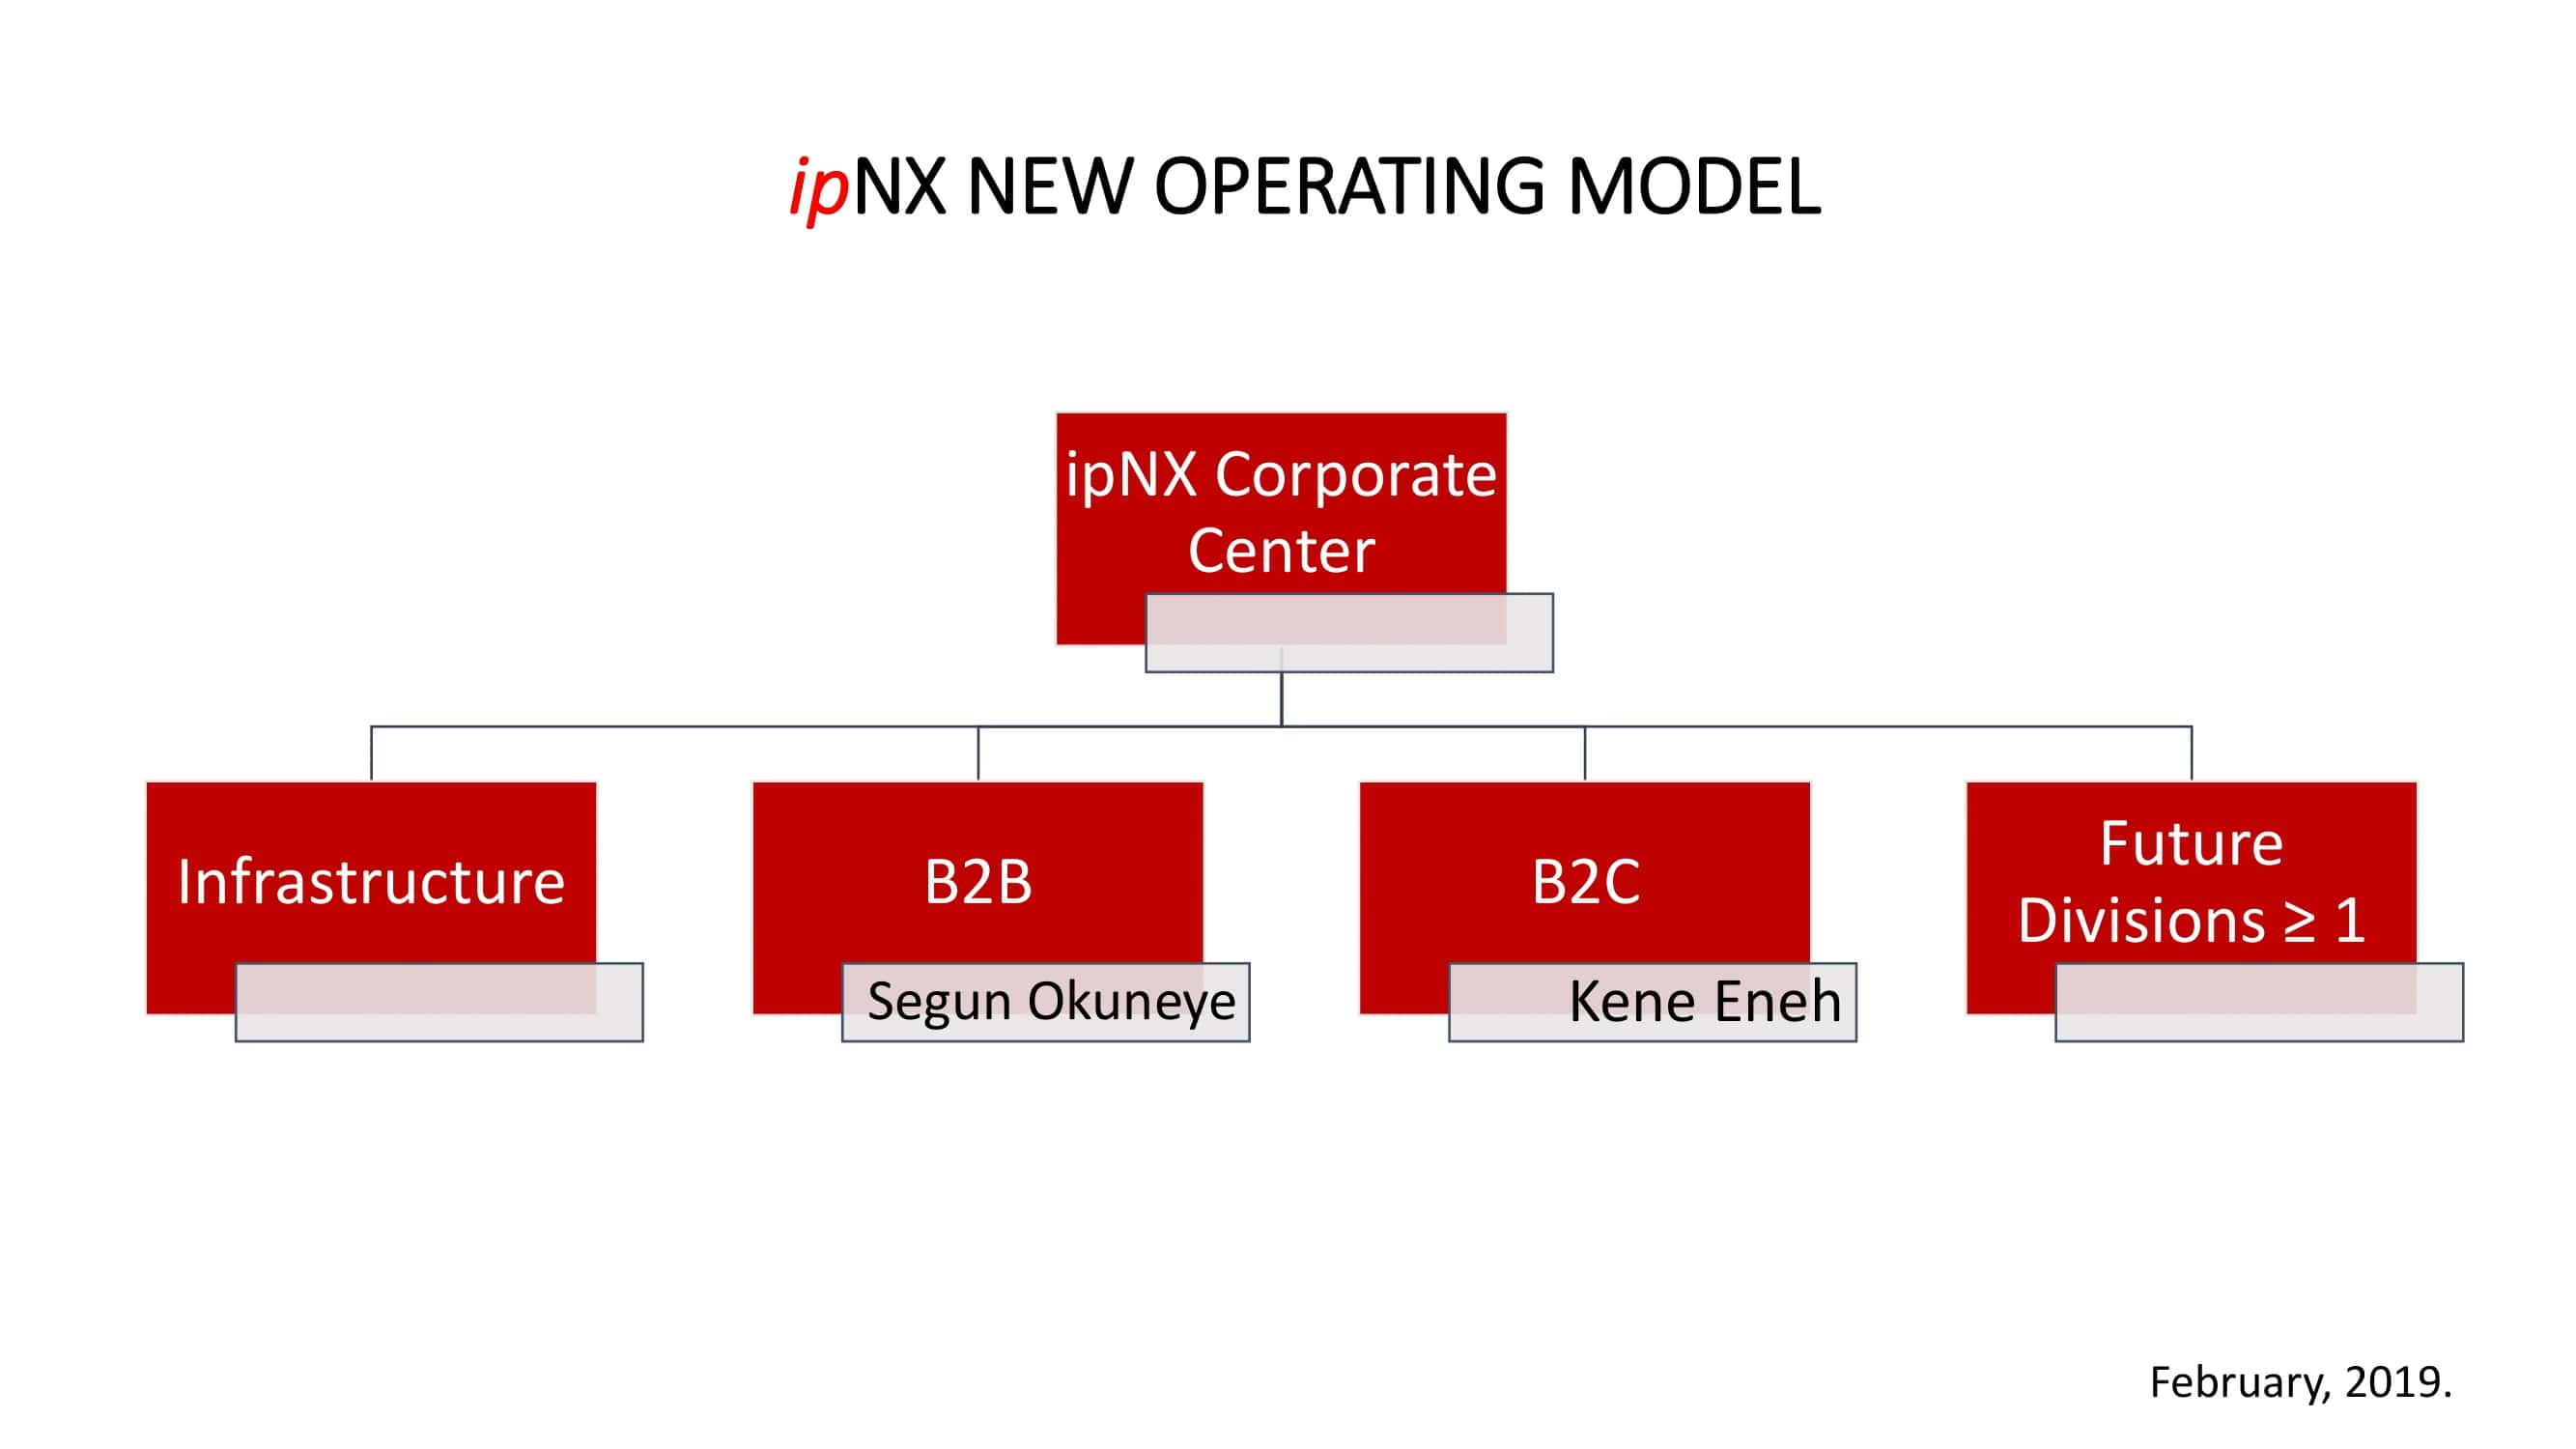
\includegraphics[width=1\textwidth]{./mainorg}
	\caption{\textit{ip}NX Main Organogram}
\end{figure}

\begin{figure}[h!]
	\centering
	\begin{subfigure}[b]{0.45\textwidth}
		\centering
		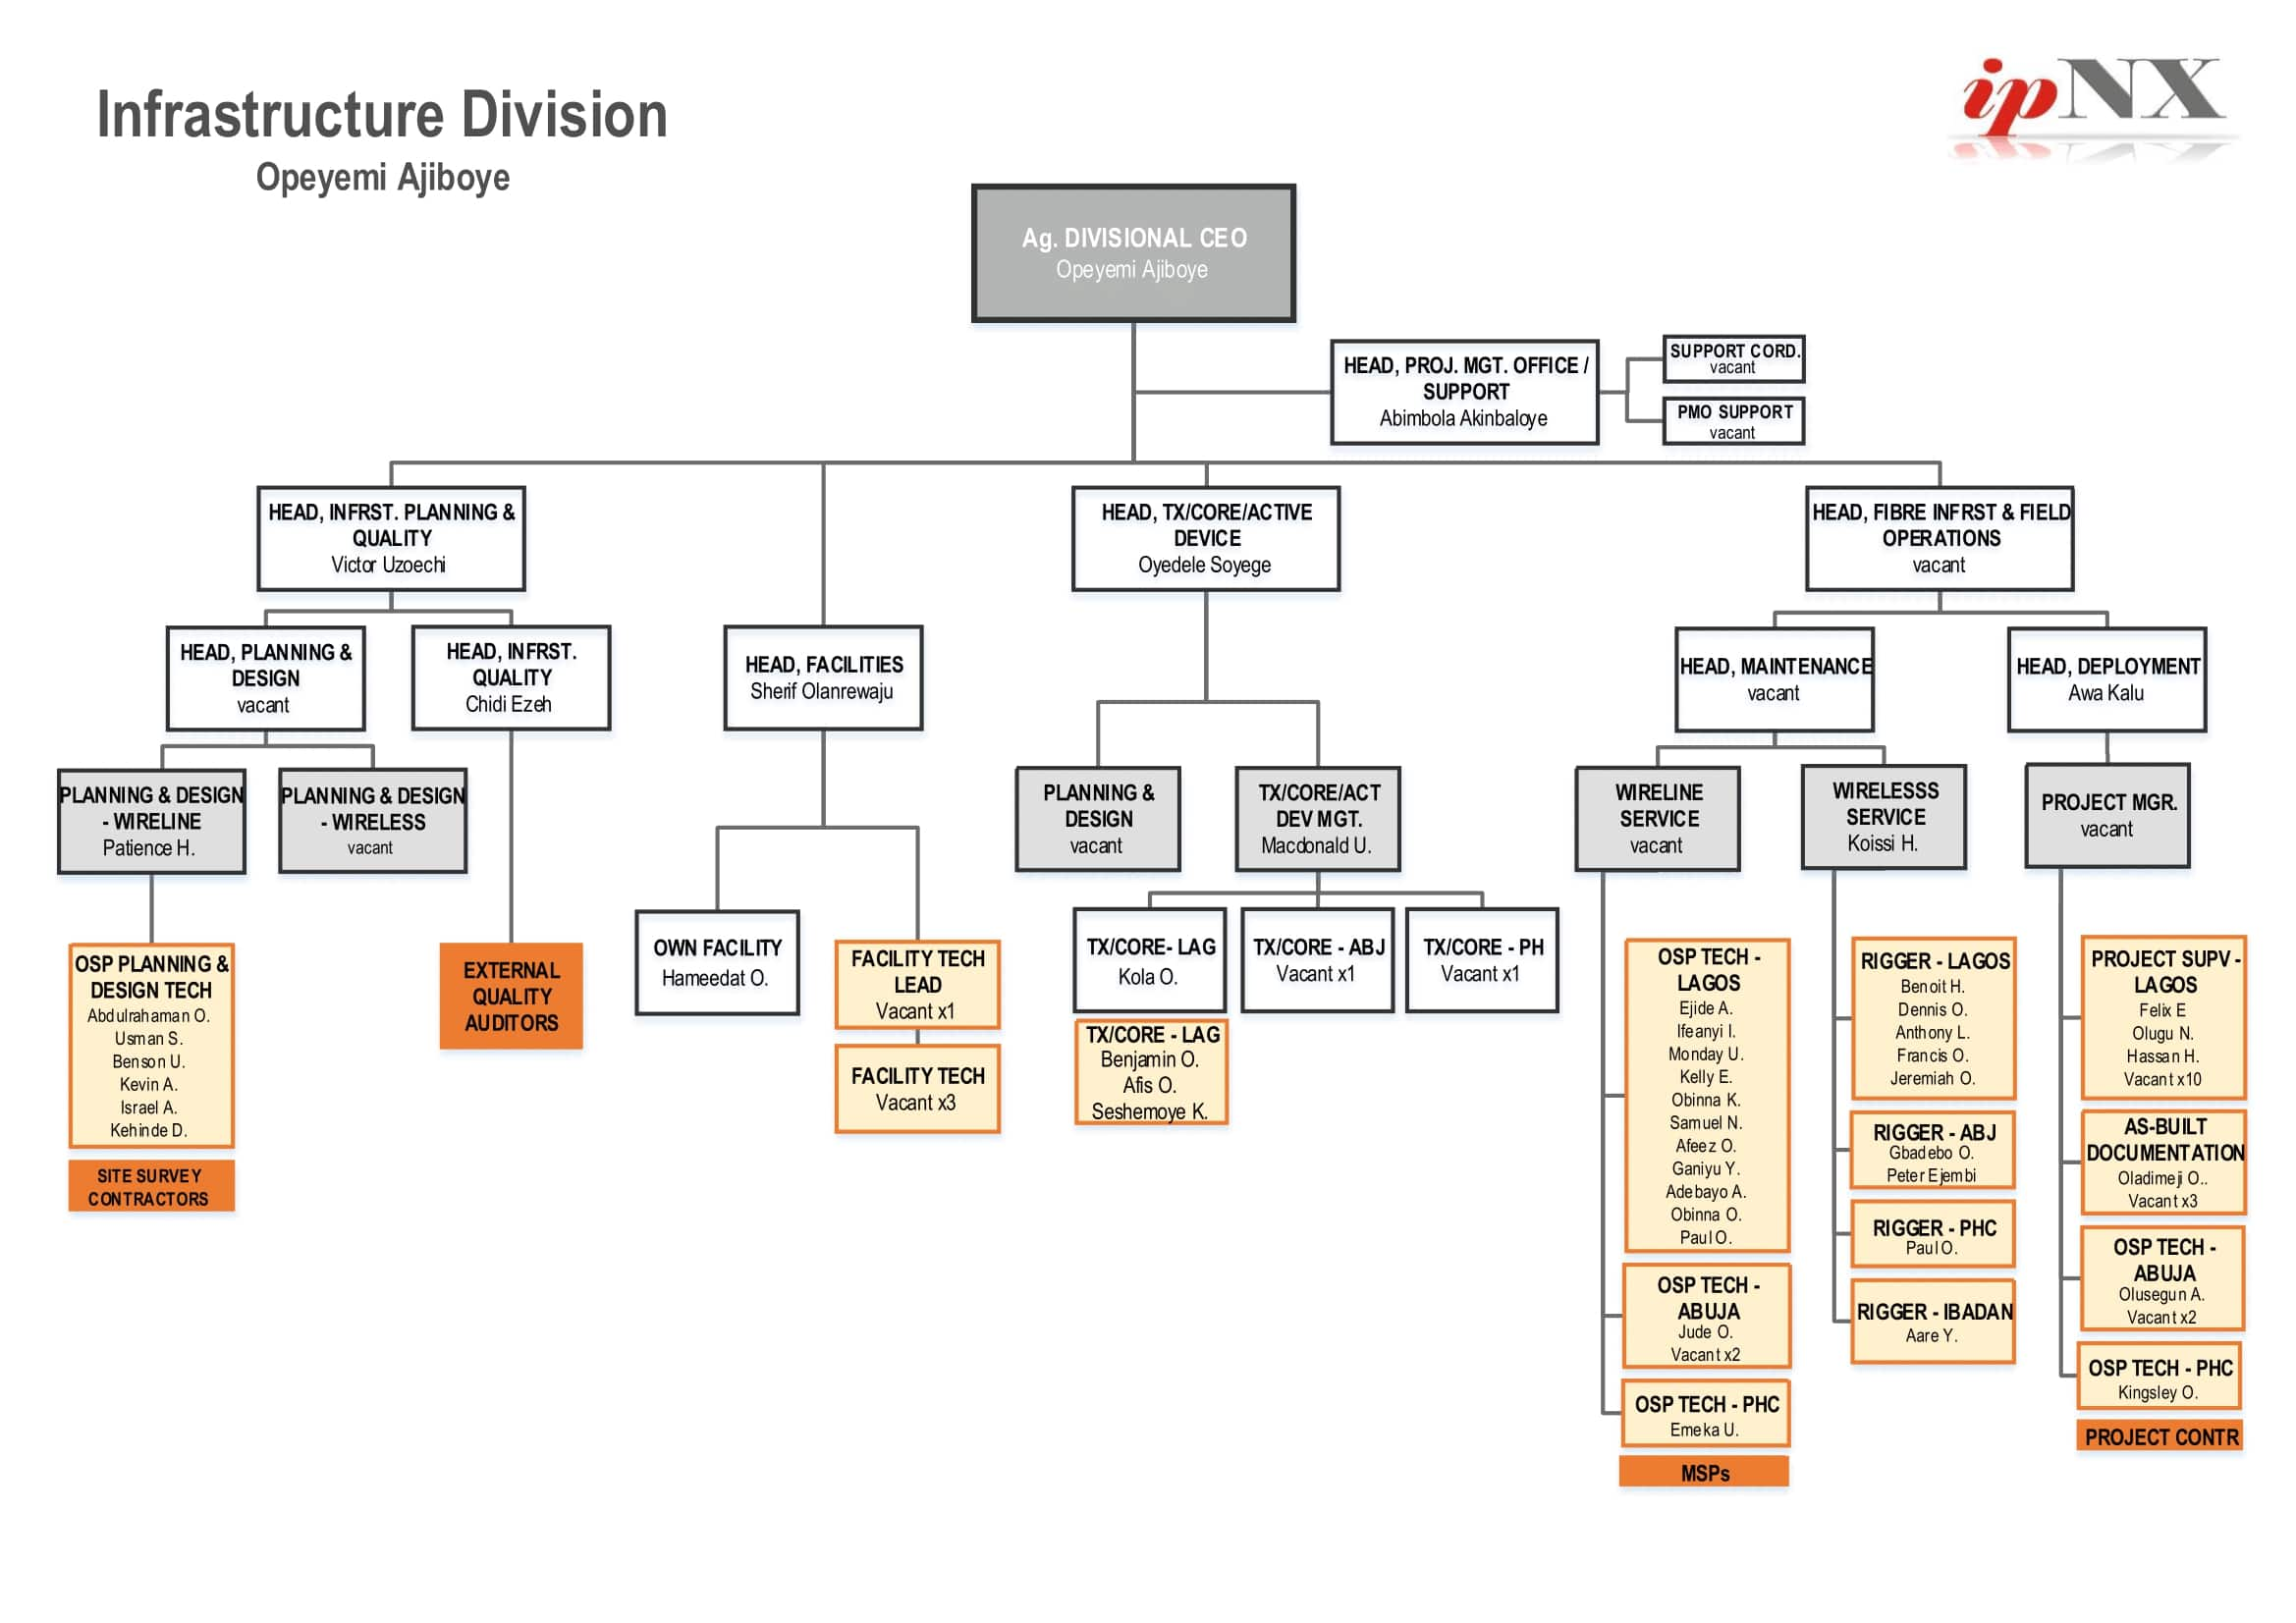
\includegraphics[width=\textwidth]{./InfrastructureOrgan}
		\caption{Infrastructure Organogram}
	\end{subfigure}
	\hfill
	\begin{subfigure}[b]{0.45\textwidth}
		\centering
		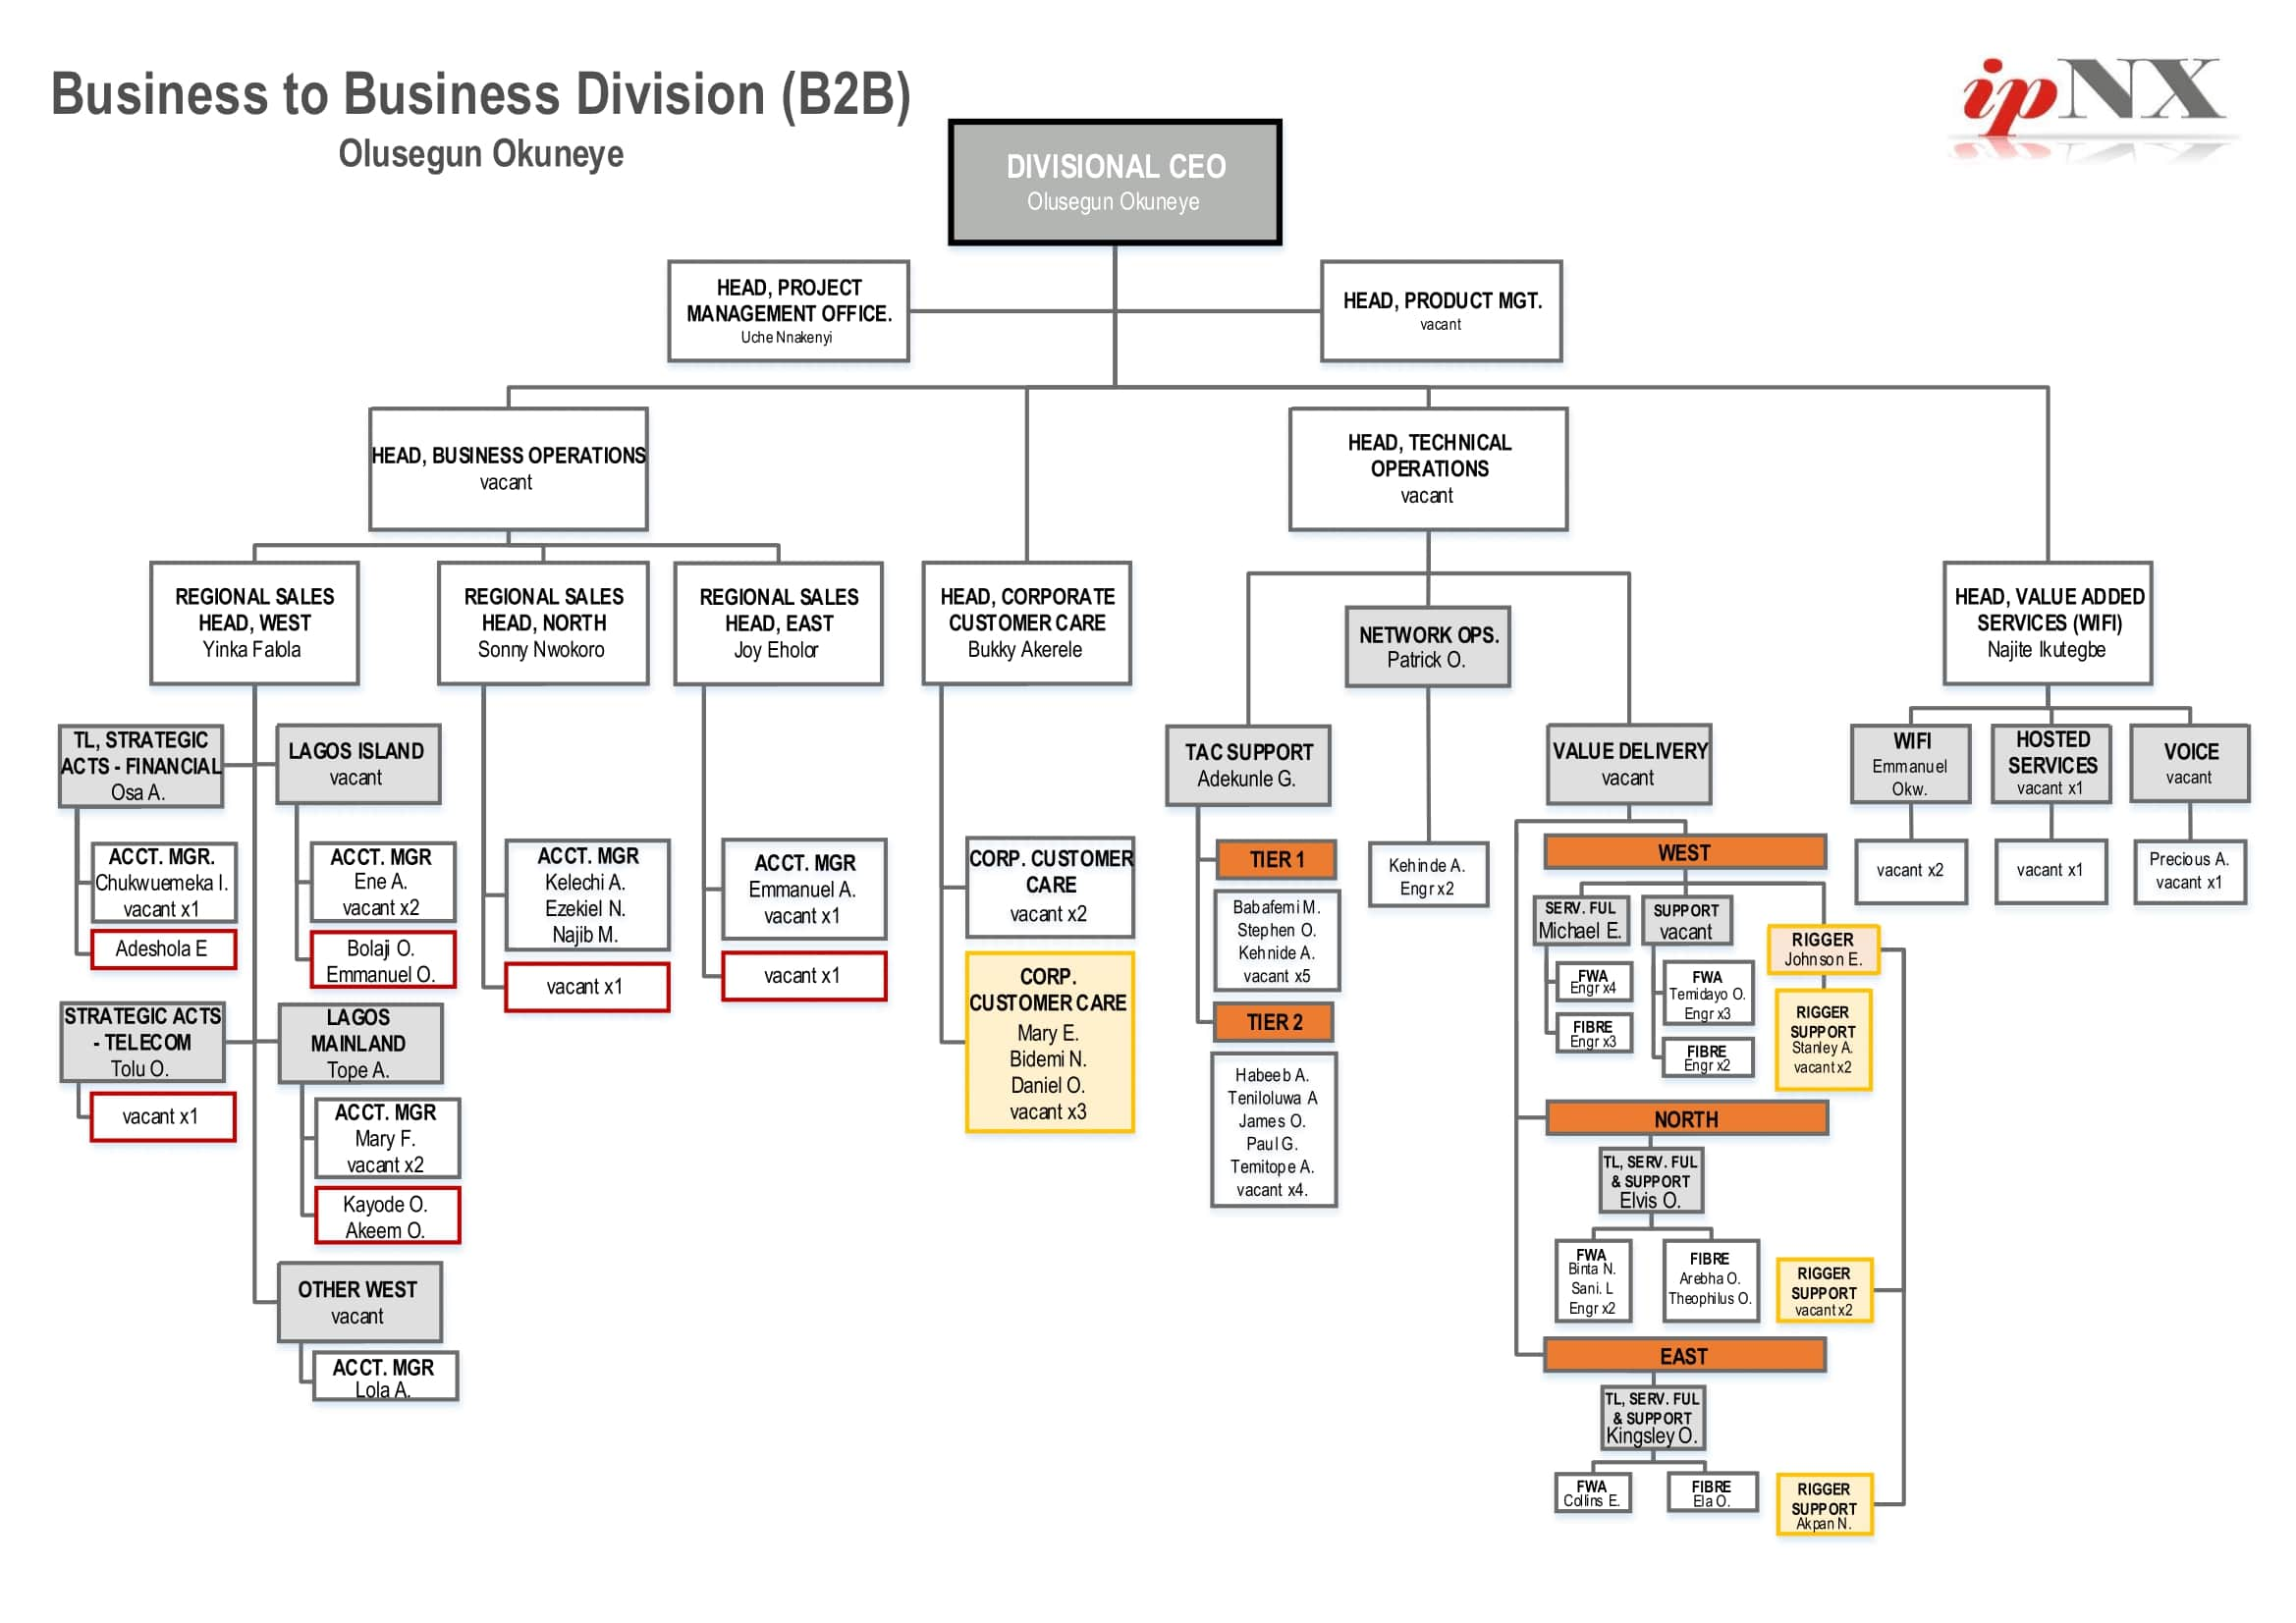
\includegraphics[width=\textwidth]{./B2Borg}
		\caption{Business Division(B2B) Organogram}
	\end{subfigure}
	\hfill
	\begin{subfigure}[b]{0.5\textwidth}
		\centering
		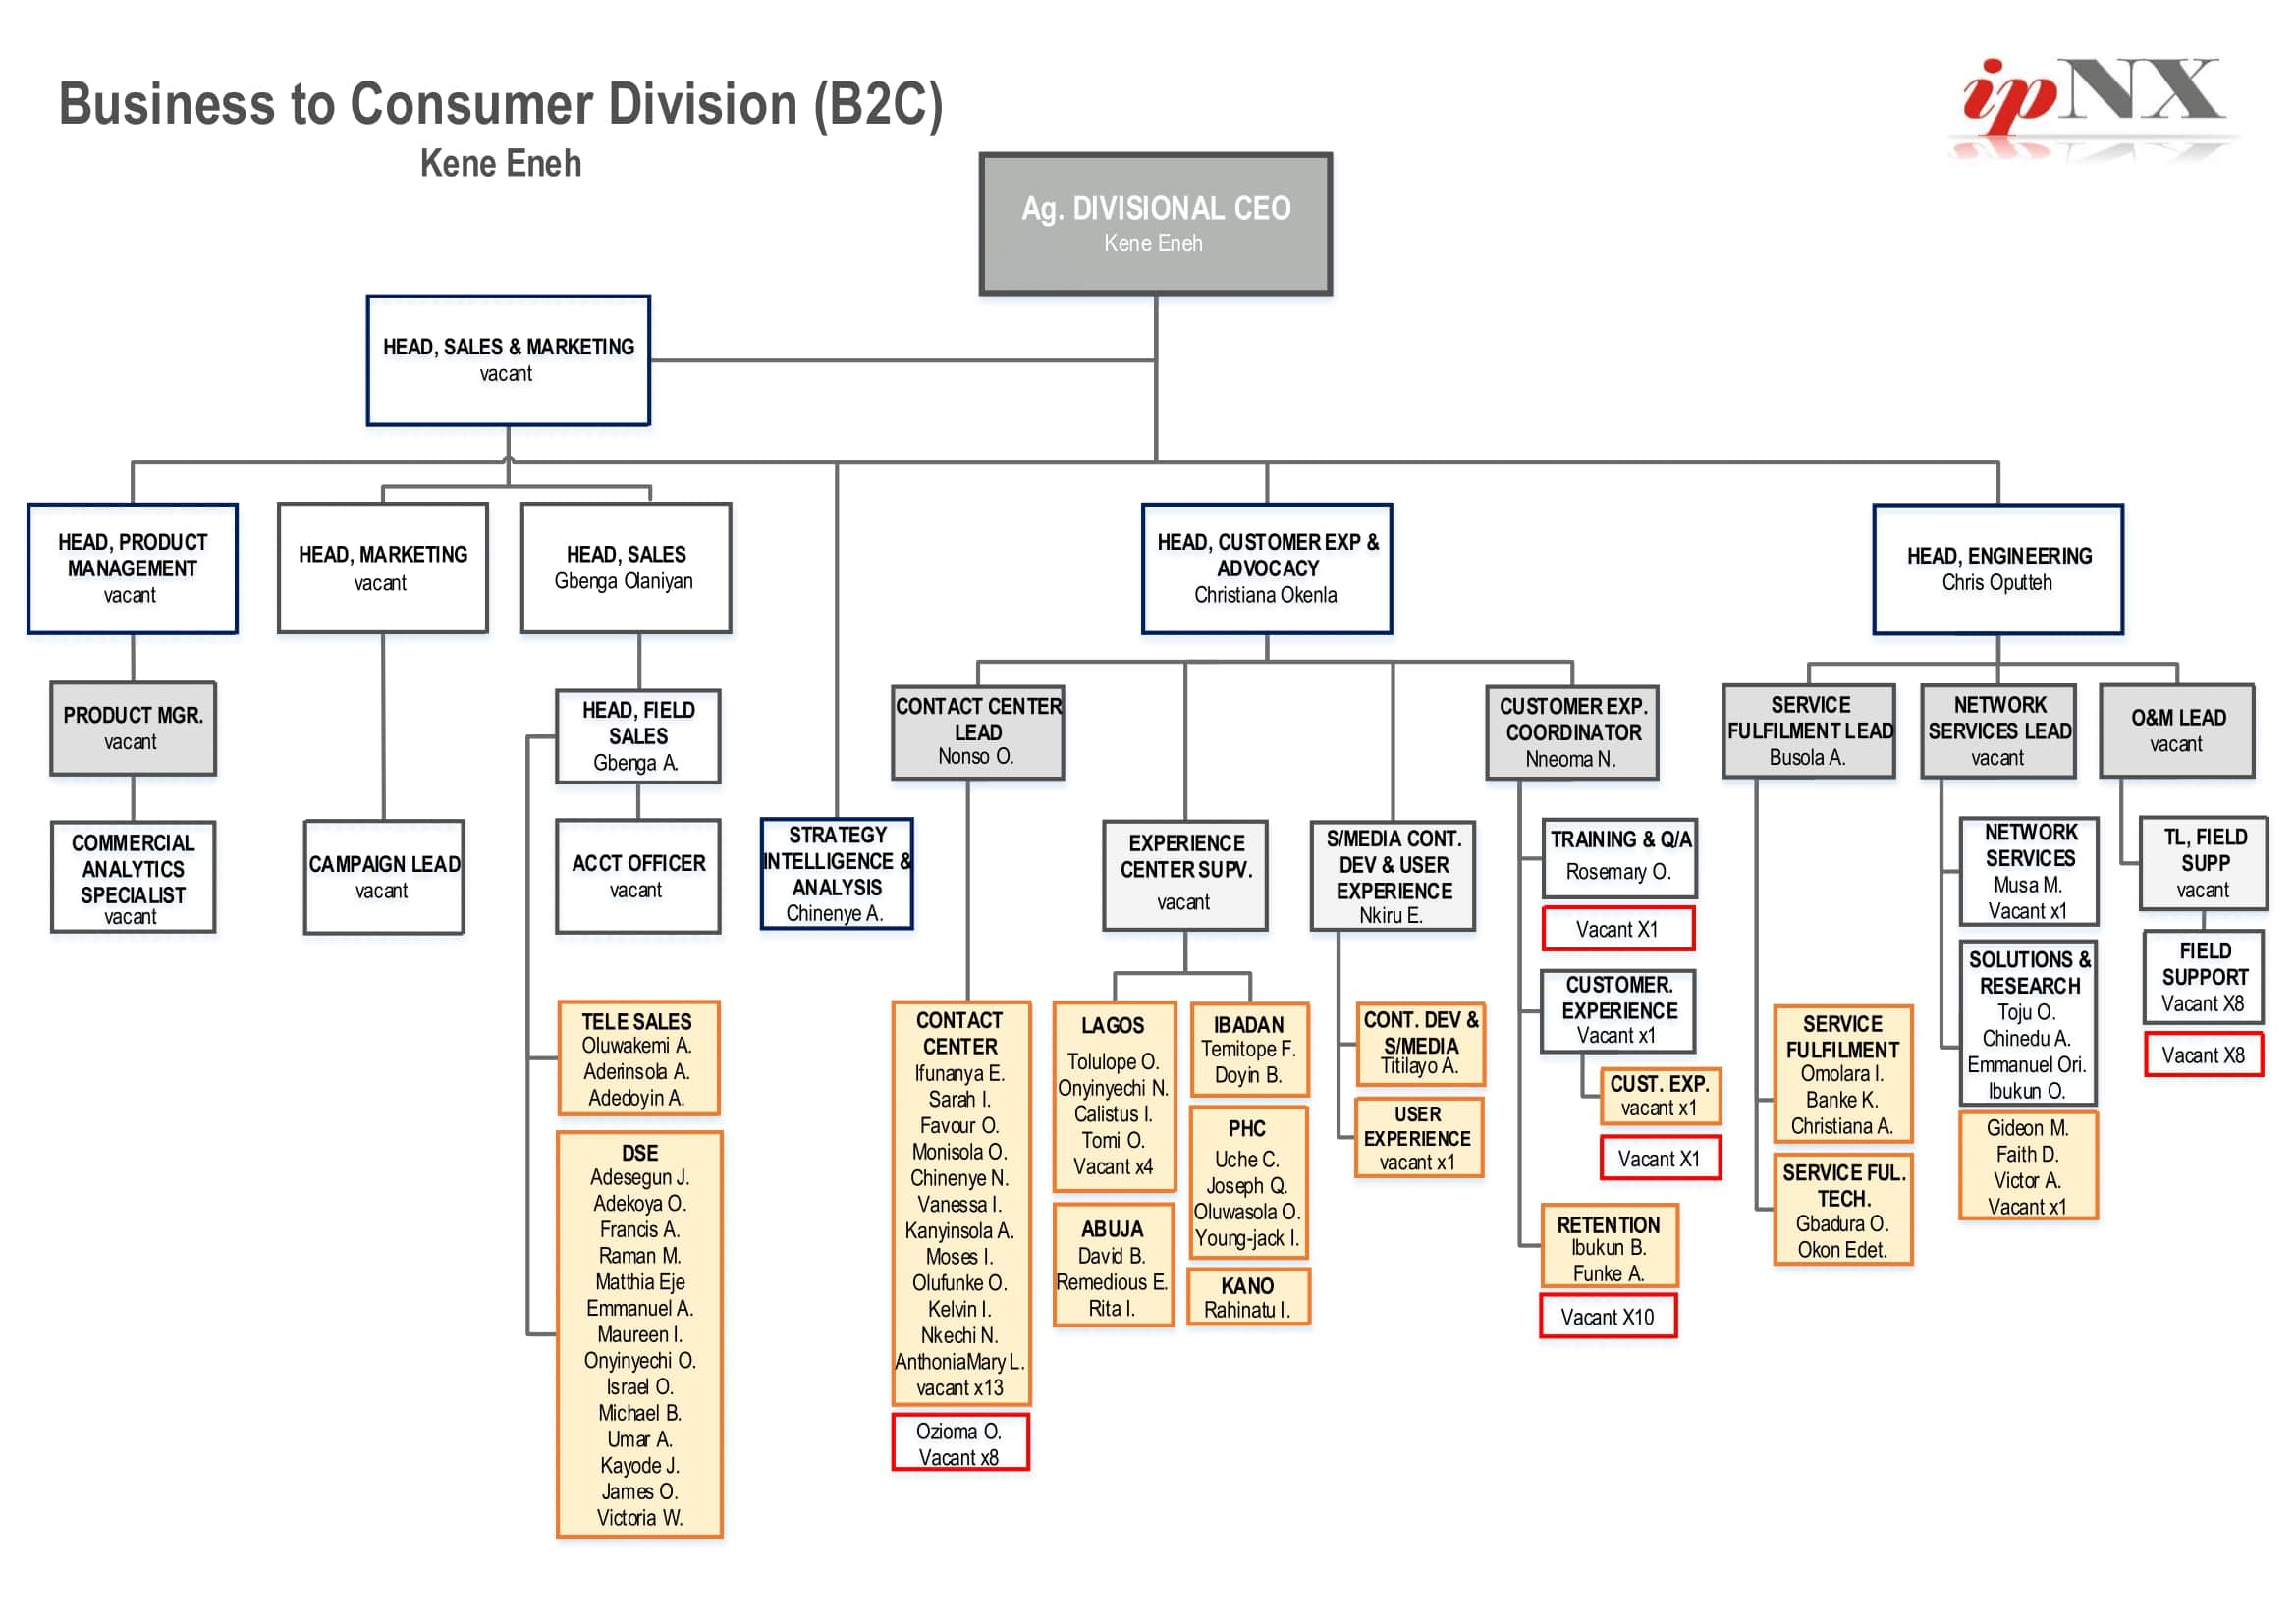
\includegraphics[width=\textwidth]{./B2COrgan}
		\caption{Retail Division(B2C) Organogram}
	\end{subfigure}
	\caption{Each division's organogram}
\end{figure}
\section{\textit{ip}NX Departments And Divisions}
\textit{ip}NX provides a range of network connectivity, and delivery of internet, telephony, television as well as cloud-based software application services for our clients. These services are delivered by teams working across multiple divisions and departments.
\subsection{\textit{ip}NX Departments}
\subsubsection{Human Capital Management}
Our Human Resource team brings out the best potential in every staff because here \textit{ip}NX, our people matter. Their talent, commitment, energy – plus the million and one things they bring to our business- makes us who we are. The way you think matters to us. we value creative thinking. So far, it has helped us recreate rules and we want more of it. If you like adventure, if you don't give up, if you are focus on getting results, we want you at \textit{ip}NX.
\subsubsection{Finance}
We would be nowhere without the expertise and insight of our finance teams. Our various teams include: Financial Accounting Revenue Assurance Treasury Billing The teams are there to understand, support and challenge the business, making sure we are doing everything we can to run efficiently by providing the financial expertise required to grow our business to profitable levels and heights. If you have an eye for numbers and a brain for planning, what are you waiting for?
\subsubsection{Legal, Risk And Compliance}
Our Legal area has a big impact on our actions. Fortunately, we can rely on the counsel, creative thinking and sound judgment of the Law, Risk and Compliance team to unravel the finer points and keep us on the right track. If you know you are a champion of business integrity; are good at building constructive business relationships with our customers, partners, local communities, or the government; strive to protect and promote innovation, enterprise, then join us for a career with our LRC team.
\subsubsection{Customer Experience \& Advocacy}
When our customers need support and advice, or they want to get something sorted out, they deserve the right help, right on time. Everyone in customer service loves to make a difference because they strive for excellence. They won’t stop until they can see the smile of satisfaction on the customer’s face. Very simply put, we obsess over our customer. On joining the Customer service team, you will be the voice of \textit{ip}NX. And whatever the next call brings, your goal remains the same; to delight and dazzle with your knowledge and commitment. If you can throw in some pleasant surprises along the way, everyone is a winner.
\subsubsection{Health, Safety And Environment}
\textit{ip}NX Health, Safety and Environmental team is responsible for development, oversight, and management of environmental health and safety programs that protect the \textit{ip}NX working environment, provide safe and healthy conditions for work and comply with applicable laws and regulations. It is the team's goal is to pro vide responsive service and critical support to ensure that \textit{ip}NX is a safe and healthy environment in which to work, study, and live. If you are an expert in what you do and love safety, apply to join our HSE team.
\subsubsection{Marketing}
\textit{ip}NX Marketing Department plays a massive role in promoting the mission and business of \textit{ip}NX. \textit{ip}NX Marketing team's main focus is to understand our customers, their values, and perception and make sure they get it – through our amazing services because \textit{ip}NX was born to disrupt – but with a purpose.  If you can wow our customers with \textit{ip}NX brand, you might just fit right in with this team.
\subsubsection{Internal Audit}
Our Internal Audit team provides \textit{ip}NX with unbiased, objective and constructive views that help companies succeed. Our internal audit team examines and evaluates the policies, procedures and systems which are in place to ensure the reliability and integrity of information, compliance with policies, plans, laws and regulations; the safeguarding of the assets; and the efficient use of resources. We are looking for professionals who take pride in their work.
\subsubsection{Corporate Services}
Our Corporate services are made up of Human Capital Management, Administrative Services, Facility Management, etc. They provide services to our people. They make sure we get the best employees who remain the best employees on top of their game; they make sure we have both the physically and mentally enabling environment to support and push out our creativity. At \textit{ip}NX, we want to work with people who know the next best idea is just around the corner – and who have the ambition, creativity, and passion for going after it.
\subsubsection{Supply Chain Management}
Our SCM team helps cordinate and integrate  seamless information, material and finance flow from suppliers to customers, so that we have an excellent customer service, an ideal inventory management and low unit cost. At \textit{ip}NX, our SCM team has the prime responsibility of integrated planning, sourcing and deployment of material connected to our network services . If you know you have the expertise for this job, why not join our SCM team.
\subsubsection{Information Systems And Technology}
As an organization that is in love with leading edge innovation and services, it is no wonder that our IS\&T team plays a crucial role. The team provides exceptional technological services and support. Our team enables efficiency, productivity and simplicity both internally and externally, helping us to grow. Joining our IS\&T team means you will help keep our internal IT running smoothly by creating and maintaining our systems and applications.
\subsubsection{Fibre Project And Rollout}
Our Fibre Project and Rollout team are our hunchos when it comes to rolling out our network fibres direct to business areas and homes. If you have a passion for  success and want to make a difference for customers every day, join our Fibre Project and Rollout Team.
\subsubsection{Admin Services}
Every organization needs somebody to coordinate it. That job is for the \textit{ip}NX administrative team. The administrative team brings its conscientious planning, attention to detail and flexible thinking to the heap of projects. They help make sure things run like a well-oiled clock. This means organizing everything from staying on top of day to day administration, prioritizing and managing real estate and other assets, getting involved in team strategy and company – wide objectives. If you want to join our administration team, there is always plenty of opportunity to make your mark.
\subsubsection{Research And System Architecture}
The \textit{ip}NX Research and System Architecture team is reinventing the technology world every day. The Research and System Architecture team is in charge of all our research and development and are also responsible for coming up with tomorrow services that meet the needs for our today’s customers. They look for ways to do it cheaper, faster, and better. We are looking for those who have the drive and passion for technology.
\subsection{\textit{ip}NX Divisions}
\subsubsection{Infrastructure Division}
\textit{ip}NX network is always on duty, always in demand. That means it has to be reliable. This all comes down to the diligence and support of our network services team.  Whether fixed-voice and data; mobility; and IT services, they make sure our network is ever available. This means our customers’ experience is in their hands. They are there to trouble shoot malfunctions and make the network service bigger, better, faster and stronger. If you are someone who can resolve issues, develop ideas to enhance a growing network and most importantly, work with the \textit{ip}NX team and embrace the values we uphold, then you have what it takes to be part of \textit{ip}NX community.
\subsubsection{Retail Division}
\subsubsection{Business Division}
\chapter{Projects Done and Experiences Gained}
\section{Preliminaries}
This section gives a brief introduction to or exposes the technologies used while implementing the projects assigned to me.
\subsection{Software development process overview at \textit{ip}NX}
In IEEE standard Glossary of Software Engineering
Terminology, the \ac{SDLC} is: “The period of time
that starts when a software product is conceived and ends
when the product is no longer available for use”. This circle typically includes the following stages:
\begin{enumerate}
	\item Planning and requirement analysis: Each \ac{SDLC} model starts with Planning and requirement analysis, in which stakeholders of the process plan and discuss the requirements for the final product with the goal of a detailed definition of the system requirements.
	\item Designing project architecture: In this stage, the developers engage in designing the architecture of the software product and any surfaced technical questions are discussed by all the stakeholders, including the customer. Technologies which will be used, team load, limitations, duration and budget are also defined.
	\item Development and programming: Having approved the requirements stated, the process comes to this stage – actual development. Programmers incept writing of source codes to align with the defined requirements, System administrators adjust the software environment, front-end programmers develop the user interface of the program and the logics for its interaction with the server. 
	The programming by itself assumes four stages:
	\begin{itemize}
		\item Development of Algorithms
		\item Writing of Source Codes
		\item Source codes compilation
		\item Unit testing and debugging
	\end{itemize}
	\item Testing: This is the phase where comprehensive testing and debugging of the developed software product take place. All the code flaws missed during the development are detected, documented, and passed back to the developers to fix. The testing process repeats until all the critical issues are removed and software workflow is stable.
	\item Deployment: When the program is finalised and has no critical issues, it is time to launch it for the end users and this happens in this stage.
	\item Maintenance
\end{enumerate}

According to \citet{Sharma:2015}, General software process models are:
\begin{enumerate}
	\item  Waterfall model
	\item  Prototype model
	\item  Rapid application development model (RAD)
	\item  Incremental model
	\item  Spiral model
	\item  Agile
	\item  V-shaped model
\end{enumerate}

These models are depicted in Figure 3.1 below:
\begin{figure}[htbp]
	\centering
	\begin{subfigure}[b]{0.45\textwidth}
		\centering
		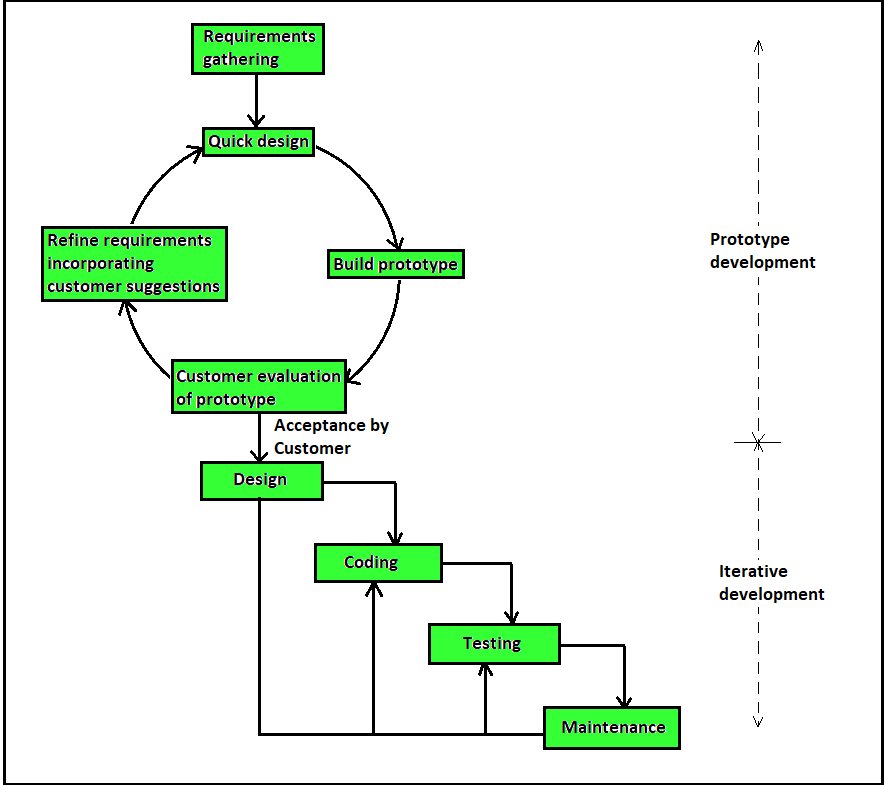
\includegraphics[width=\linewidth]{./Prototyping-model}
		\caption{Prototype Model, Source: \citet{Kumar:2020}}
		\label{fig: 1}
	\end{subfigure}
	\hfill
	\begin{subfigure}[b]{0.45\textwidth}
		\centering
		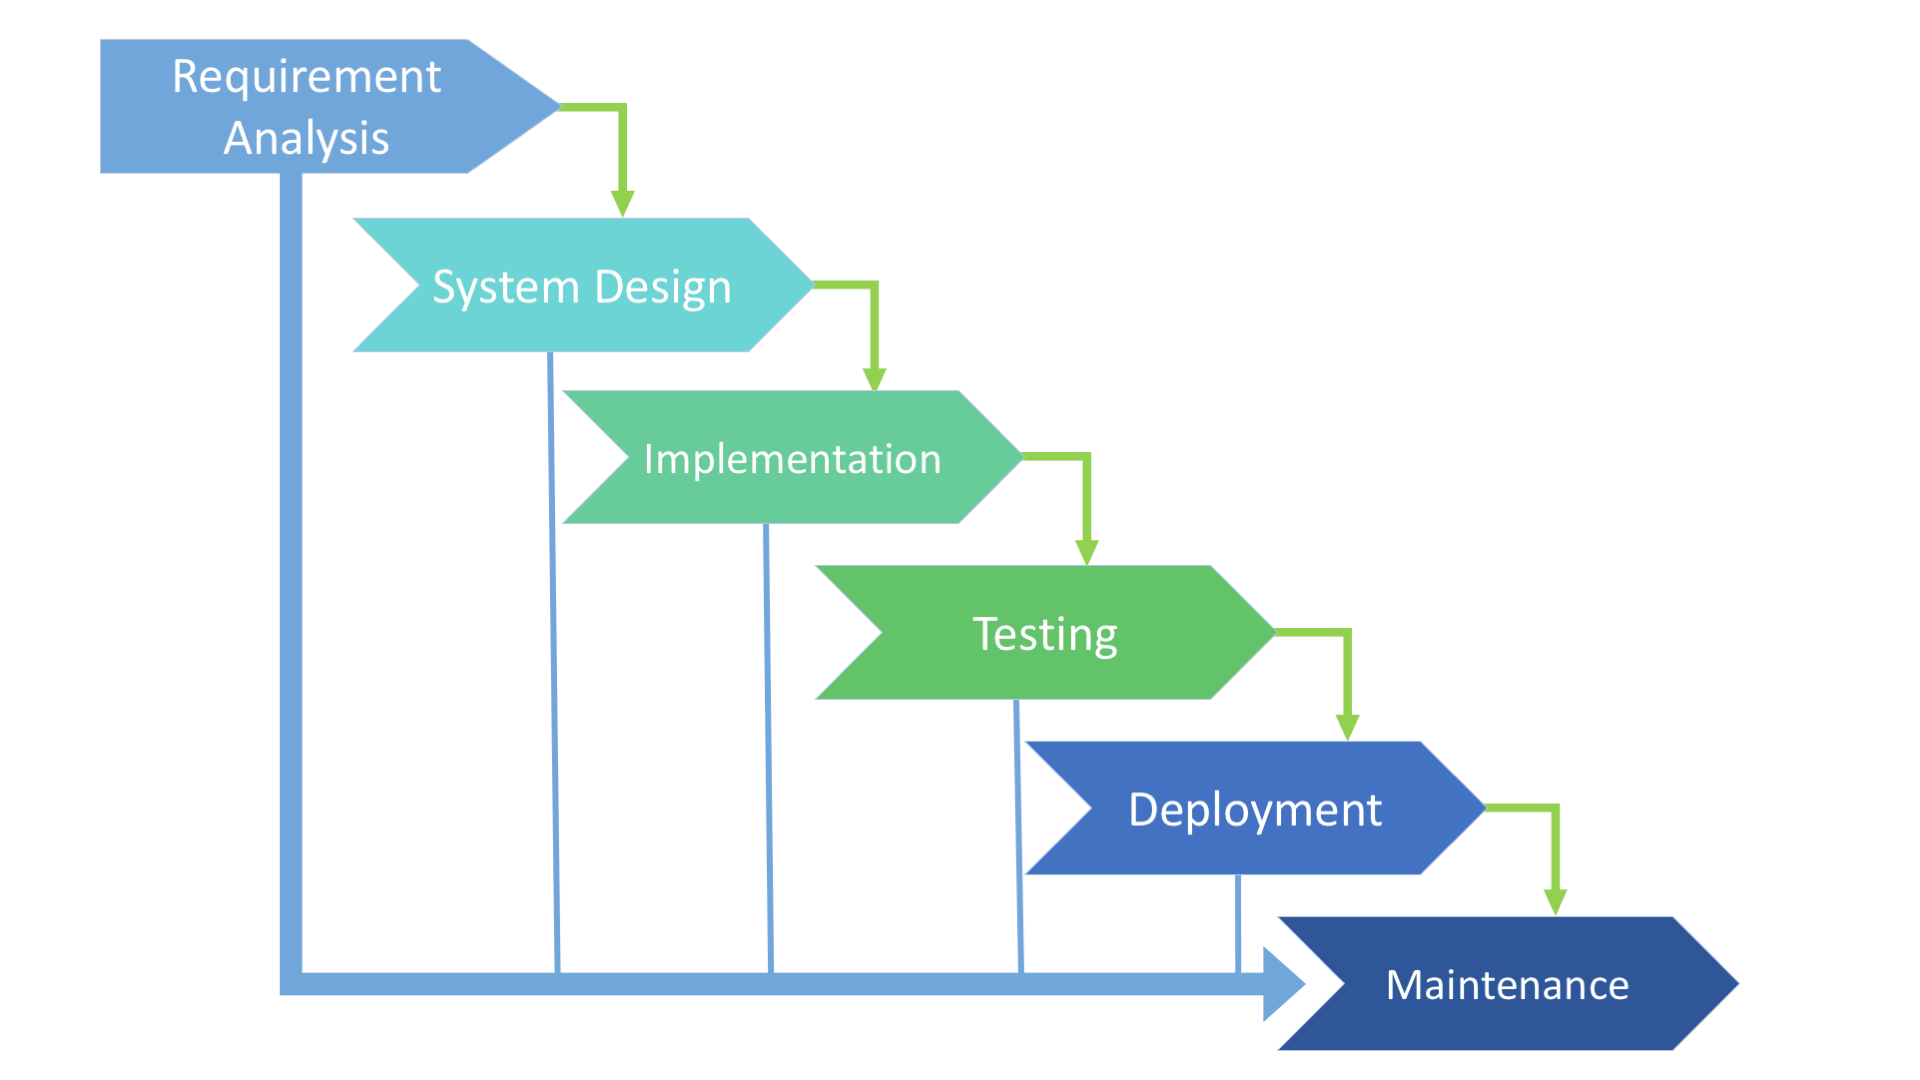
\includegraphics[width=\linewidth]{./waterfall}
		\caption{Waterfall model, Source: \citet{Team:2017}}
		\label{fig: 2}
	\end{subfigure}
	\medskip
	\begin{subfigure}[b]{0.45\textwidth}
		\centering
		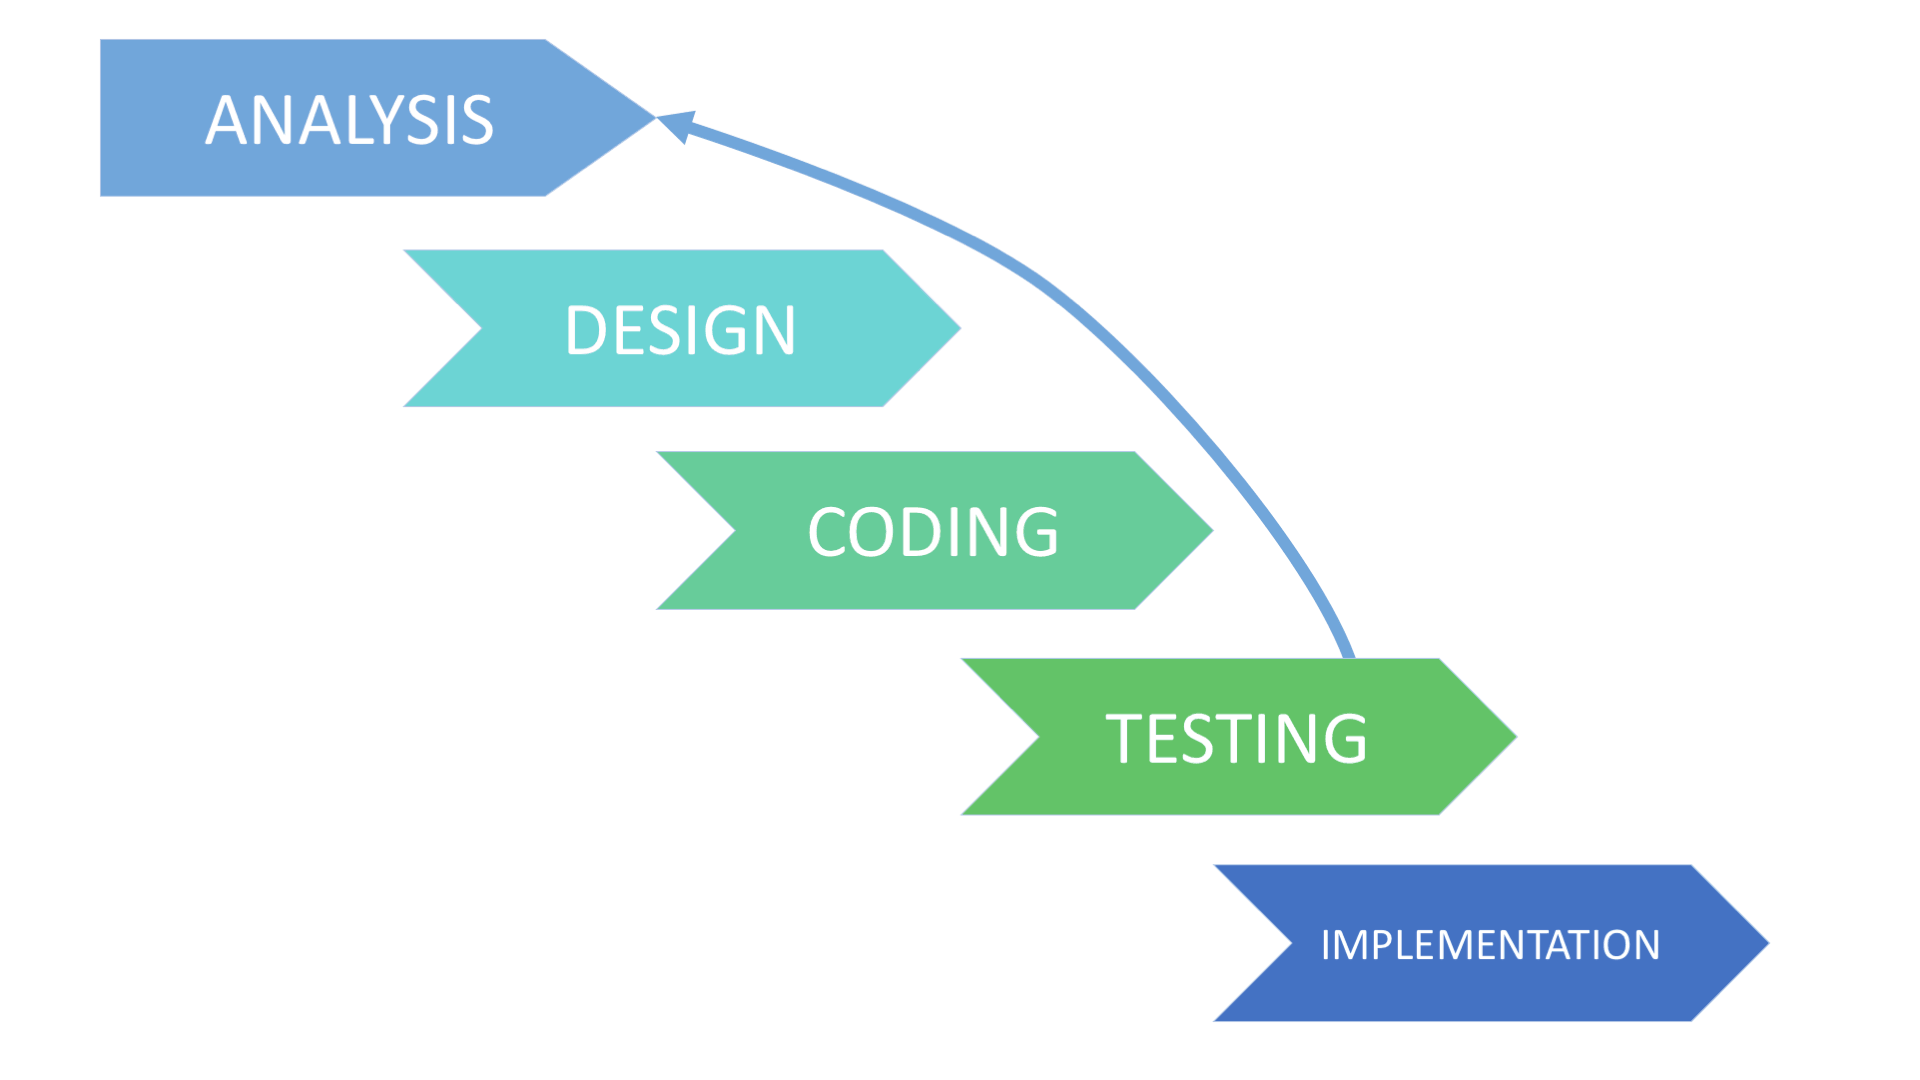
\includegraphics[width=\linewidth]{./iterative}
		\caption{Incremental model, Source: \citet{Team:2017}}
		\label{fig: 3}
	\end{subfigure}
	\hfill
	\begin{subfigure}[b]{0.45\textwidth}
		\centering
		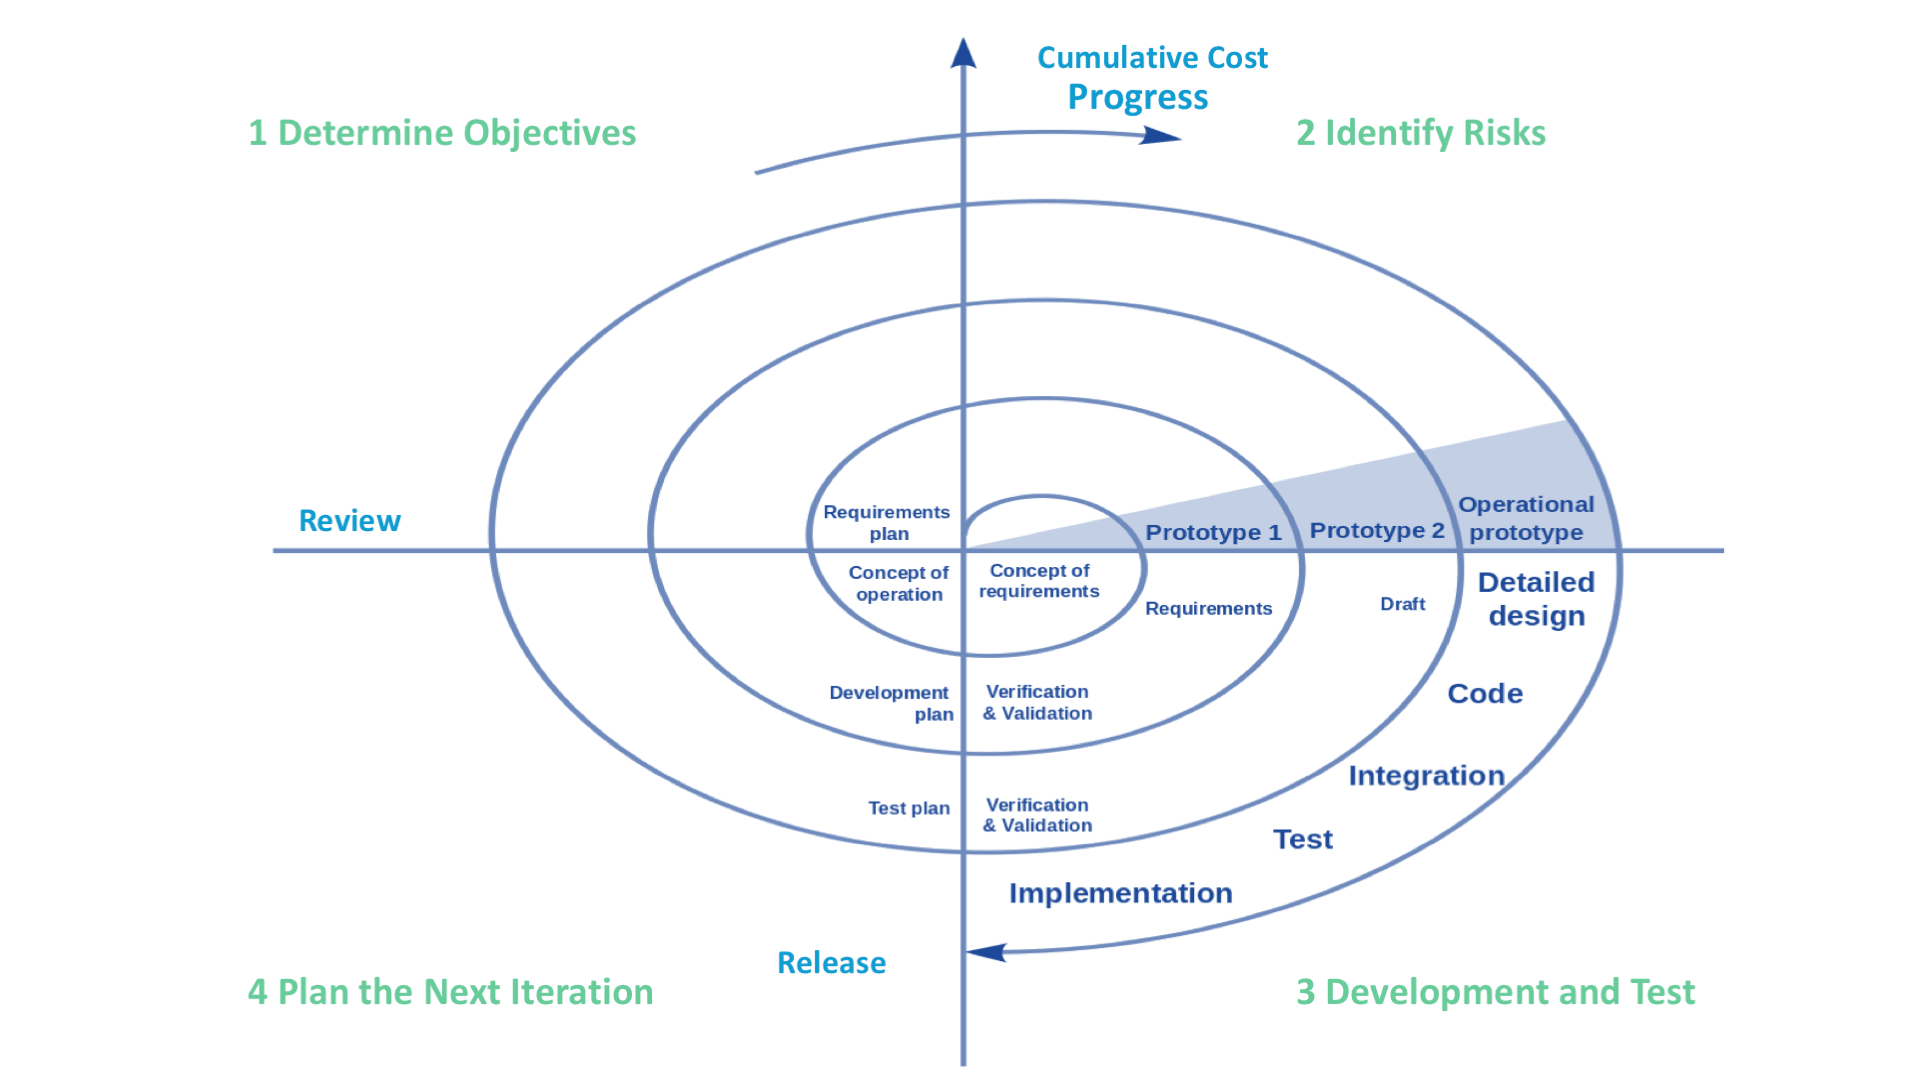
\includegraphics[width=\linewidth]{./Spiral}
		\caption{Spiral model, Source: \citet{Team:2017}}
		\label{fig: 4}
	\end{subfigure}
	\medskip
	\begin{subfigure}[b]{0.45\textwidth}
		\centering
		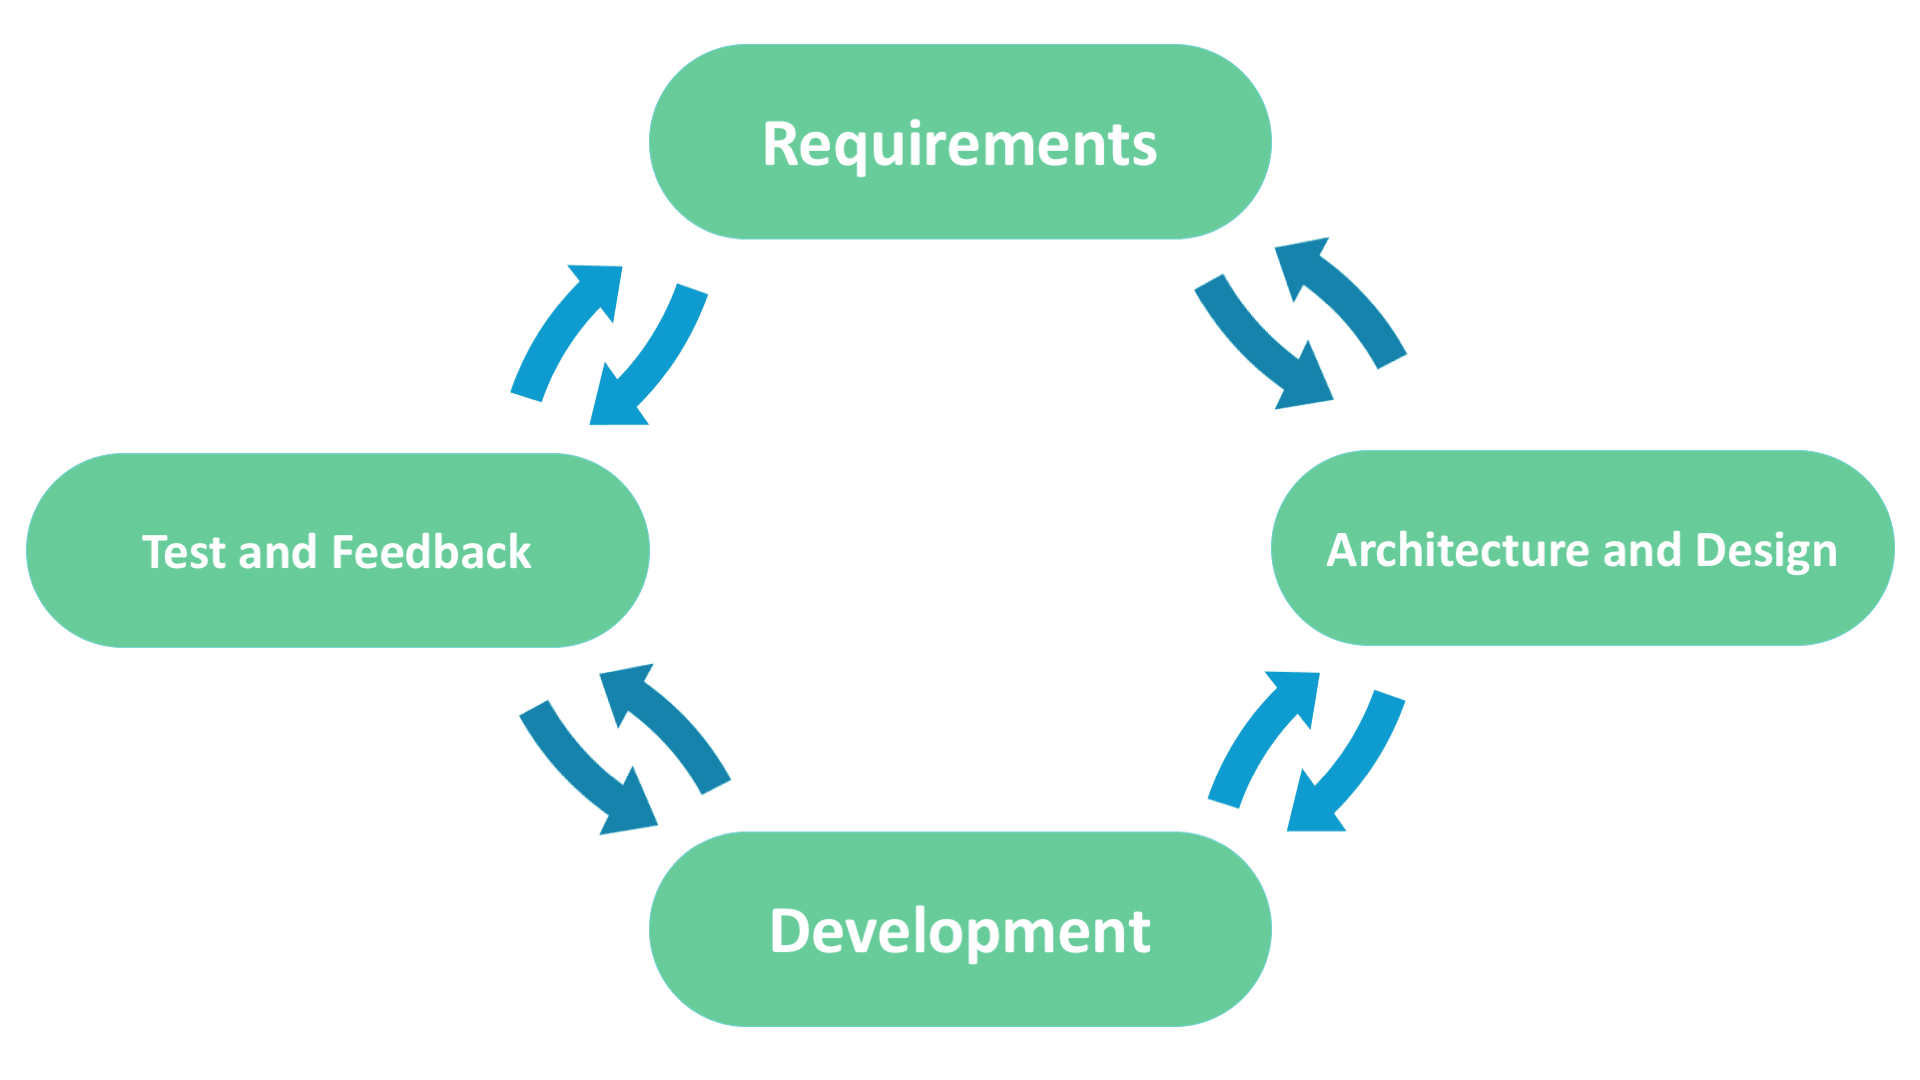
\includegraphics[width=\linewidth]{./Agile}
		\caption{Agile model, Source: \citet{Team:2017}}
		\label{fig: 5}
	\end{subfigure}
	\hfill
	\begin{subfigure}[b]{0.45\textwidth}
		\centering
		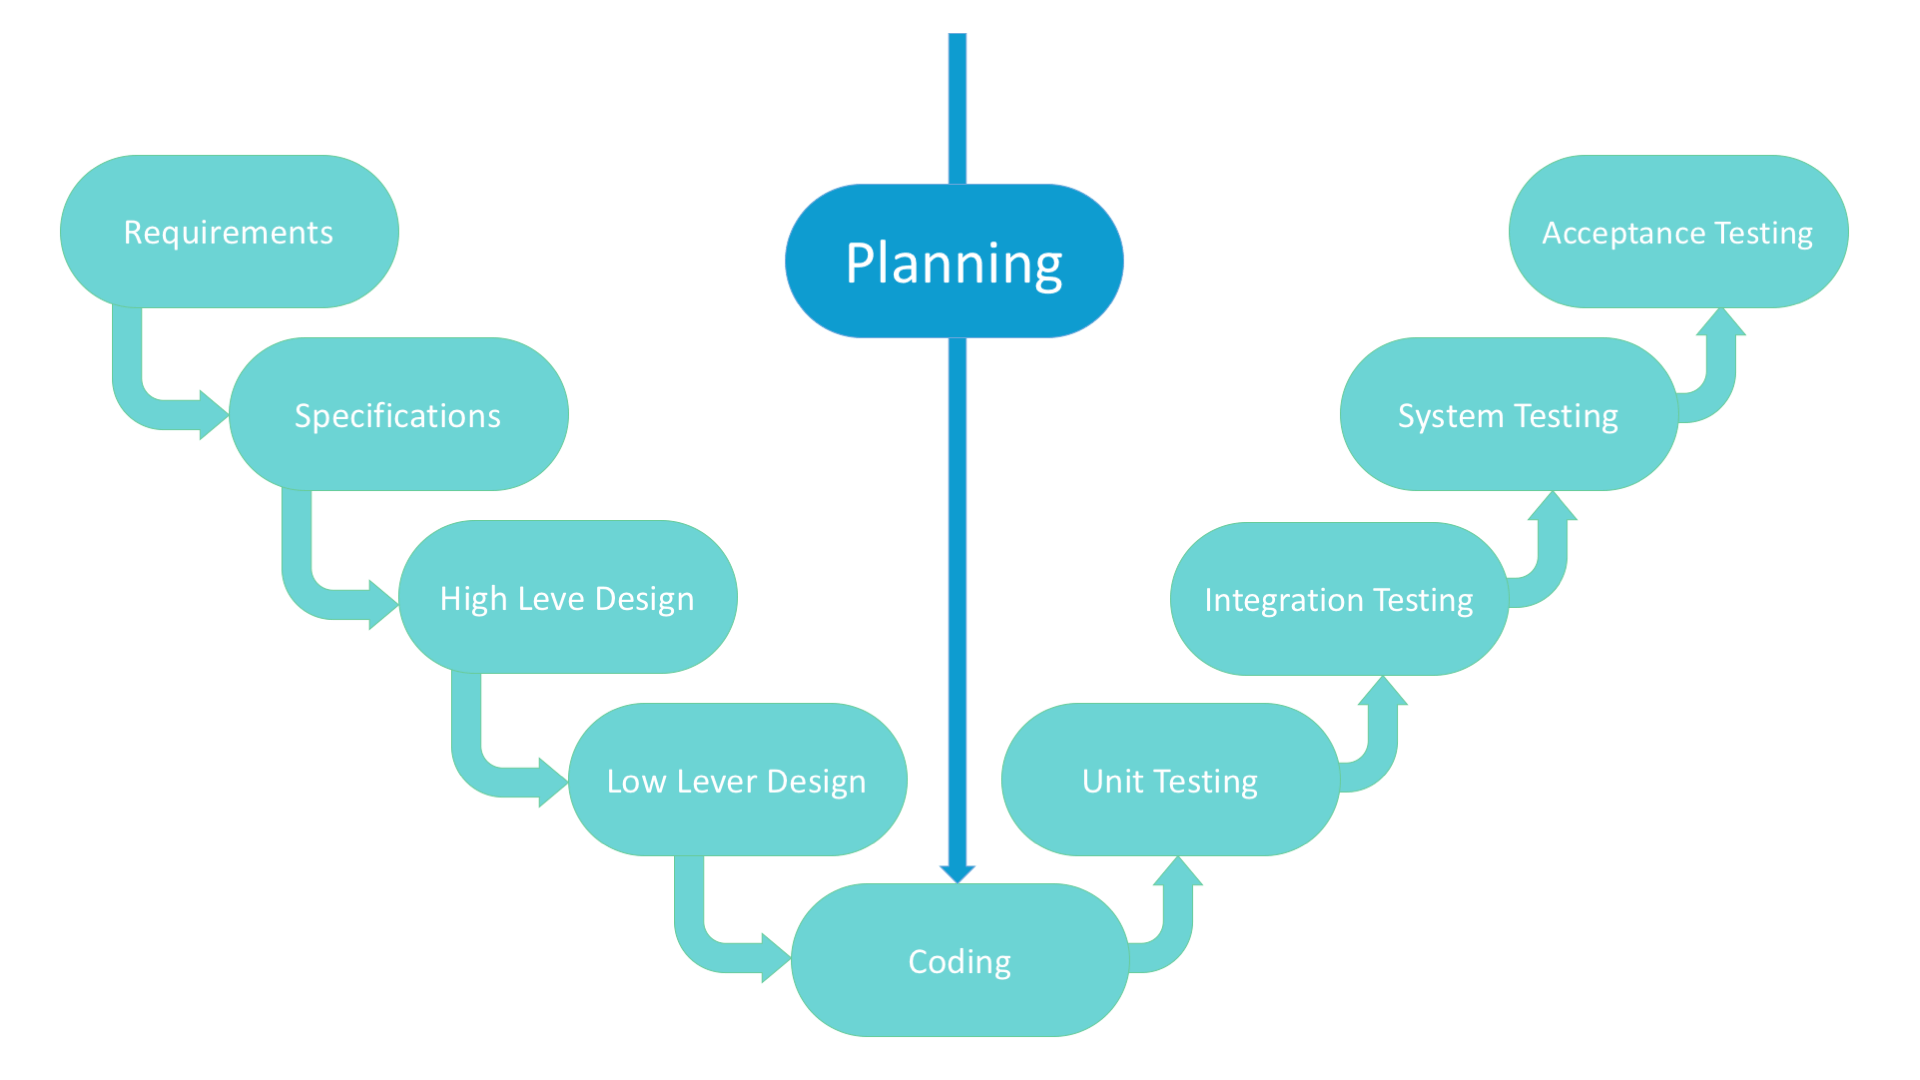
\includegraphics[width=\linewidth]{./V-Shaped}
		\caption{V-shaped model, Source: \citet{Team:2017}}
		\label{fig: 6}
	\end{subfigure}
	\medskip
	\begin{subfigure}[b]{0.5\textwidth}
		\centering
		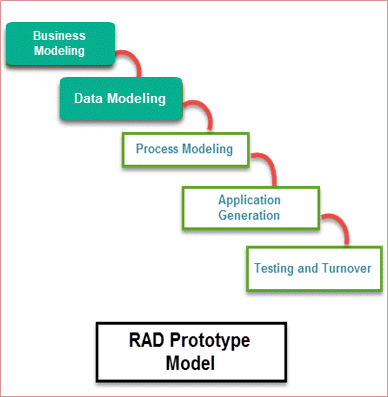
\includegraphics[width=\linewidth]{./rad}
		\caption{Rapid application development model (RAD)}
		\label{fig: 7}
	\end{subfigure}
\caption{\ac{SDLC} Models}
\end{figure}
\subsubsection{Comparison of \ac{SDLC} Models}
Table: 3.1 compares the General software process models on different Parameters as listed and compared in \citet{Sharma:2015}.
\begin{table}[htbp]
	\caption{ Comparison of various \ac{SDLC} Models on different Parameters}
	\label{Table: 3.1}
	\resizebox{\columnwidth}{!}{\begin{tabular}{l l l l l l l l}
		\toprule
		\textbf{Model/Features} & \textbf{Waterfall} & \textbf{Prototype}& \textbf{RAD} & \textbf{Incremental} & \textbf{Spiral} & \textbf{Build \& Fix} & \textbf{V-shaped}\\
		\midrule
		Well defined requirements & Yes & No & Yes & No & No & No & Yes\\
		User involvement in all phases & Only at beginning & High & Only at beginning & Yes(Intermediate) & High & No & No\\
		Risk analysis & Only at beginning & No Risk analysis & Low & No Risk analysis & Yes & No & Only at beginning\\
		Overlapping phases & No overlapping & Yes & No & No & Yes & Yes & No\\
		Implementation time & Long & Quick & Quick & Long & Long & Depend upon Project & Long\\
		Cost & Low & High & Low & Low & Expensive & Low & Expensive\\
		Incorporation of changes & Difficult & Easy & Easy & Easy & Easy & Difficult & Difficult\\
		Simplicity & Simple & Simple & Simple & Intermediate & Intermediate & Simple & Intermediate\\
		Flexibility & Rigid & Little flexible & High & Less flexible & Flexible & FLexible & Less flexible\\
		\bottomrule
	\end{tabular}}
\end{table}
\subsection{Python}
Python is the programming language in which Django and Flask frameworks, used in implementing majority of the projects, were written. It is a general-purpose, versatile and modern programming language with a dynamic scripting ability similar to Perl and Ruby. First released in 1991 by its principal author, Guido van Rossum, Python supports dynamic typing and has a garbage collector for automatic memory management. Another important feature of Python is the dynamic name solution which binds the names of functions and variables during execution, \citet{Zhou:2010}.
\subsection{Flask Framework}
Flask is a lightweight \ac{WSGI} web application framework (\citet{Ronacher:2010}) written in Python by Armin Ronacher and first released on the 1st of April 2010.  It was designed as an extensible framework from the ground up providing a solid core with the basic services while allowing extensions to provide the rest. Since one can pick and choose the required
extension packages, a lean stack with no bloat and which
does exactly what one needs is ended up with.


Flask has two main dependencies, namely \href{http://werkzeug.pocoo.org/}{Werkzeug} and \href{http://jinja.pocoo.org/}{Jinja2}. \href{http://werkzeug.pocoo.org/}{Werkzeug} provides the routing, debugging, and \ac{WSGI} subsystems, while template support is provided by \href{http://jinja.pocoo.org/}{Jinja2} \citet{Grinberg:2014}.
\subsection{Django Framework}
Django is a powerful Python web application framework that encourages rapid development with clean, and pragmatic design, which offers a relatively shallow learning curve, \citet{Antonio:2018}. It is open source with the primary goal of making the development of complex and data-based websites easier. Thus it emphasizes the re-usability and "pluggability" of components to ensure rapid developments, \citet{Zhou:2010}. Django consists of three layers, namely model, view and template, \citet{Adrian:2019}.
\subsubsection{Model Layer}
Model, the single and definitive source of information about a data, contains the essential fields and behaviours of the data being stored. Generally, each model maps to a single database table, \citet{Adrian:2019}.
\subsubsection{View Layer}
Django's "views", which can be function- or class-based, encapsulate the logic responsible for processing a user’s request and for returning the desired response, \citet{Adrian:2019}. Response may be a \ac{HTML} content, \ac{XML} document or error code such as error 404, 505 and so on. The logic encapsulated in a view may be arbitrary provided that the desired response is returned.
\subsubsection{Template Layer}
The template layer provides a designer-friendly syntax for rendering the information to be presented to the user. A template contains the static parts of the desired \ac{HTML} output and some special syntax describing how dynamic content will be inserted and a Django project can be configured with one or several template engines or systems such as the \ac{DTL} and \href{http://jinja.pocoo.org/}{Jinja2}.
\subsection{\ac{AJAX}}
\ac{AJAX}, a term coined in 2005 by Jesse James Garrett, stands for Asynchronous JavaScript and \ac{XML} and refers to a set of web development techniques combining existing web technologies, including \ac{HTML} or \ac{XHTML}, Cascading Style Sheets, JavaScript, The Document Object Model, \ac{XML}, \ac{XSLT}, and most importantly the \ac{XHR} object, \citet{Yang:2020}. Ajax is widely used in client-side programming (e.g. JavaScript) to allow for data to be sent and received to and from a database or server without actually disturbing the user experience or reloading the entire browser page. Figure 3.2 compares the conventional method of requesting data from a web server and the Ajax method.
\begin{figure}[!htbp]
	\centering
	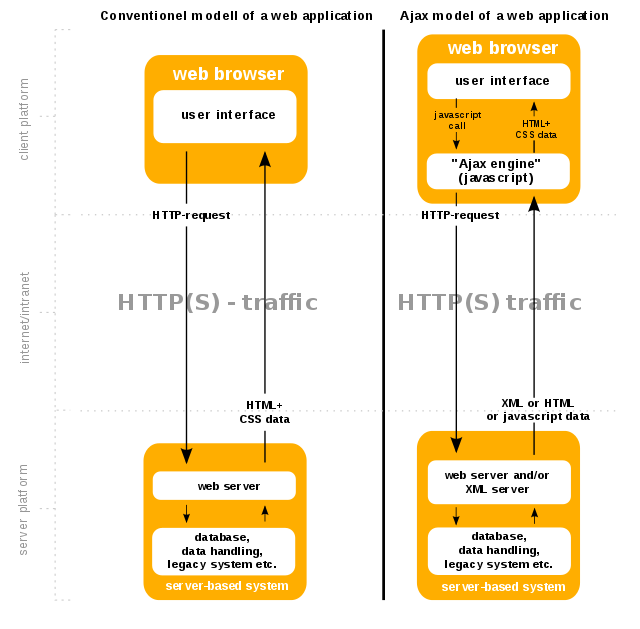
\includegraphics[width=1\textwidth]{./Ajax.png}
	\caption{Conventional method vs \ac{AJAX} method, Source \href{https://en.wikipedia.org/wiki/File:Ajax-vergleich-en.svg}{Wikipedia.com}}
\end{figure}

\ac{AJAX} was greatly utilised in carrying out my projects since most of them exhibited Real-time functionality. Code Snippet 3.1 is a sample snippet from one of the projects with asynchronous data persistence.\\\\\\\\
\begin{code}
	\captionof{listing}{Django Blog's \ac{AJAX} snippet}
	\begin{minted}
	[
	breaklines,
	frame=lines,
	framesep=2mm,
	baselinestretch=1,
	fontsize=\footnotesize,
	linenos
	]
	{JavaScript}
$(document).ready(function(event) {
	$(document).on('submit', '#postcomment', function(event) {
	event.preventDefault();
	$.ajax({
		type: 'POST',
		url: $(this).attr('action'),
		data: $(this).serialize(),
		dataType: 'json',
		success: function(response) {
			$('.comments-wrap').html(response['form']);
				$(document).ready(function() {
					$("#commenters").on("click", ".reply",
					function(event) {
						event.preventDefault();
						var form = $("#postcomment").clone(true);
						form.find('.parent').val($(this)
							.parent().parent().attr('id'));
						$(this).parent().append(form).fade();
				});
			});
			$(document).ready(function() {
				var ssPrettyPrint = function() {
					$('pre').addClass('prettyprint');
					$('code').addClass('prettyprint');
					$(document).ready(function() {
						PR.prettyPrint();
					});
				};
			});
		},
		error: function(rs, e) {
			console.log(rs.responseText);
		},
	})
});
});	
	\end{minted}
\end{code}

The above snippet was the underlying code responsible for the real-time functionality of the Django blog's commenting system. It updates and fetches data from the Comment table which had been created in the blog's models without reloading the entire web page.
\subsection{SQLAlchemy}
According to \citet{Bayer:2016}, The SQLAlchemy \ac{SQL} Toolkit and \ac{ORM} provide a comprehensive set of tools for working with databases and Python. It consists of several distinct areas of functionality which can be individually or collaboratively used together. Below is the illustration of the major components of SQLAlchemy, with component dependencies organized into layers:
\begin{figure}[htbp]
	\centering
	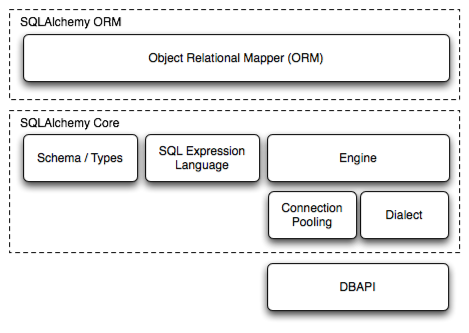
\includegraphics[width=1\textwidth]{./sqlalchemy.png}
	\caption{SQLAlchemy overview, from \citet{Bayer:2016}}
\end{figure}


From the above figure, the two most significant front-facing portions of SQLAlchemy are the \ac{ORM} and the \ac{SQL} Expression Language. SQL Expressions can be used independently of the \ac{ORM}. When using the \ac{ORM}, the \ac{SQL} Expression language remains part of the public facing \ac{API} as it is used within object-relational configurations and queries, \citet{Bayer:2016}.
\subsection{\href{http://jinja.pocoo.org/}{Jinja2}}
\href{http://jinja.pocoo.org/}{Jinja2} is a fast, expressive, extensible and modern day web templating language or engine for Python developers mimicking \ac{DTL} with the inclusion of call functions with arguments on objects. From \citet{Ronacher:2017}, An important usage of Jinga2 is the creation of \ac{HTML}, \ac{XML} or other markup formats which are returned to the user via \ac{HTTP} response.
\section{Python-based Projects}
\subsection{Methodology}
All the web applications were built using Flask or Django framework at the Back-end and Creative Tim’s dashboard and other extensible templates at the front-­end following the procedures below:
\subsubsection{Created the Database tables}
To get started, a back-end of the system which is the database was created. It should be noted that implementing this system was framework dependent as discussed below.
\begin{itemize}
	\item \textbf{Flask}: One of the notable tables in the database was the User table which was created by writing a Class that inherited from Flask's model class. A snippet is:

	\begin{code}
	\captionof{listing}{\ac{vCPE} Flask User Model}
	\begin{minted}
		[
		breaklines,
		frame=lines,
		framesep=2mm,
		baselinestretch=1,
		fontsize=\footnotesize,
		linenos
		]
	{python}
from app         import db
from flask_login import UserMixin

from . common    import COMMON, STATUS, DATATYPE

class User(UserMixin, db.Model):

	id          = db.Column(db.Integer,     primary_key=True)
	user        = db.Column(db.String(64),  unique = True)
	email       = db.Column(db.String(120), unique = True)
	name        = db.Column(db.String(500))
	role        = db.Column(db.Integer)
	password    = db.Column(db.String(500))
	password_q  = db.Column(db.Integer)

	def __init__(self, user, password, name, email):
		self.user       = user
		self.password   = password
		self.password_q = DATATYPE.CRYPTED
		self.name       = name
		self.email      = email
		self.group_id = None
		self.role     = None

	def __repr__(self):
		return '<User %r>' % (self.id)

	def save(self):

		# inject self into db session    
		db.session.add ( self )

		# commit change and save the object
		db.session.commit( )

		return self 
	\end{minted}
	\end{code}
	This piece of code creates a table called \texttt{User} which stores the user information. The table has seven columns: \texttt{id}, a primary key; \texttt{user}  which corresponds to \texttt{User}'s username; \texttt{email} corresponding to \texttt{User}'s email; \texttt{name} corresponding to the name of the \texttt{User}; role; \texttt{password} and \texttt{password\_q} corresponding to the password and confirm password fields of the \texttt{User}. There are also the \texttt{\_\_init\_\_}(Python's Object constructor), \texttt{\_\_repr\_\_}, and \texttt{save} methods all taking \texttt{\textit{"self"}} as an argument, a requirement in Python programming language for methods. \texttt{\_\_init\_\_} and \texttt{\_\_repr\_\_} are called \textit{dunder} or Double Under(Underscores) methods which are sometimes referred to as Magic methods. When an object of the class \texttt{User} is created, the \texttt{\_\_init\_\_} method is invoked while \texttt{\_\_repr\_\_} and its counterpart, \texttt{\_\_str\_\_}, found in Code Snippet 3.2 line 31, controls the \texttt{to-string} conversion in the class that houses it.

	
	Flask uses \texttt{SQLAlchemy} for the \ac{ORM} or Data Access part. It takes charge of the database management such as creating tables, writing \ac{SQL} queries and other database operations. 
	
	
	\item \textbf{Django}: For Django, creation of tables is fairly more verbose but simple. The snippet below buttresses this point.
		\begin{code}
		\captionof{listing}{Django Blog's PublishedManager, Category,and Post}
	\begin{minted}
		[
		breaklines,
		frame=lines,
		framesep=2mm,
		baselinestretch=1,
		fontsize=\footnotesize,
		linenos	
		]
		{python}
from django.contrib.postgres.fields import ArrayField
from django.db import models
from django.contrib.contenttypes.models import ContentType
from django.contrib.auth.models import User
from ckeditor_uploader.fields import RichTextUploadingField
from ckeditor.fields import RichTextField
from django.utils import timezone
from django.urls import reverse
from django.db.models.signals import pre_save
from PIL import Image
from taggit.managers import TaggableManager
from .utils import get_read_time
from django.utils.safestring import mark_safe
#from django.contrib.contenttypes.fields import GenericRelation
		
# Create your models here.
		
class PublishedManager(models.Manager): 
	def get_queryset(self): 
		return super(PublishedManager, self).get_queryset()
		.filter(status='published')
		
class Category(models.Model):
	name = models.TextField(max_length=1000000)
	slug = models.SlugField(max_length=10000000, unique=True)
		
	class Meta:
		ordering = ('name',)
		verbose_name='category'
		verbose_name_plural = 'categories'
		
	def __str__(self):
		return self.name
		
class Post(models.Model):
	STATUS_CHOICES = ( 
		('draft', 'Draft'), 
		('published', 'Published'), 
	) 
	title   = models.CharField(max_length=10000000) 
	slug    = models.SlugField(max_length=10000000, unique_for_date='publish') 
	author  = models.ForeignKey(User, on_delete=models.CASCADE,
	related_name='blog_posts')
	image   = models.ImageField(upload_to='posts_pics'
	,default='logo.svg')
	body    = RichTextUploadingField()
	publish = models.DateTimeField(default=timezone.now)
	read_time =  models.IntegerField(default=0)  
	created = models.DateTimeField(auto_now_add=True) 
	updated = models.DateTimeField(auto_now=True) 
	status  = models.CharField(max_length=100
	,choices=STATUS_CHOICES, default='draft') 
	objects = models.Manager() # The default manager. 
	published = PublishedManager() # Our custom manager.
	category = models.ForeignKey(Category, on_delete=models.CASCADE)
	tags = TaggableManager()
	class Meta: 
		ordering = ('-created',) 
		
	def __str__(self): 
		return self.title
		
		
	def get_absolute_url(self):
		return reverse('blog:post_detail',args=[self.publish.year
		, self.publish.month, self.publish.day, self.slug])
		
	def get_next_post(self):
		return self.get_next_by_created()
		
	def get_previous_post(self):
		return self.get_previous_by_created()
		
	def get_markdown(self):
		body = self.body
		return mark_safe(body)
		
	@property
	def get_content_type(self):
		instance = self
		content_type = ContentType.objects.get_for_model(instance.__class__)
		return content_type
		
	def save(self, *args, **kwargs):
		super(Post, self).save(*args, **kwargs)
		
		img = Image.open(self.image.path)
		width = 883
		height = 391
		if img.width > width or img.height > height:
			output_size = (width, height)
			img.thumbnail(output_size)
			img.save(self.image.path)
	\end{minted}
\end{code}
\end{itemize}
\subsubsection{Created the User Interface}
Although the Database, where tables of any kind could be updated using Django and/or Flask models, had been created, it would be a disaster for users and the technical maintenance team if end users are allowed to manipulate the data directly. Therefore, nice and responsive user interfaces were created to let users interact with the data indirectly. As discussed above, Flask and Django provide templating components to create the user interfaces. Since Flask solely uses \href{http://jinja.pocoo.org/}{Jinja2} whereas Django has an optional \ac{DTL}, the syntax for creating the user interfaces are a bit different.
\begin{itemize}
	\item \textbf{Django}: Django supports two templating engines, namely \href{http://jinja.pocoo.org/}{Jinja2} and \ac{DTL} where the latter happens to be the default with the below snippet.
	\begin{code}
		\captionof{listing}{Django Blog's \texttt{post\_form.html}}
		\begin{minted}
			[
			breaklines,
			frame=lines,
			framesep=2mm,
			baselinestretch=1,
			fontsize=\footnotesize,
			linenos
			]
			{htmldjango}



<!-- site content
================================================== -->
<div class="s-content content">
	<main class="row content__page">
		<section class="column large-full entry format-standard">
			<div class="content__page-header">
				<h1 class="display-1">
					Write A Post.
				</h1>
			</div> <!-- end content__page-header -->
			<form name="contactForm" id="contactForm" method="post"
			action="" autocomplete="on" enctype="multipart/form-data">
				
				<fieldset>
					
						<div class="form-field">
							{{ form.media }}
							{{ field.label }}
							{{ field }}
						</div>
					
					<input name="submit" id="submit" class="btn
					btn--small" value="Create Post" type="submit">
				</fieldset>
			</form> <!-- end form -->
		</section>
	</main>
</div> <!-- end s-content -->

		\end{minted}
	\end{code}
Every line surrounded by \mintinline{htmldjango}{} is a Django sentence which deals with simple \mintinline{htmldjango}{}, \mintinline{htmldjango}{} and \mintinline{htmldjango}{} among others. The lines surrounded by double curly braces, such as \mintinline{htmldjango}{{{ field }}}, denote variables whose values are passed from view functions whenever this template has to be displayed.

	\item \textbf{Flask}: For flask, \href{http://jinja.pocoo.org/}{Jinja2} is one of the major dependencies needed to get it up and running and the syntax looks as follows:
	\begin{code}
		\captionof{listing}{CEA Dashboard \texttt{login.html}}
		\begin{minted}
[
breaklines,
frame=lines,
framesep=2mm,
baselinestretch=1,
fontsize=\footnotesize,
linenos
]
{html+jinja}
<!DOCTYPE html>
<html lang="en">
<head>
<meta charset="UTF-8">
<meta name="viewport" content="width=device-width, initial-scale=1">

	<title>ipNX dashboard - {{ title }}</title>

	<title>ipNX dashboard</title>

</head>
<body>
	<div class="limiter">
		<div class="container-login100">
			<div class="wrap-login100">
				<form class="login100-form validate-form"
				method="POST" action="">
					{{ form.hidden_tag() }}
					<span class="login100-form-logo">
						<img
							src="/static/assets/custom/login
							/images/logo.png" alt="">
					</span>
					<span class="login100-form-title p-b-34 p-t-27">
						Log in
					</span>
					
						<div class="text-center p-t-5 p-b-5">
							<p class="error">
								{{ message }}
							</p>      
						</div>
					
					<div class="wrap-input100 validate-input"
					data-validate="Enter E-mail">
						{{ form.email(class="input100",
							placeholder="E-mail") }}
						<span class="focus-input100"
							data-placeholder="&#xf207;">
						</span>
					</div>
			
					<div class="wrap-input100 validate-input"
					data-validate="Enter password">
						{{ form.password(placeholder="Password",
							class="input100") }}
							<span class="focus-input100"
								data-placeholder="&#xf191;">
							</span>
					</div>
			
					<div class="contact100-form-checkbox">
						{{ form.remember(class="input-checkbox100",
							id="ckb1",type="checkbox") }}
						<label class="label-checkbox100" for="ckb1">
							Remember me
						</label>
					</div>
			
					<div class="container-login100-form-btn">
			
						{{ form.submit(class="login100-form-btn") }}
			
					</div>
			
					<div class="text-center p-t-10">
						<a class="txt1" href="#">
							Forgot Password?
						</a>
					</div>
				</form>
			</div>
		</div>
	</div>
			
</body>
			
</html>
		\end{minted}
	\end{code}
\end{itemize}
\subsection{Implemented the view function}
Having dealt with the back-end databases and the frontend web pages user interfaces, the logic which stands in between to deal with the user requests and maintain the database were implemented. Unsurprisingly, the view systems in Flask and Django are different.
\begin{itemize}
	\item \textbf{Django}: Django's views component provides a set of \ac{API} to implement the logic. The Django view file, \texttt{views.py}, houses the functions and/or classes to achieve all set goals. The view functions and/or classes are shown in the snippet below:
	\begin{code}
		\captionof{listing}{Django's Blog \texttt{views.py}}
		\begin{minted}
[
breaklines,
frame=lines,
framesep=2mm,
baselinestretch=1,
fontsize=\footnotesize,
linenos
]
{python}
from django.shortcuts import render, get_object_or_404, redirect
from django.contrib.contenttypes.models import ContentType
from django.template.defaultfilters import slugify
from django.http import HttpResponse, HttpResponseRedirect, 
Http404, JsonResponse
from django.core.paginator import Paginator, 
EmptyPage, PageNotAnInteger
from django.views import generic
from django.contrib.auth.mixins import LoginRequiredMixin
, UserPassesTestMixin

from taggit.models import Tag
from django.contrib.auth.decorators import login_required
from django.db.models import Count, Q
from django.contrib.auth.models import User
from .models import Post, Comment
from .forms import PostForm, UpdatePostForm, CommentForm
from django.template.loader import render_to_string
from django.contrib.postgres.search import SearchVector, 
SearchQuery, SearchRank, TrigramSimilarity

#Function based view
def blog_index(request, tag_slug=None):
	object_list = Post.published.all()
	if request.user.is_staff or request.user.is_superuser:
		object_list = Post.objects.all()
	common_tags = Post.tags.most_common()[:2]
	tag = None

	if tag_slug:
		tag = get_object_or_404(Tag, slug=tag_slug)
		object_list = object_list.filter(tags__in=[tag])

	paginator = Paginator(object_list, 5) # 5 posts in each page
	page = request.GET.get('page')
	try:
		posts = paginator.page(page)
		except PageNotAnInteger:
		# If page is not an integer deliver the first page
		posts = paginator.page(1)
	except EmptyPage:
		# If page is out of range deliver last page of results
		posts = paginator.page(paginator.num_pages)
	context = {
		'page': page, 
		'posts': posts, 
		'tag': tag, 
		'common_tags': common_tags,
	}
	return render(request, 'blog/index.html', context)
	
#Class based view
class PostUpdateView(LoginRequiredMixin, 
		UserPassesTestMixin, generic.UpdateView):
	model = Post
	form_class=UpdatePostForm
	template_name = 'blog/post_form.html'

	def form_valid(self, form):
		form.instance.author = self.request.user
		return super().form_valid(form)

	def test_func(self):
		post = self.get_object()
	if self.request.user == post.author or self.request.user.is_staff:
		return True
	return False
		\end{minted}
	\end{code}
	\item \textbf{Flask}: According to \citet{Grinberg:2014}, "Clients such as web browsers send requests to the web server, which in turn sends them to the Flask application instance. The application instance needs to know what code needs to run for each URL requested, so it keeps a mapping of URLs to Python functions. The association between a URL and the function that handles it is called a \texttt{route}. The most convenient way to define a route in a Flask application is through the \texttt{app.route} decorator exposed by the application instance, which registers the decorated
	function as a \texttt{route}. The following example shows how a route is declared using this decorator:
	\begin{code}
		\captionof{listing}{Example snippet}
		\begin{minted}
[
breaklines,
frame=lines,
framesep=2mm,
baselinestretch=1,
fontsize=\footnotesize,
linenos
]
{python}
@app.route('/')
def index():
	return '<h1>Hello World!</h1>'

		\end{minted}
	\end{code}
Functions like index() are called view functions" and are mostly housed in the \texttt{views.py} file and an example of a comprehensive \texttt{views.py} file is shown below:
\begin{code}
	\captionof{listing}{An excerpt from CEA dashboard's \texttt{views.py} file}
	\begin{minted}
[
breaklines,
frame=lines,
framesep=2mm,
baselinestretch=1,
fontsize=\footnotesize,
linenos
]
{python}
# all the imports necessary

from flask import json, url_for, redirect, Markup, 
Response, render_template, flash, g, session, jsonify, 
request, send_from_directory
from werkzeug.exceptions import HTTPException, NotFound, abort

import os
import secrets
from PIL import Image
from app  import app

from flask       import url_for, redirect, render_template, 
flash, g, session, jsonify, request, send_from_directory
from flask_login import login_user, logout_user, 
current_user, login_required
from app         import app, lm, db, bc
from . models    import User
from . common    import COMMON, STATUS
from . assets    import *
from . forms     import LoginForm, RegisterForm, UpdateAccountForm
import os, shutil, re, cgi, json, random, time
from datetime import datetime


random.seed()  # Initialize the random number generator

# provide login manager with load_user callback
@lm.user_loader
def load_user(user_id):
	return User.query.get(int(user_id))
@app.route('/index')
@login_required
def index():
	inactiveCustomers = 34546
	activeCustomers = 7654984
	numberOfCalls = 123456
	numberOfRetailCustomers = 455674666
	return render_template('pages/index.html',
	numberOfCalls=numberOfCalls,
	numberOfRetailCustomers=numberOfRetailCustomers,
	inactiveCustomers=inactiveCustomers,
	activeCustomers=activeCustomers)


# authenticate user
@app.route('/logout')
def logout():
	logout_user()
	return redirect(url_for('login'))
	\end{minted}
\end{code}
\end{itemize}

\subsection{Projects Implemented}
Some of the projects implemented using the Python programming language and its two most popular frameworks, Django and Flask, are undermentioned and discussed.
\subsubsection{Customer Premises Equipment (CPE)}
\begin{itemize}
	\item \textbf{Project's Requirement specification}:
	The project was to "build a web UI for a customer premises equipment (CPE) through which settings can be modified.
	
	Please design such a web UI with the following pages:
	\begin{itemize}
		\item[*] Login page - username and password
		\item[*] Main page - device summary showing WAN and LAN IPv4 addresses
		\item[*] Settings page -
		\subitem Enable/disable DHCP service, modify address range, manage DHCP reservations
		\subitem Manage DNS servers
		\subitem Manage device whitelist/blacklist based on MAC addresses
		\subitem Manage WiFi settings including ESSID name and pre-shared key (password), enable/disable 2.4GHz and/or 5GHz bands, add or remove WiFi devices
	\end{itemize} 
	
	
	This must be a responsive site with a nice UI and interaction. Communication between front-end and back-end should JSON over XHR asynchronously. Backend should be Python or PHP based with data persistence in SQLite on the backend server".
\end{itemize}

Having implemented the features stated using Flask, the system was initiated and Figure 3.3 shows the pages of each feature:
\begin{figure}[!htbp]
	\centering
\begin{subfigure}[b]{0.45\textwidth}
	\centering
	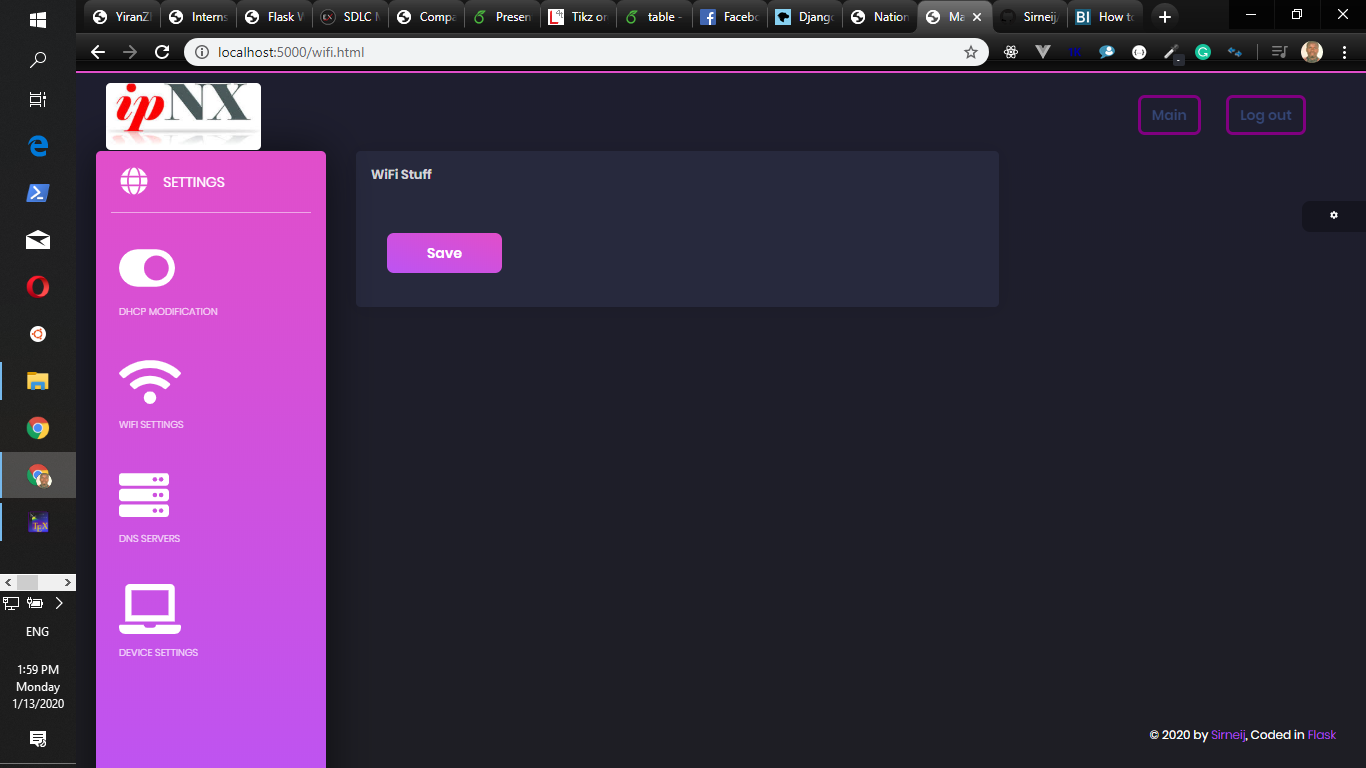
\includegraphics[width=\linewidth]{./vcpewifi}
	\caption{\ac{vCPE} WiFi management page}
\end{subfigure}
\hfill
\begin{subfigure}[b]{0.45\textwidth}
	\centering
	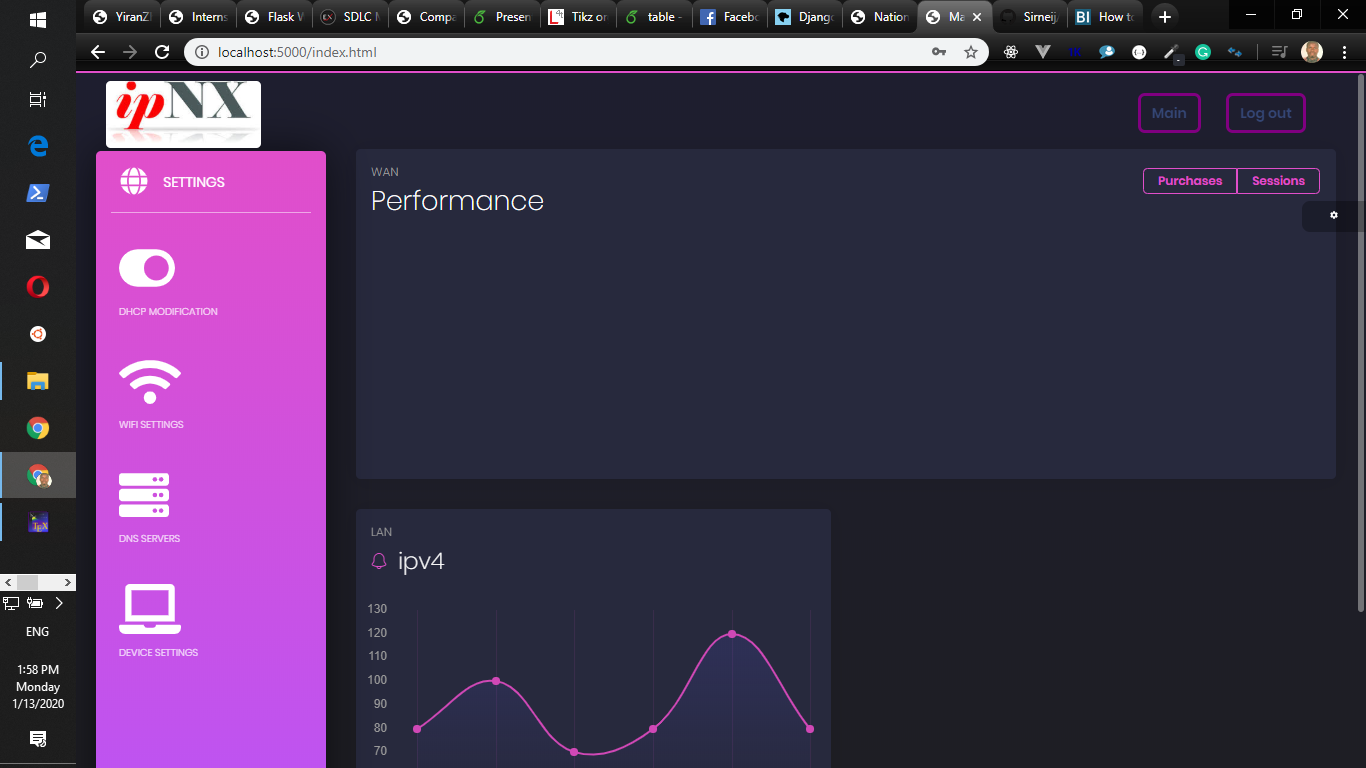
\includegraphics[width=\linewidth]{./vcpemainpage}
	\caption{\ac{vCPE}  Main page}
\end{subfigure}
\medskip
\begin{subfigure}[b]{0.45\textwidth}
	\centering
	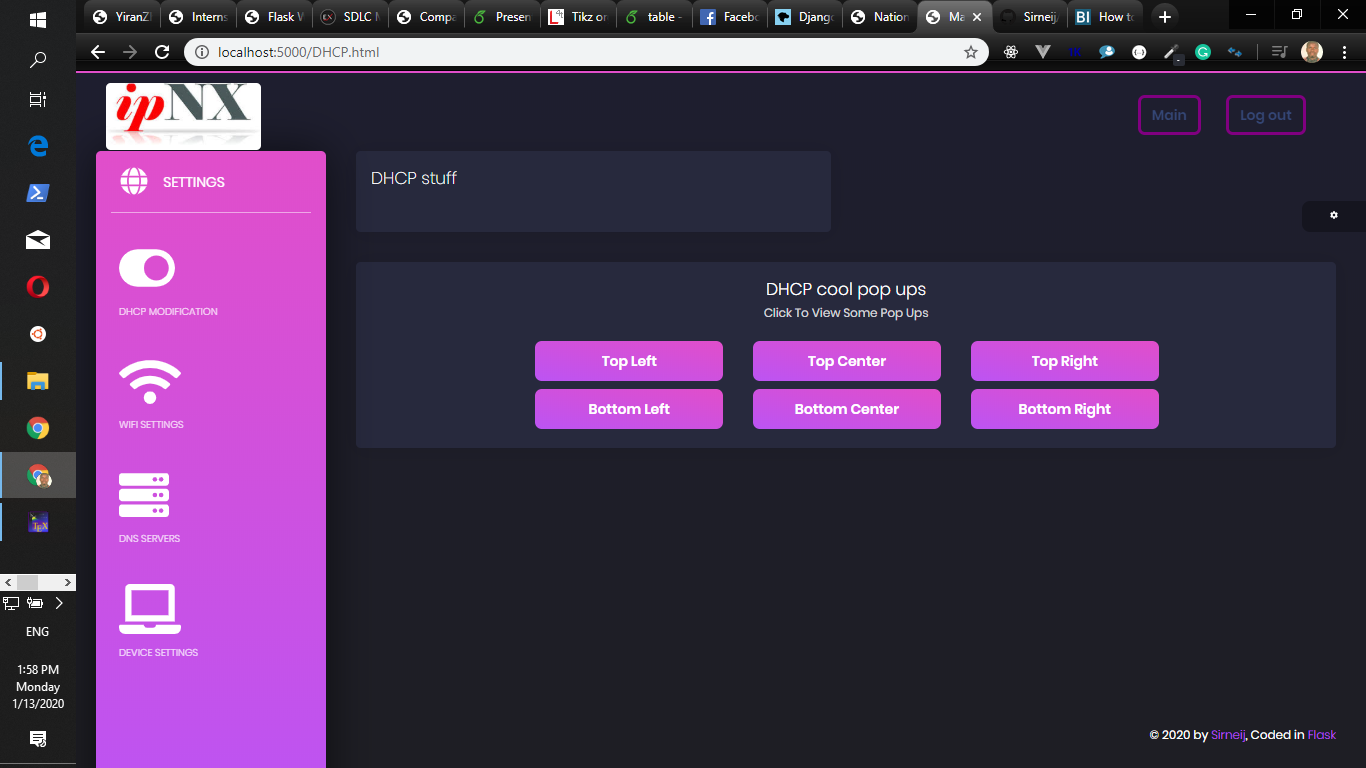
\includegraphics[width=\linewidth]{./vcpedhcp}
	\caption{\ac{vCPE} DHCP page}
\end{subfigure}
\hfill
\begin{subfigure}[b]{0.45\textwidth}
	\centering
	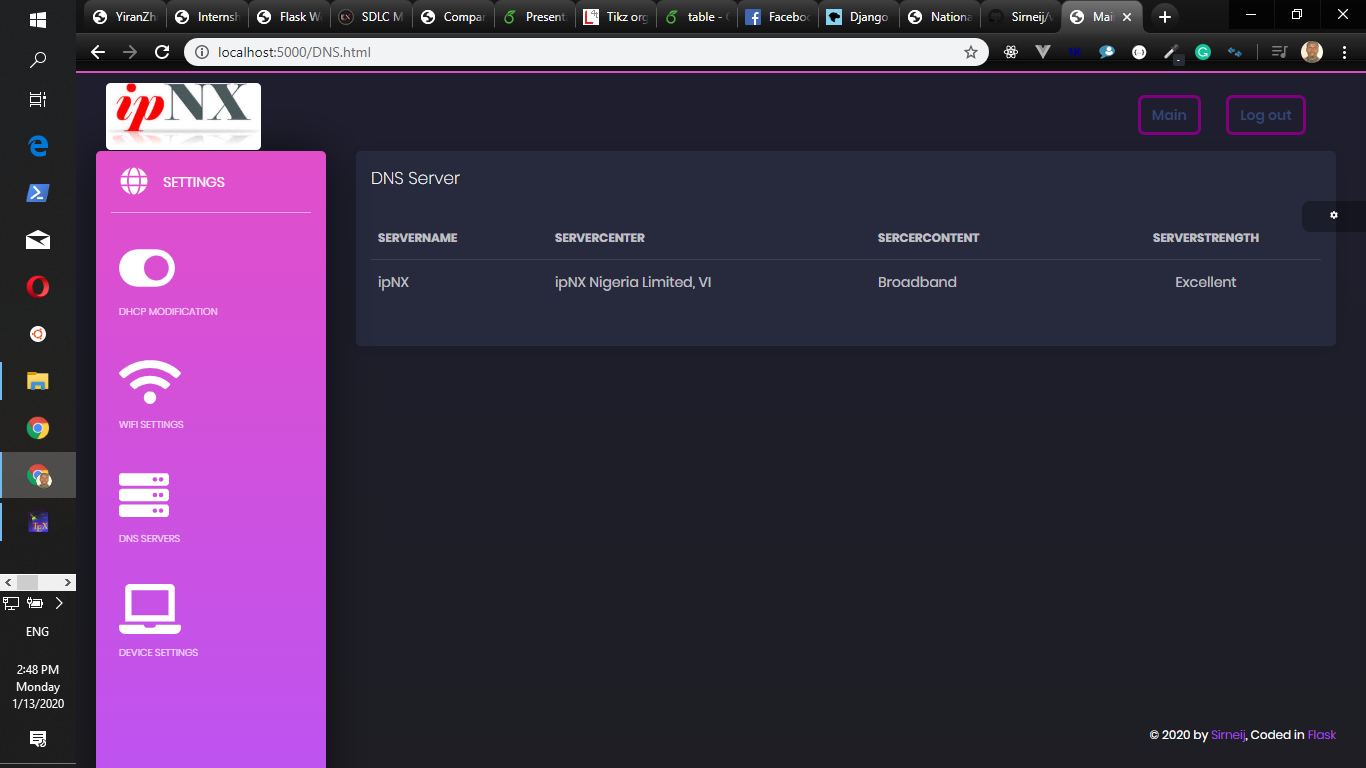
\includegraphics[width=\linewidth]{./vcpednsserver}
	\caption{\ac{vCPE}  DNS Server page}
\end{subfigure}
\medskip
\begin{subfigure}[b]{0.45\textwidth}
	\centering
	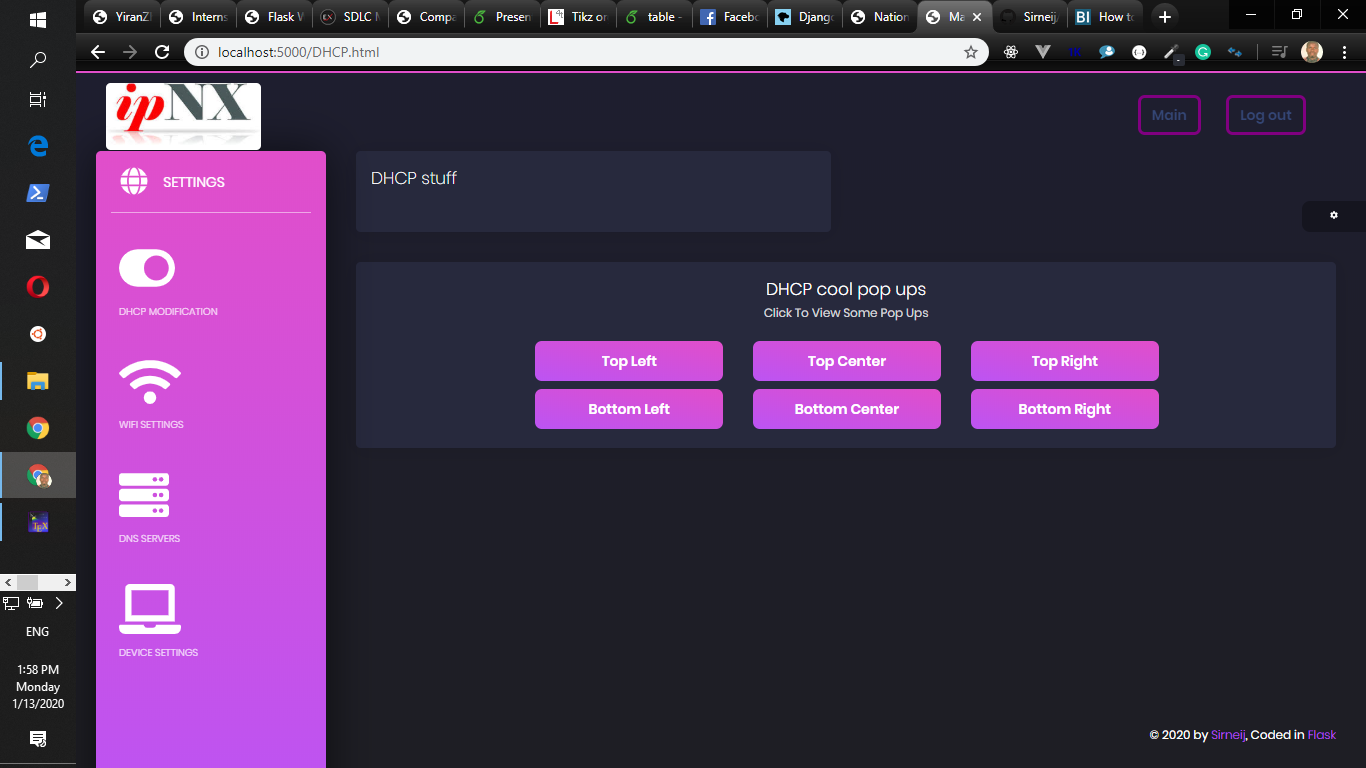
\includegraphics[width=\linewidth]{./vcpedhcp}
	\caption{\ac{vCPE} DHCP page}
\end{subfigure}
\hfill
\begin{subfigure}[b]{0.45\textwidth}
	\centering
	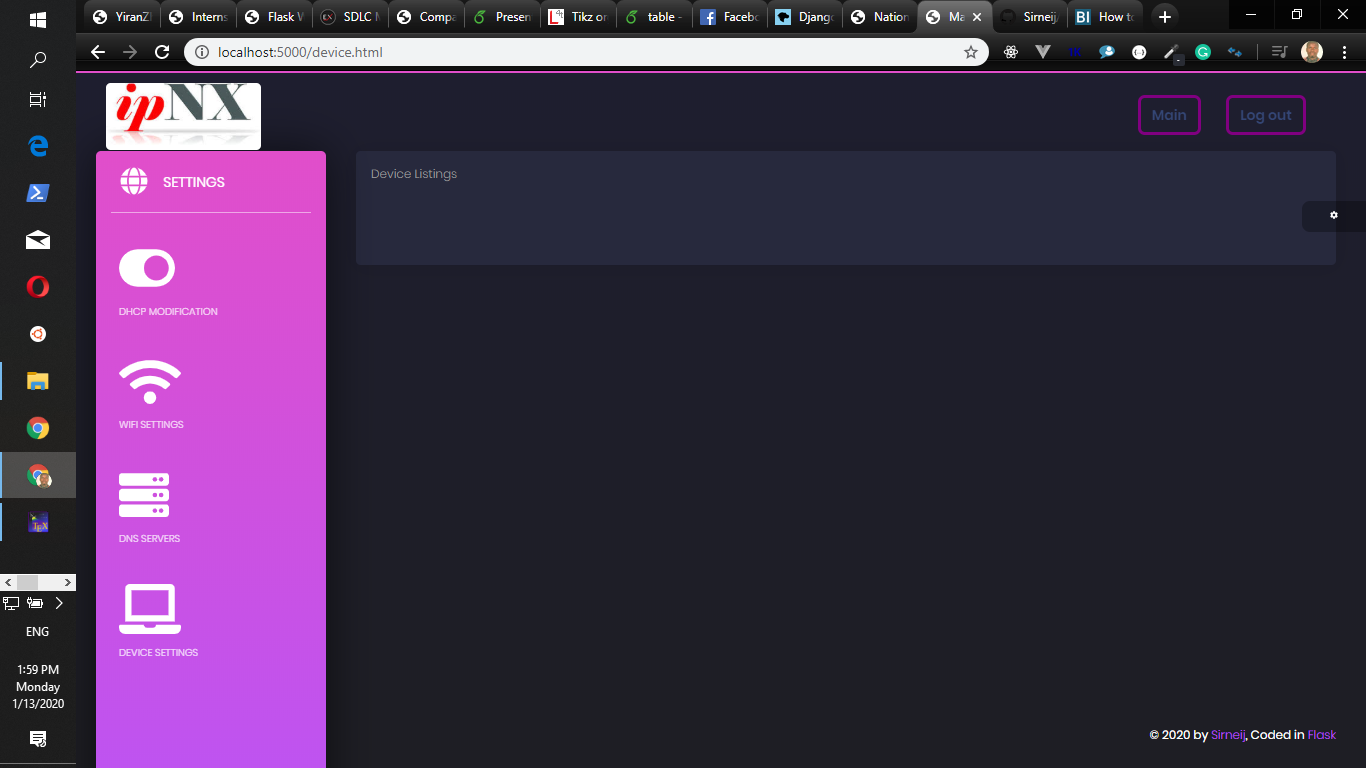
\includegraphics[width=\linewidth]{./vcpedevice}
	\caption{\ac{vCPE}  Devices List page}
\end{subfigure}
\medskip
\begin{subfigure}[b]{0.45\textwidth}
	\centering
	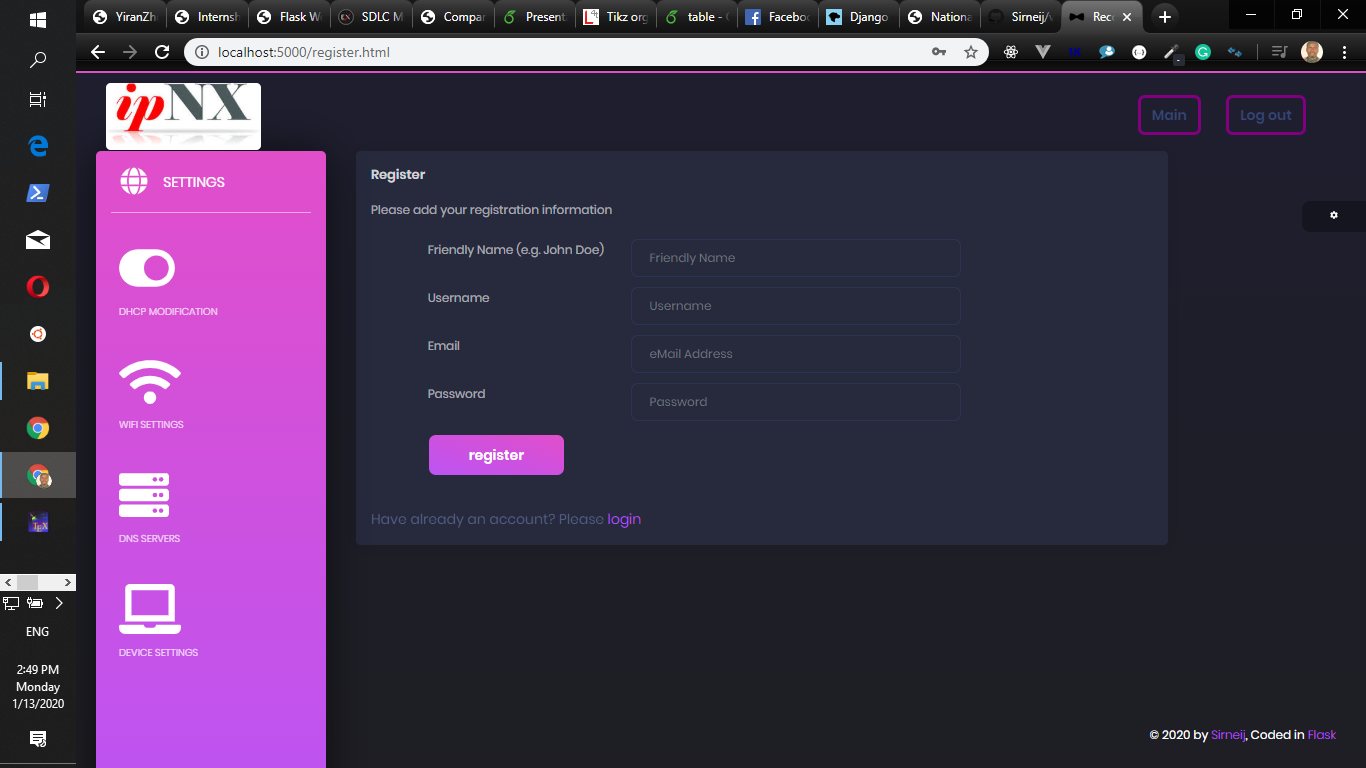
\includegraphics[width=\linewidth]{./vcperegister}
	\caption{\ac{vCPE} Registration page, \textit{restricted to an admin}.}
\end{subfigure}\hfill
\begin{subfigure}[b]{0.45\textwidth}
	\centering
	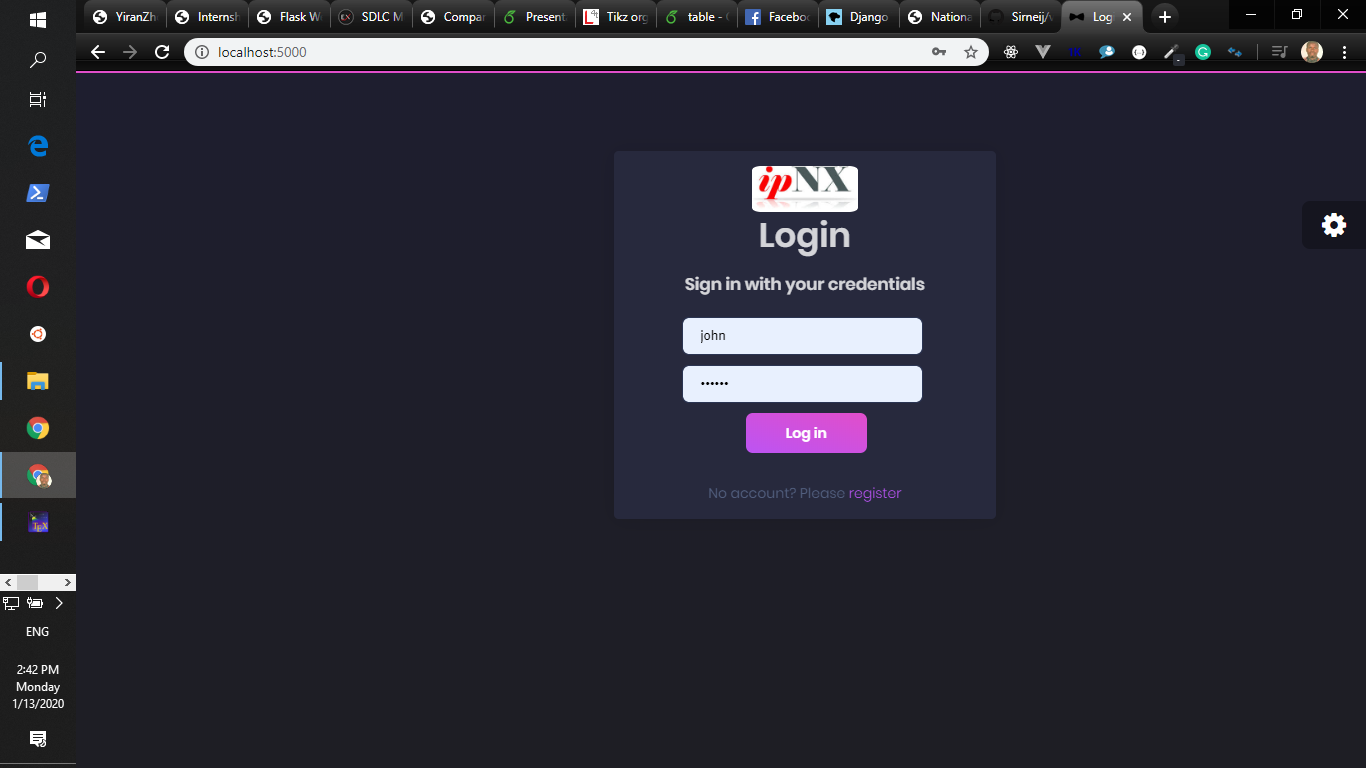
\includegraphics[width=\linewidth]{./vcpelogin}
	\caption{\ac{vCPE} Login page}
\end{subfigure}
	\caption{\ac{vCPE} Screenshots}
\end{figure}
\subsubsection{Customer Experience Analysis (CEA) Dashboard}
\begin{itemize}
	\item \textbf{Project's Requirement specification}: Customer Experience Analysis (CEA) Dashboard's requirement specification was to develop or implement a real-time dashboard which has the metrics and features as shown in the Figure 3.5 below:\\\\\\\\
	\begin{figure}[!htbp]
		\centering
		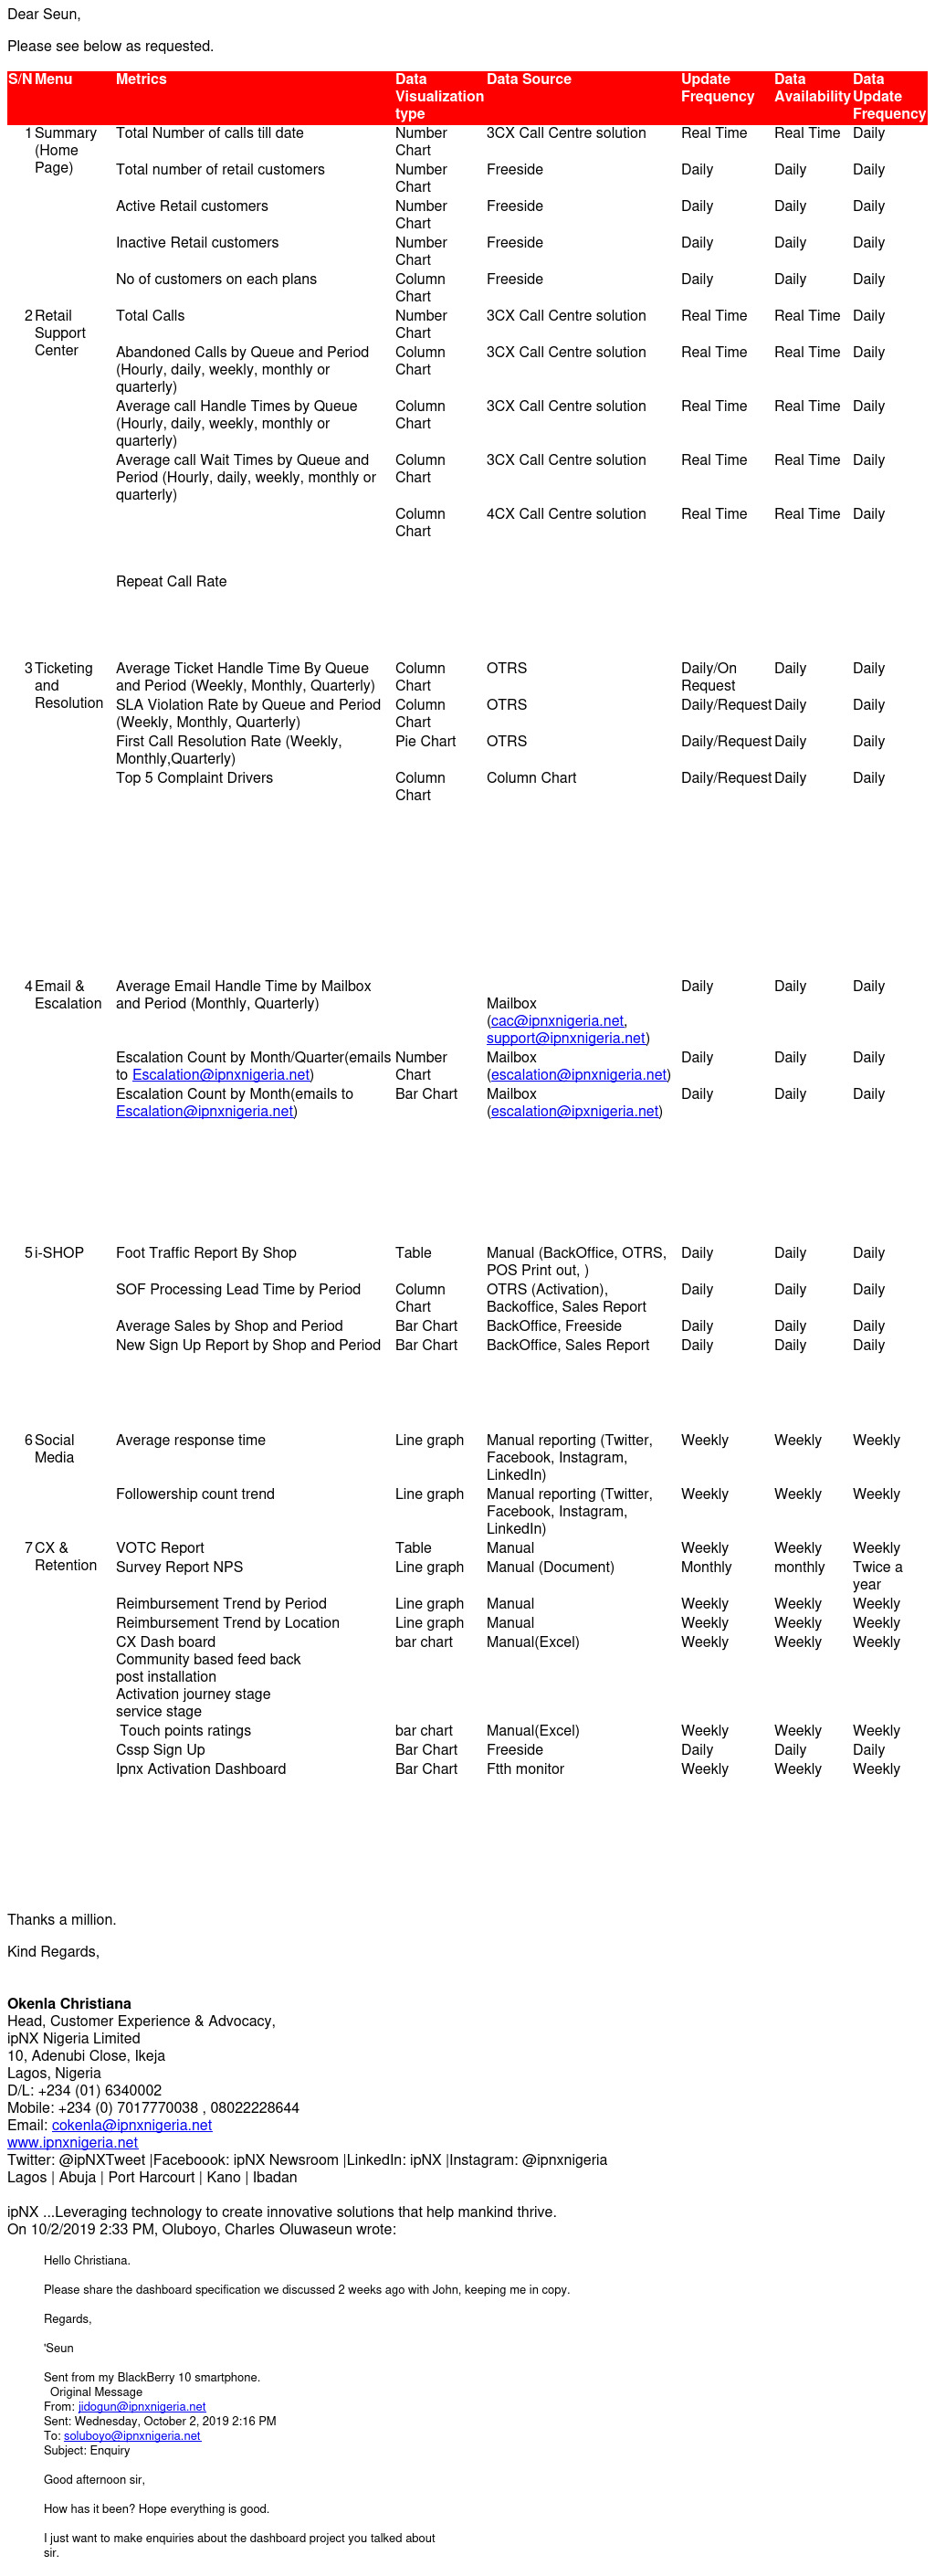
\includegraphics[width=1\linewidth,height=0.9\textheight]{./ceadash}
		\caption{Customer Experience Analysis (CEA) Dashboard specification sent by \textit{ip}NX's Head of Customer Experience \& Advocacy.}
	\end{figure}
	Figure 3.6 depicts the looks of the software product which was wholly implemented in Python's Flask:
	\begin{figure}[!htbp]
		\centering
		\begin{subfigure}[b]{0.45\textwidth}
			\centering
			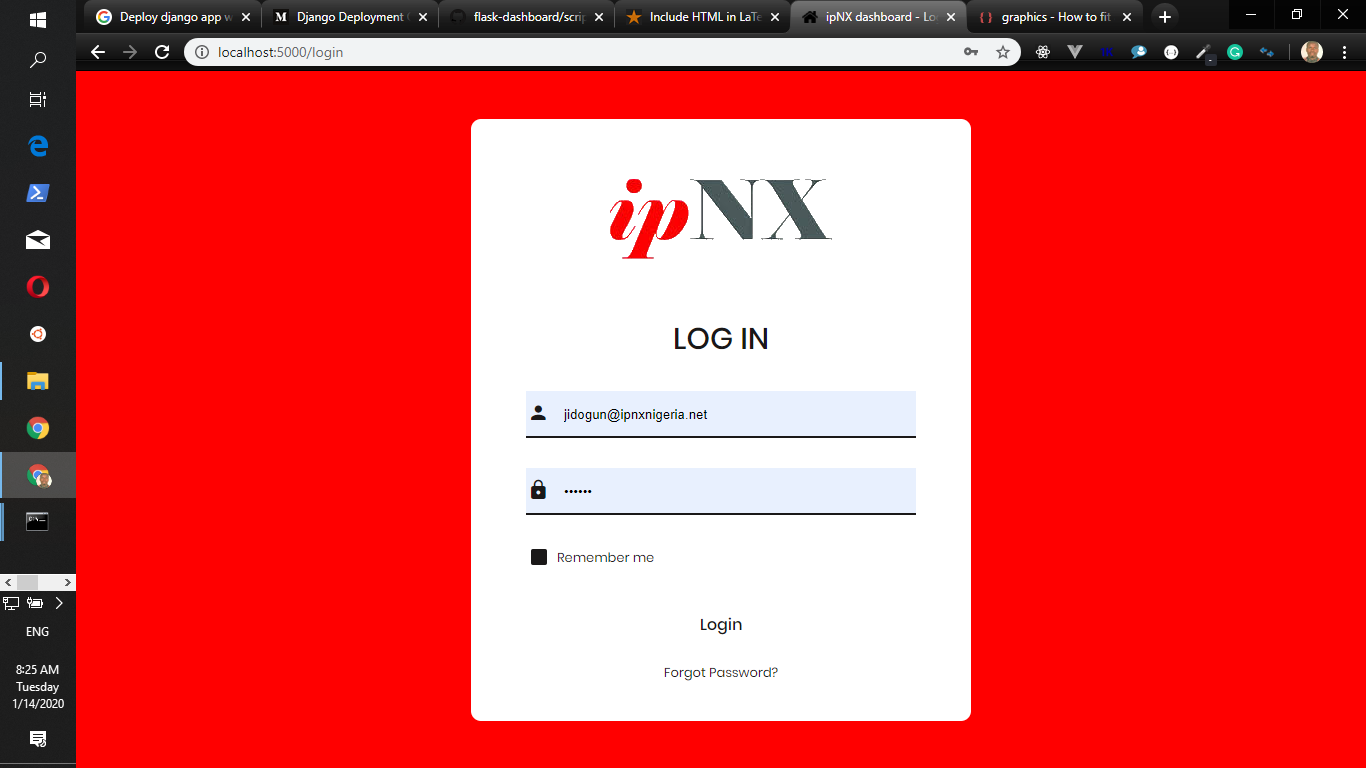
\includegraphics[width=\linewidth]{./cealogin}
			\caption{CEA dashboard Login page}
		\end{subfigure}
		\hfill
		\begin{subfigure}[b]{0.45\textwidth}
			\centering
			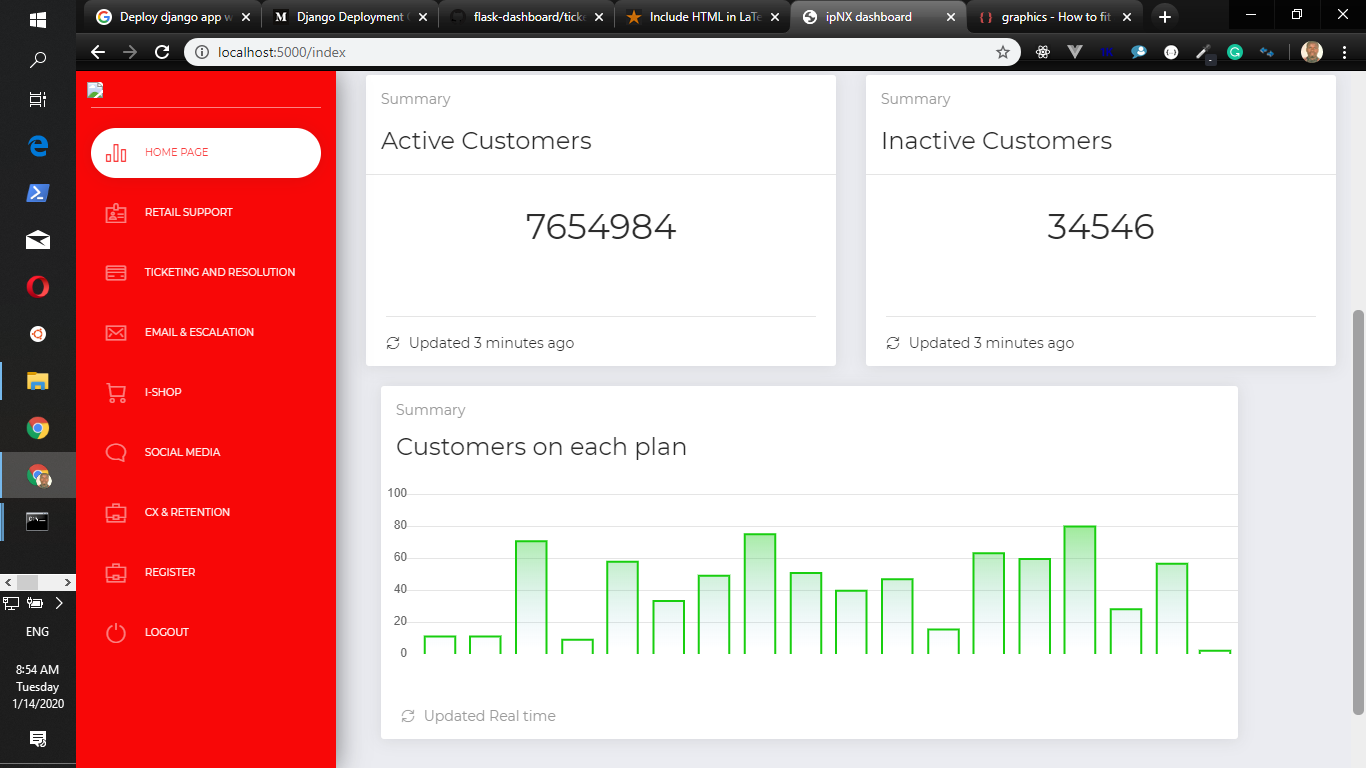
\includegraphics[width=\linewidth]{./ceaindex}
			\caption{CEA dashboard Landing or main page}
		\end{subfigure}
		\medskip
		\begin{subfigure}[b]{0.45\textwidth}
			\centering
			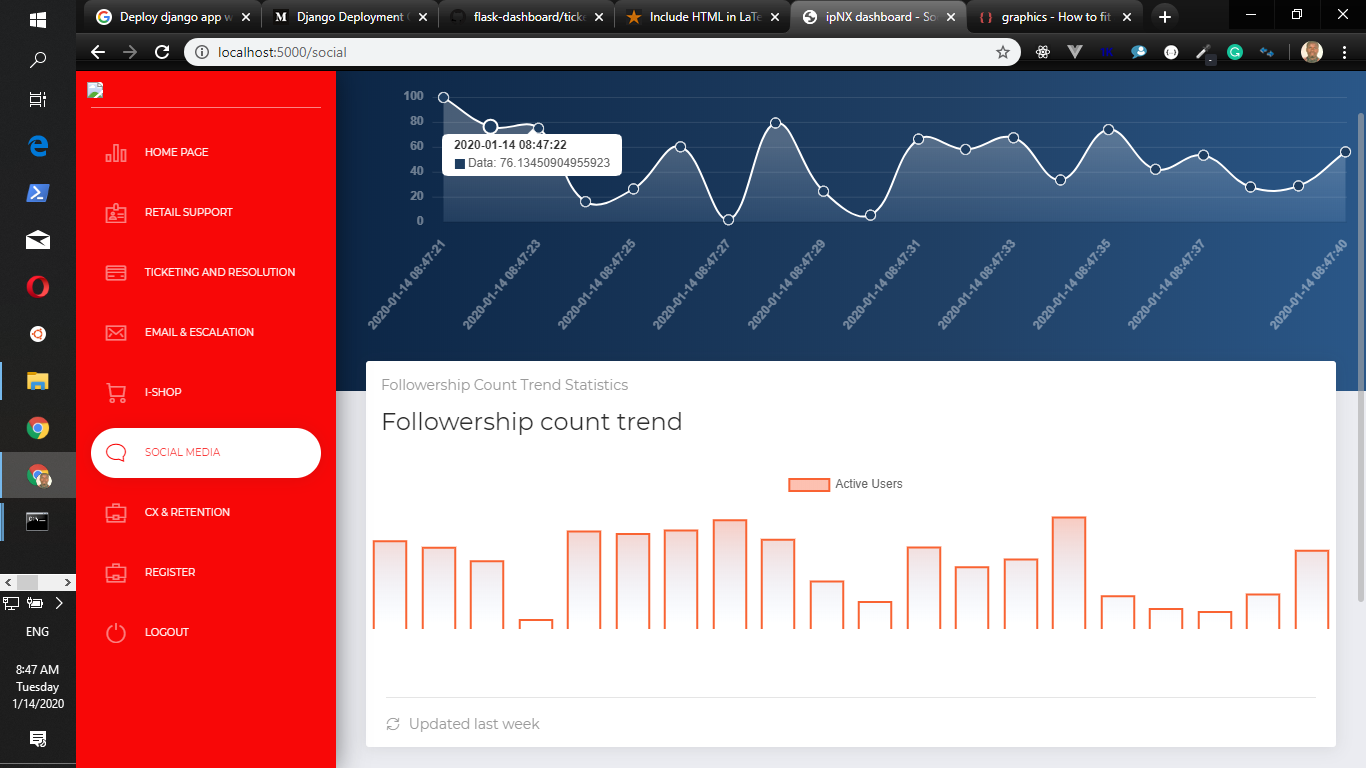
\includegraphics[width=\linewidth]{./ceasocial}
			\caption{CEA dashboard Social menu page}
		\end{subfigure}
		\hfill
		\begin{subfigure}[b]{0.45\textwidth}
			\centering
			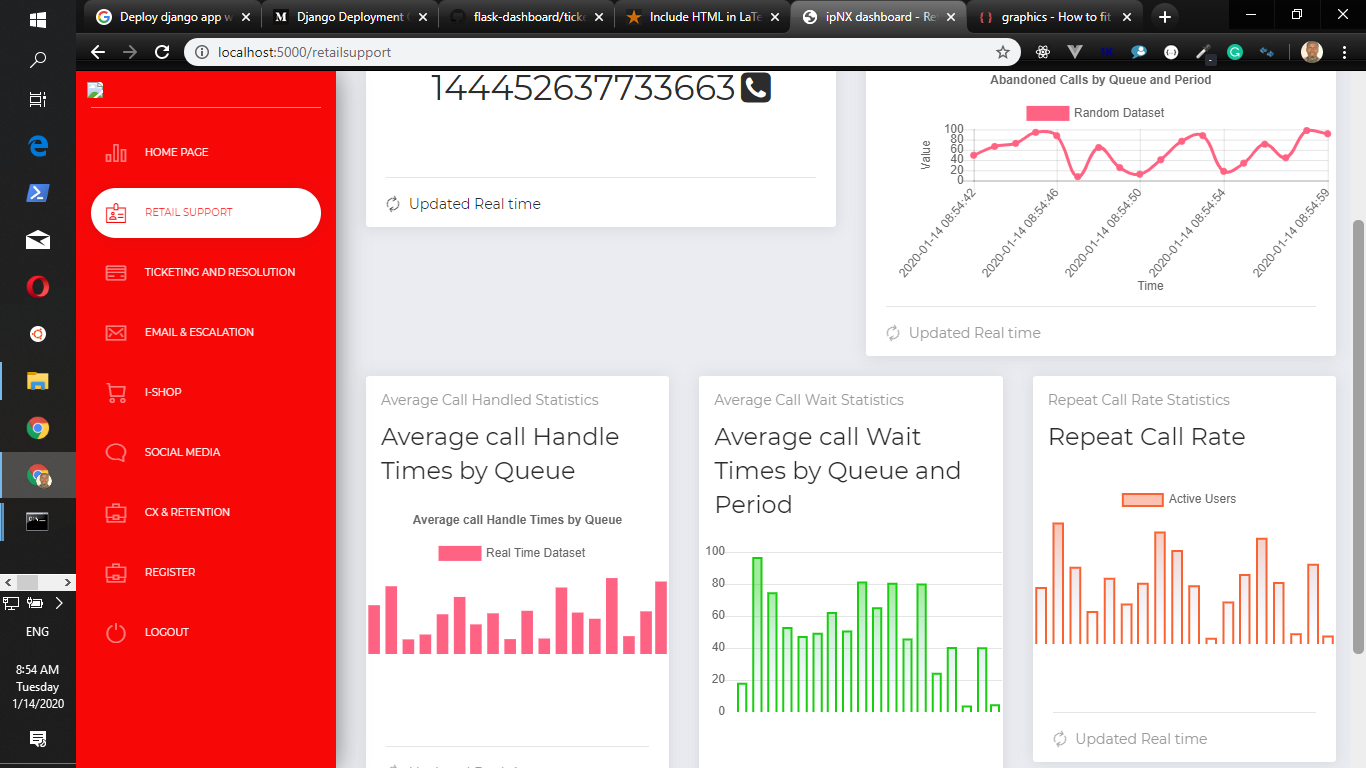
\includegraphics[width=\linewidth]{./cearetail}
			\caption{CEA dashboard Retail menu page}
		\end{subfigure}
		\caption{Some CEA dashboard pages with Real-time data visualization.}
	\end{figure}
\end{itemize}
\subsubsection{Data Usage Analytic (DUA) Dashboard}
\begin{itemize}
	\item \textbf{Project's requirement specification}: \textit{ip}NX already had a Data Usage Analytic (DUA) Dashboard but was with poor design and user interface. The task was to re-engineer, re-develop and revamp the whole system with the following additional features:
	\subitem Animated Error page for advertisement.
	\subitem Modal views of preliminary Data Usage analysis of each device on each user's network.
	\subitem Attractive Login page with company's products advertisement as carousels.
	\subitem Responsive Dashboard theme selection pluggin.\\
	
	
	 Figures 3.7 and 3.8 show the initial system as well as its re-designed, using Flask micro-framework, counterpart.
		\begin{figure}[!htbp]
		\centering
		\begin{subfigure}[b]{0.45\textwidth}
			\centering
			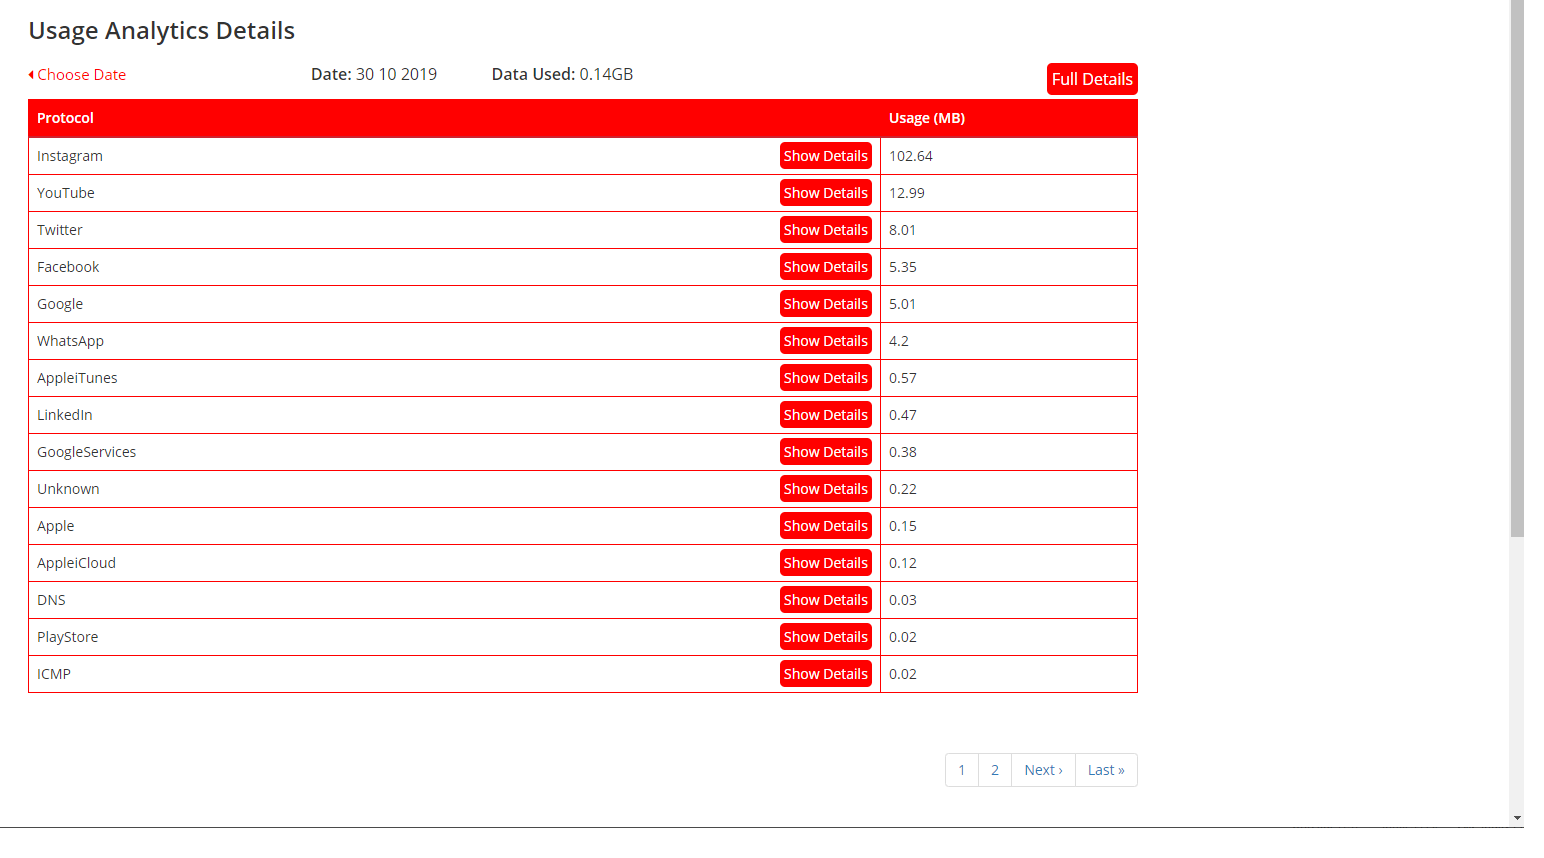
\includegraphics[width=\linewidth]{./duaformeranalytic}
			\caption{DUA dashboard data analytics}
		\end{subfigure}
		\hfill
		\begin{subfigure}[b]{0.45\textwidth}
			\centering
			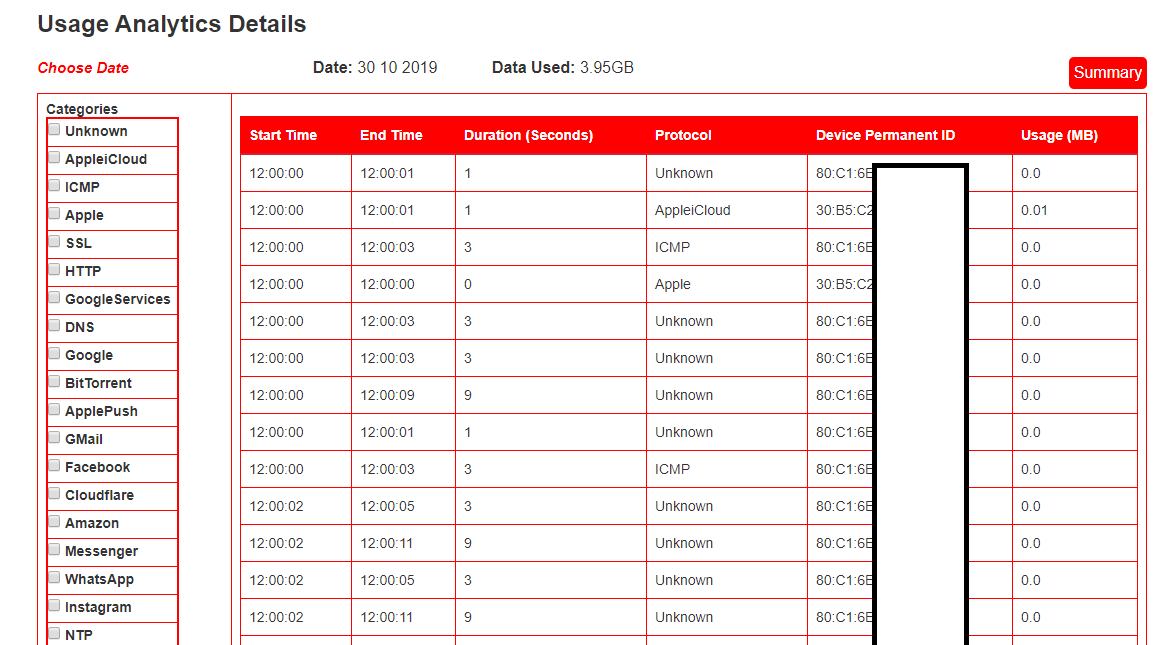
\includegraphics[width=\linewidth]{./duaformeranalyticdetail}
			\caption{DUA dashboard data analytics details}
		\end{subfigure}
		\caption{Former DUA dashboard pages.}
	\end{figure}
	\begin{figure}[!htbp]
		\centering
		\begin{subfigure}[b]{0.45\textwidth}
			\centering
			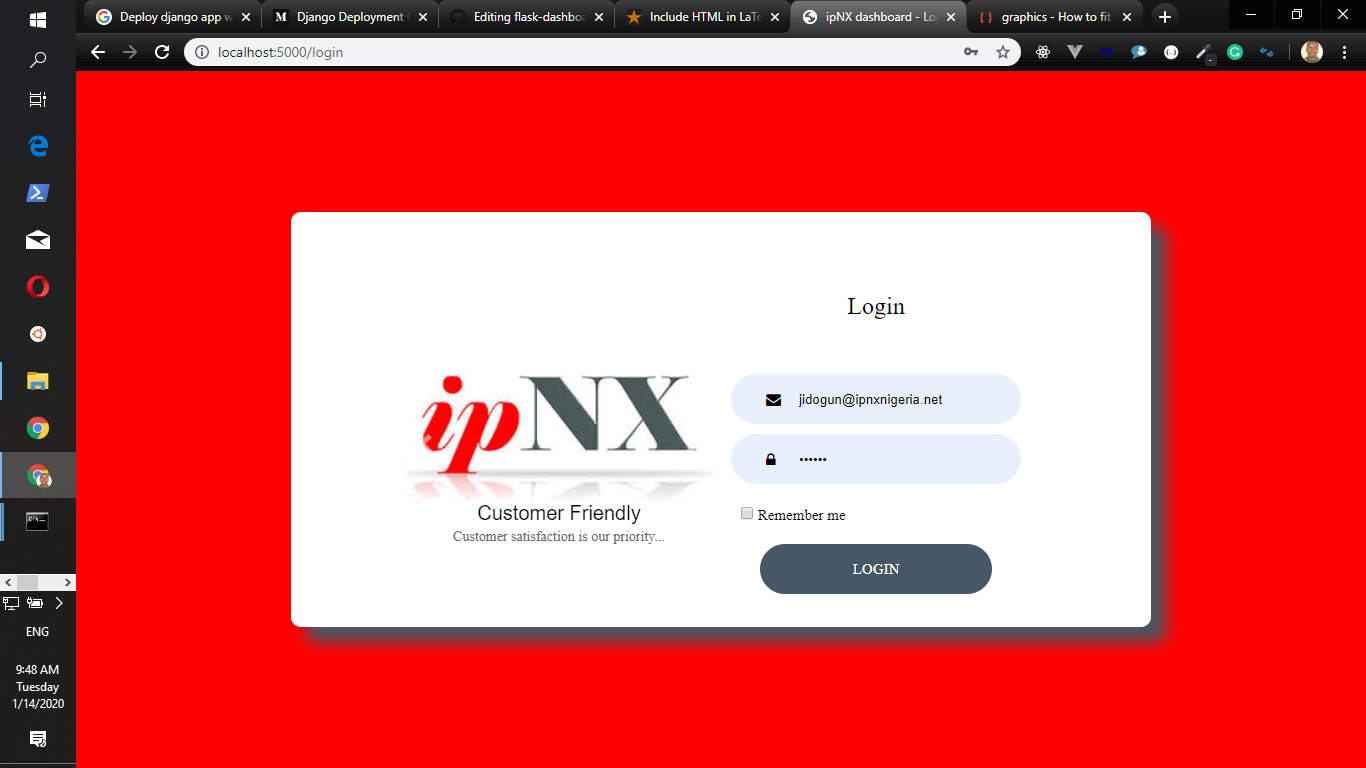
\includegraphics[width=\linewidth]{./dualogin}
			\caption{DUA dashboard Animated Login page}
		\end{subfigure}
		\hfill
		\begin{subfigure}[b]{0.45\textwidth}
			\centering
			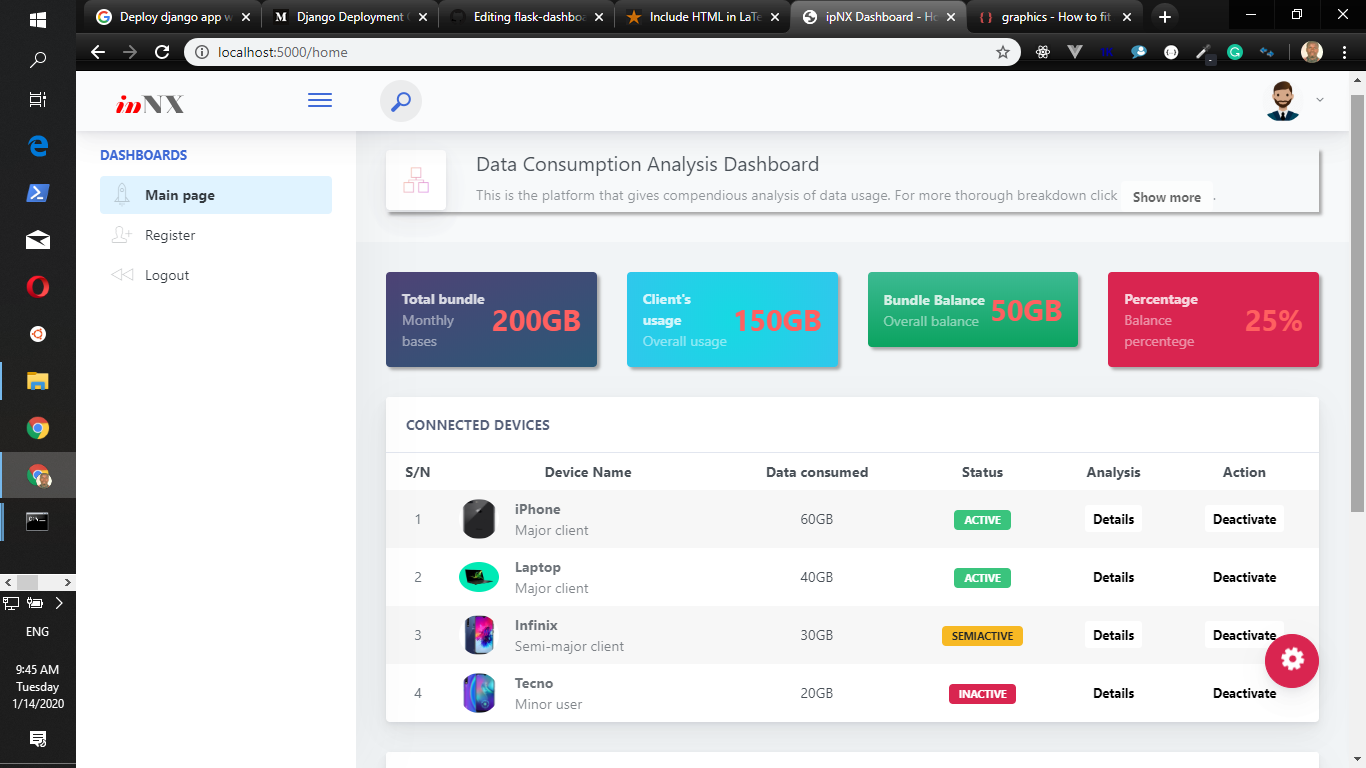
\includegraphics[width=\linewidth]{./duadata}
			\caption{DUA dashboard data analysis page}
		\end{subfigure}
	\medskip
	\begin{subfigure}[b]{0.45\textwidth}
		\centering
		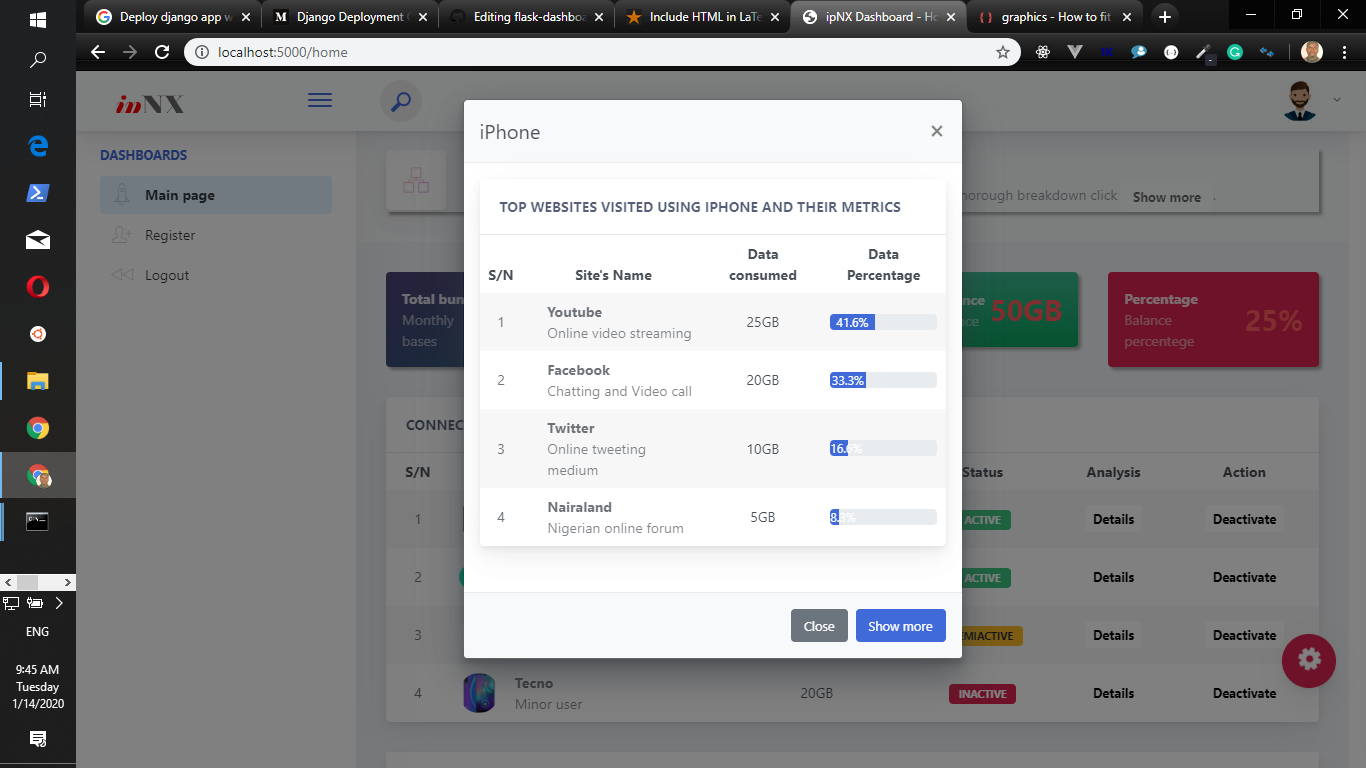
\includegraphics[width=\linewidth]{./duamodal}
		\caption{DUA dashboard modal data analysis page}
	\end{subfigure}
	\hfill
	\begin{subfigure}[b]{0.45\textwidth}
		\centering
		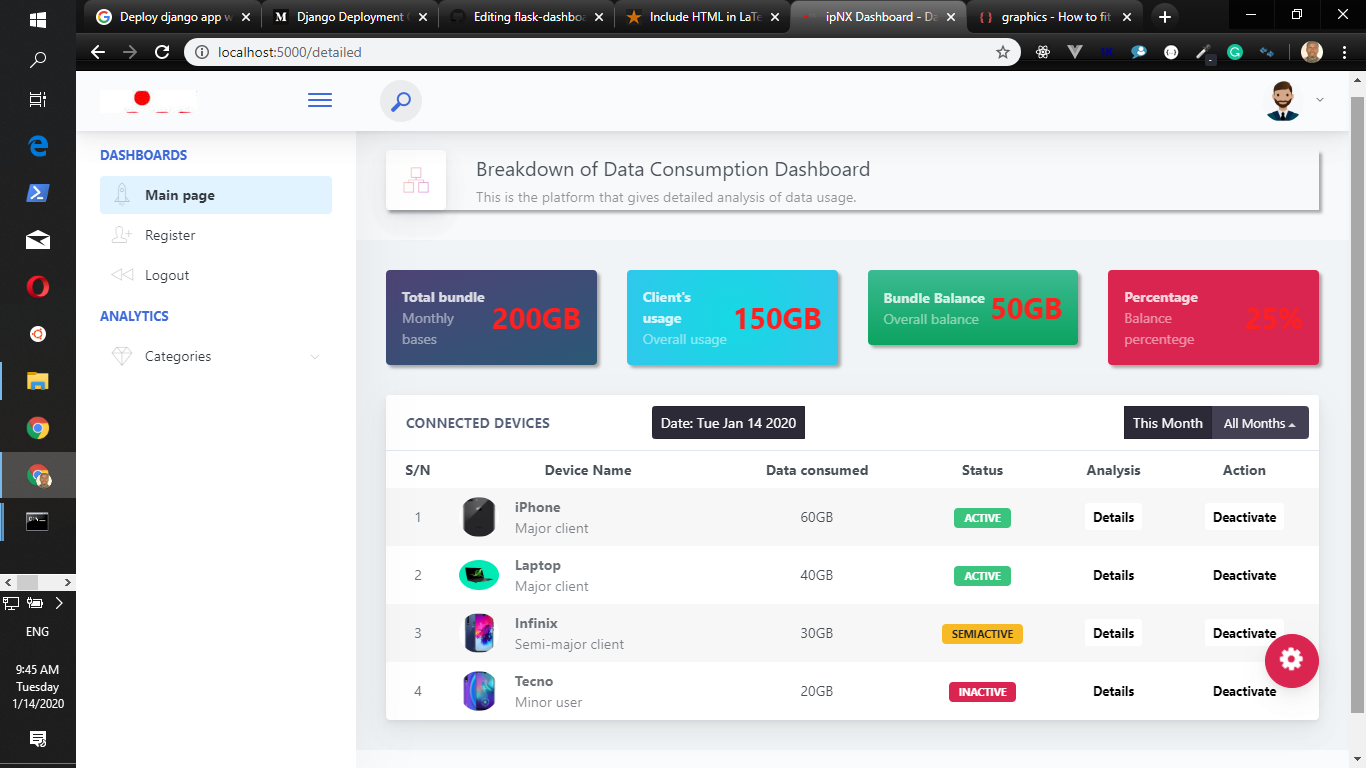
\includegraphics[width=\linewidth]{./duadatadetails}
		\caption{DUA dashboard detailed data analysis page}
	\end{subfigure}
	\medskip
	\begin{subfigure}[b]{0.5\textwidth}
		\centering
		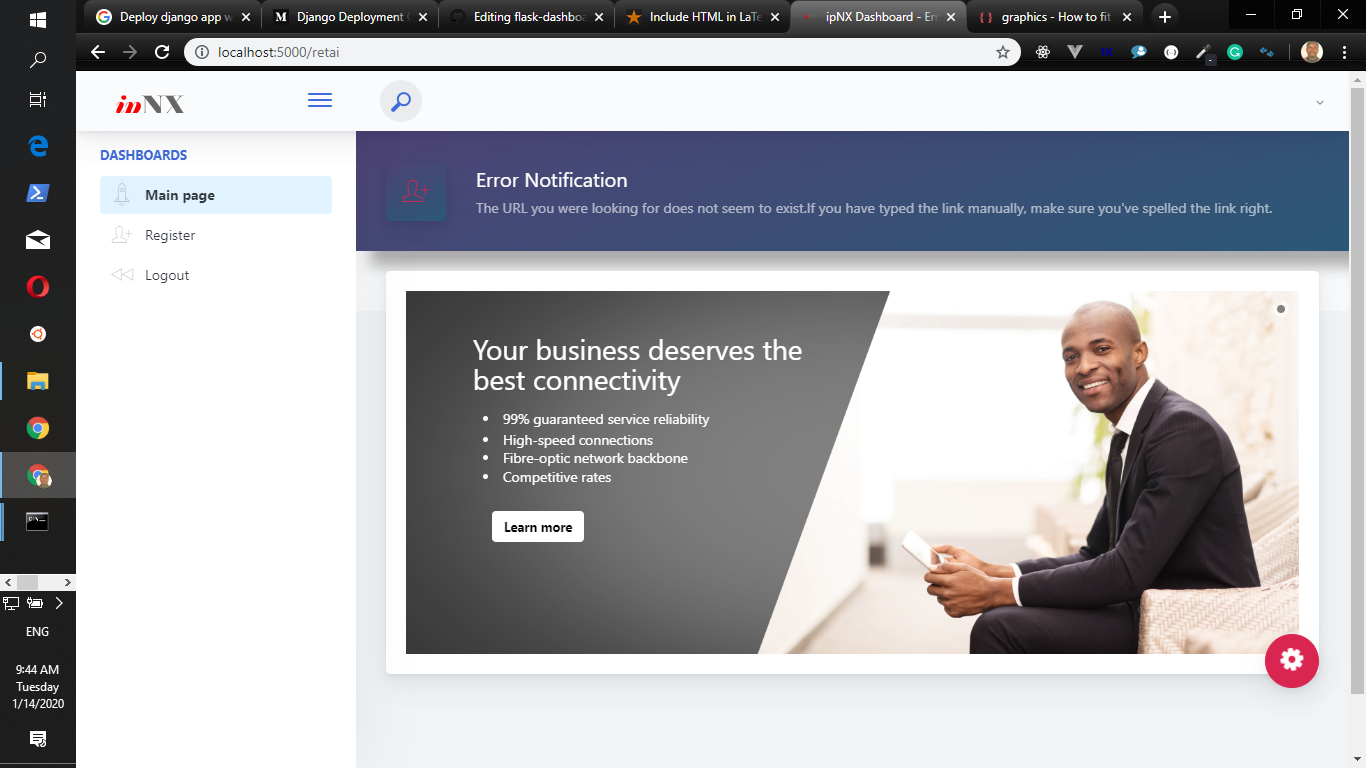
\includegraphics[width=\linewidth]{./duaerror}
		\caption{DUA dashboard Animated Error page}
	\end{subfigure}
		\caption{Re-designed DUA dashboard pages.}
	\end{figure}
\end{itemize}
\subsubsection{Django Blog}
\begin{itemize}
	\item \textbf{Project's description}: \textbf{Devc}, the name of the blog, is a complex web application inspired by \textbf{Frances Nnamadim}, a senior and regular colleague who worked as a Business Analyst and \ac{UI}/\ac{UX} designer in \textit{ip}NX's department of Business Intelligence and Data Analytics (BIDA). It was fully implemented in Django framework with PostgreSQL database at the back-end and a template initially designed by \href{https://www.styleshout.com/}{Styleshout}.\\
	
	\textbf{Devc} was built with three (3) other main applications embedded, each embedding other systems in turn:
	\subitem \textbf{Account management system}: This application provides interfaces for users registration and authentication. It allows direct authentication from popular social and technical websites such as Facebook, Twitter and Github among others as shown in Figure 3.9.
	\begin{figure}[!htbp]
		\centering
		\begin{subfigure}[b]{0.45\textwidth}
			\centering
			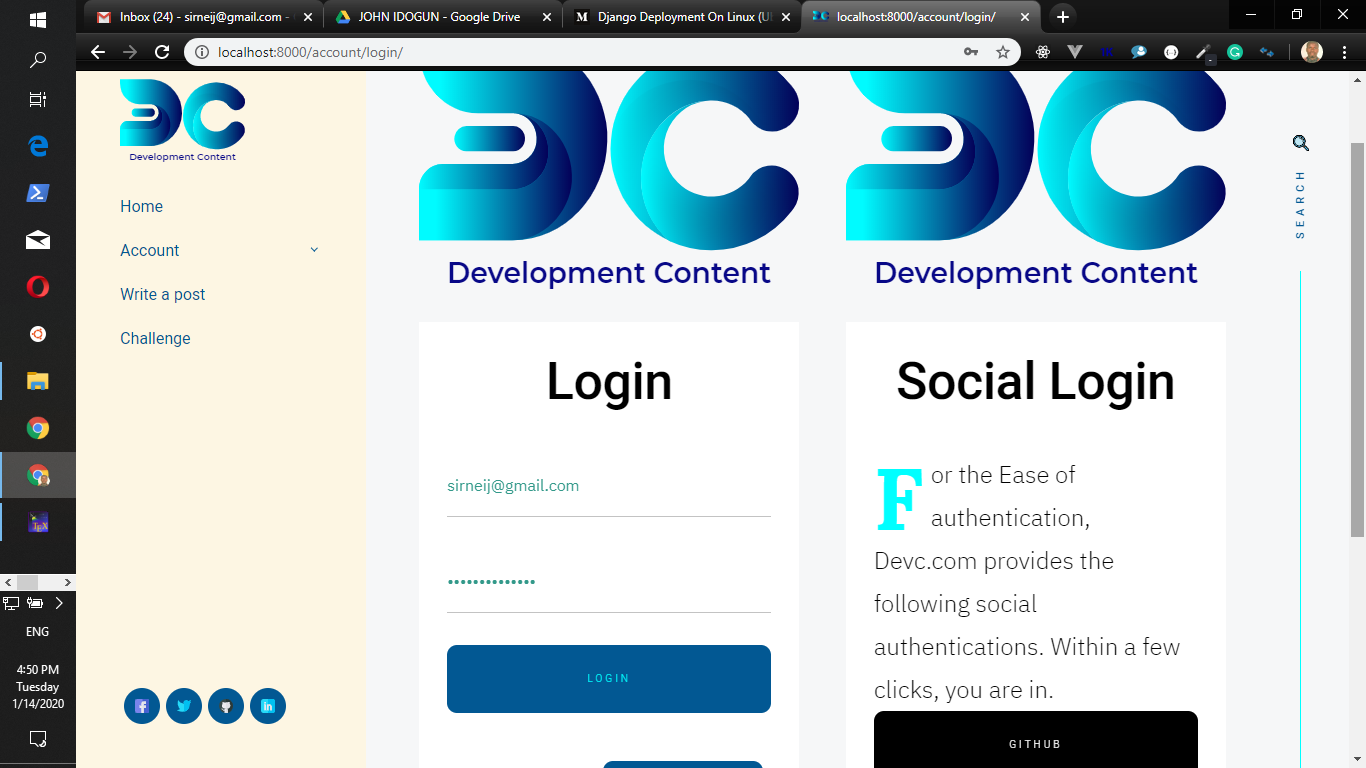
\includegraphics[width=\linewidth]{./devclogin}
			\caption{\textbf{devc} Login page with social authentication}
		\end{subfigure}
		\hfill
		\begin{subfigure}[b]{0.45\textwidth}
			\centering
			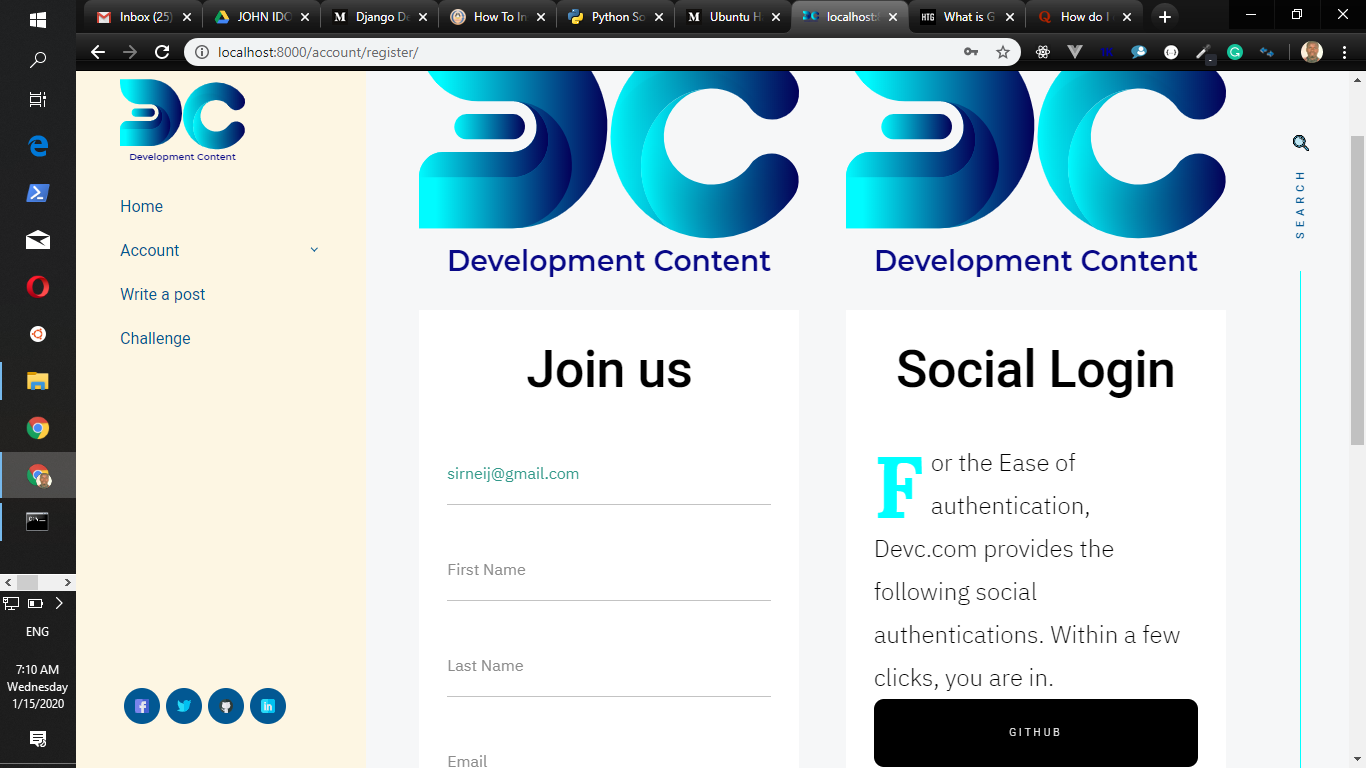
\includegraphics[width=\linewidth]{./devcsignup}
			\caption{\textbf{devc} Signup page with social authentication}
		\end{subfigure}
		\medskip
		\begin{subfigure}[b]{0.5\textwidth}
			\centering
			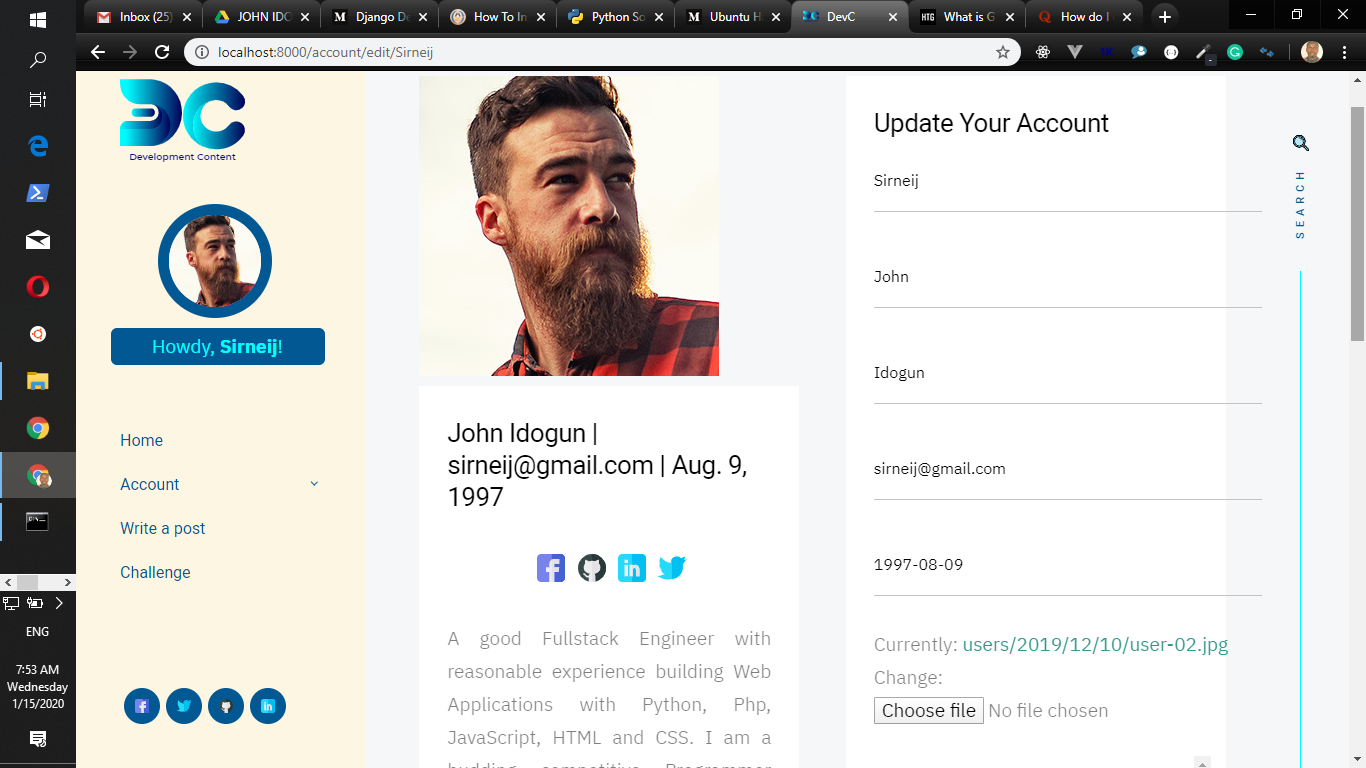
\includegraphics[width=\linewidth]{./devcaccount}
			\caption{\textbf{devc} Account update page}
		\end{subfigure}
		\caption{\textbf{devc} Account management system.}
	\end{figure}
	\subitem \textbf{Blogging system}: This is the heart of the overall system. It controls user's posts - their creation and  update, with a rich text editor and advanced text formatting system; and posts' deletion - profiles and portfolio with various mini-systems such as full-text search engine, tagging, related-posts recommendation, threaded commenting and slack-like chatting systems, embedded. Users' posts could also be liked and shared asynchronously. Some of these features are shown in Figure 3.10.
	\begin{figure}[!htbp]
		\centering
		\begin{subfigure}[b]{0.45\textwidth}
			\centering
			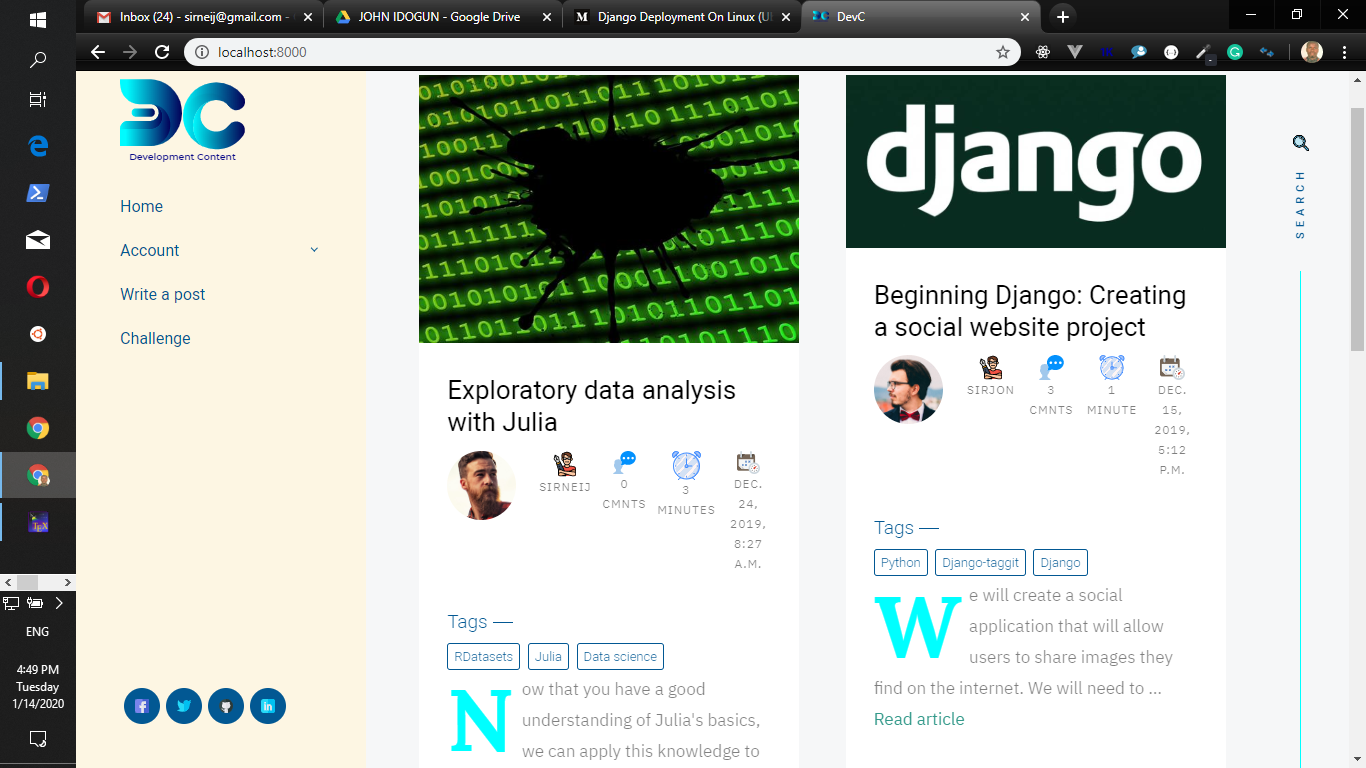
\includegraphics[width=\linewidth]{./devcmainwithout}
			\caption{\textbf{devc} main page without user authentication}
		\end{subfigure}
		\hfill
		\begin{subfigure}[b]{0.45\textwidth}
			\centering
			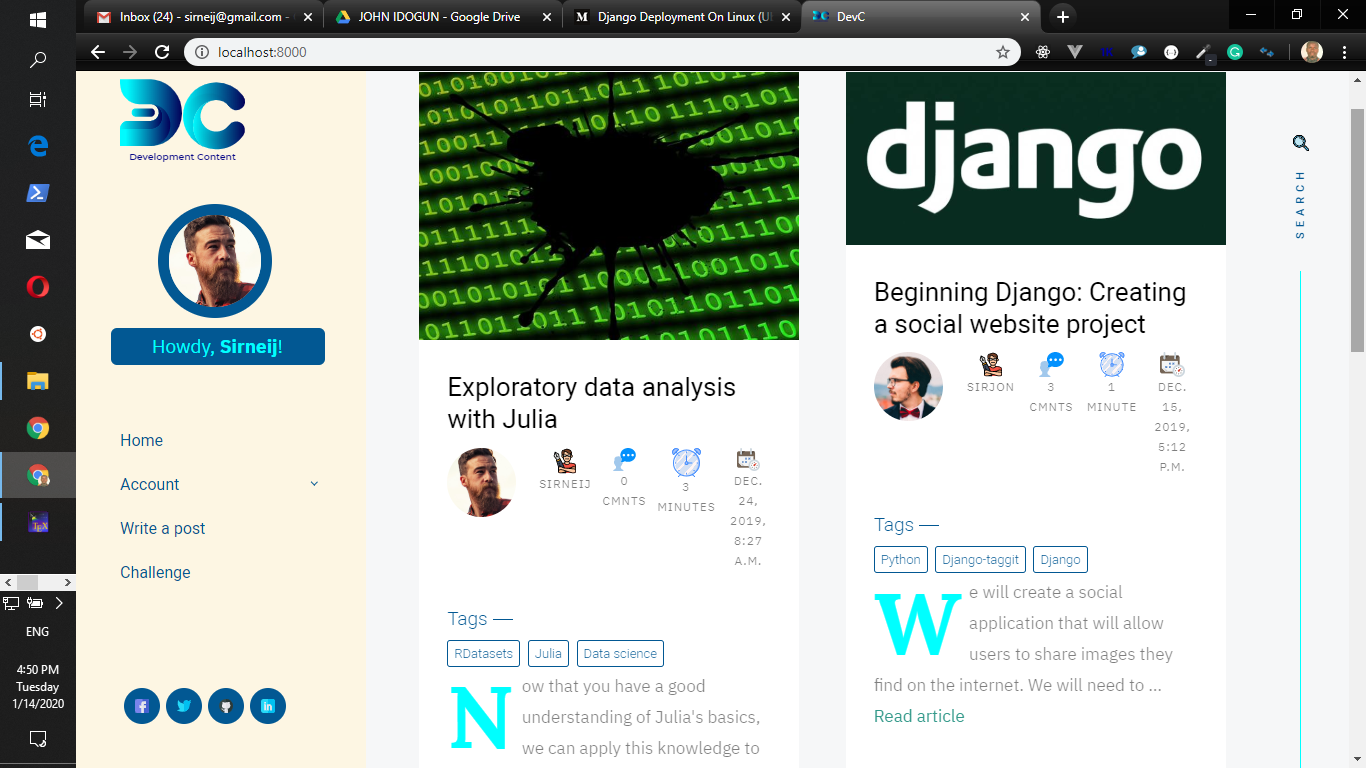
\includegraphics[width=\linewidth]{./devcmainwith}
			\caption{\textbf{devc} main page with user authentication, recent posts shown first.}
		\end{subfigure}
	\medskip
	\begin{subfigure}[b]{0.45\textwidth}
		\centering
		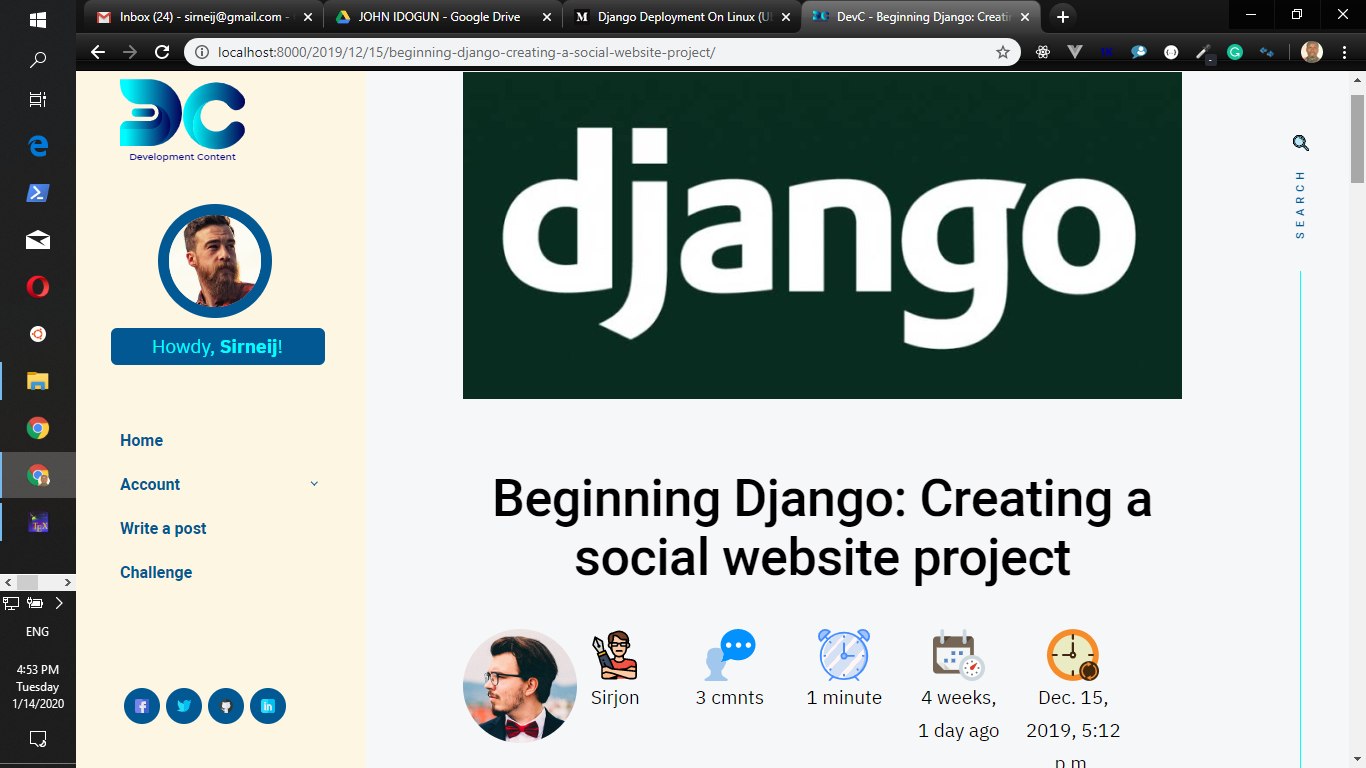
\includegraphics[width=\linewidth]{./devcpostdetail}
		\caption{\textbf{devc} Post detail page with user authentication}
	\end{subfigure}
	\hfill
	\begin{subfigure}[b]{0.45\textwidth}
		\centering
		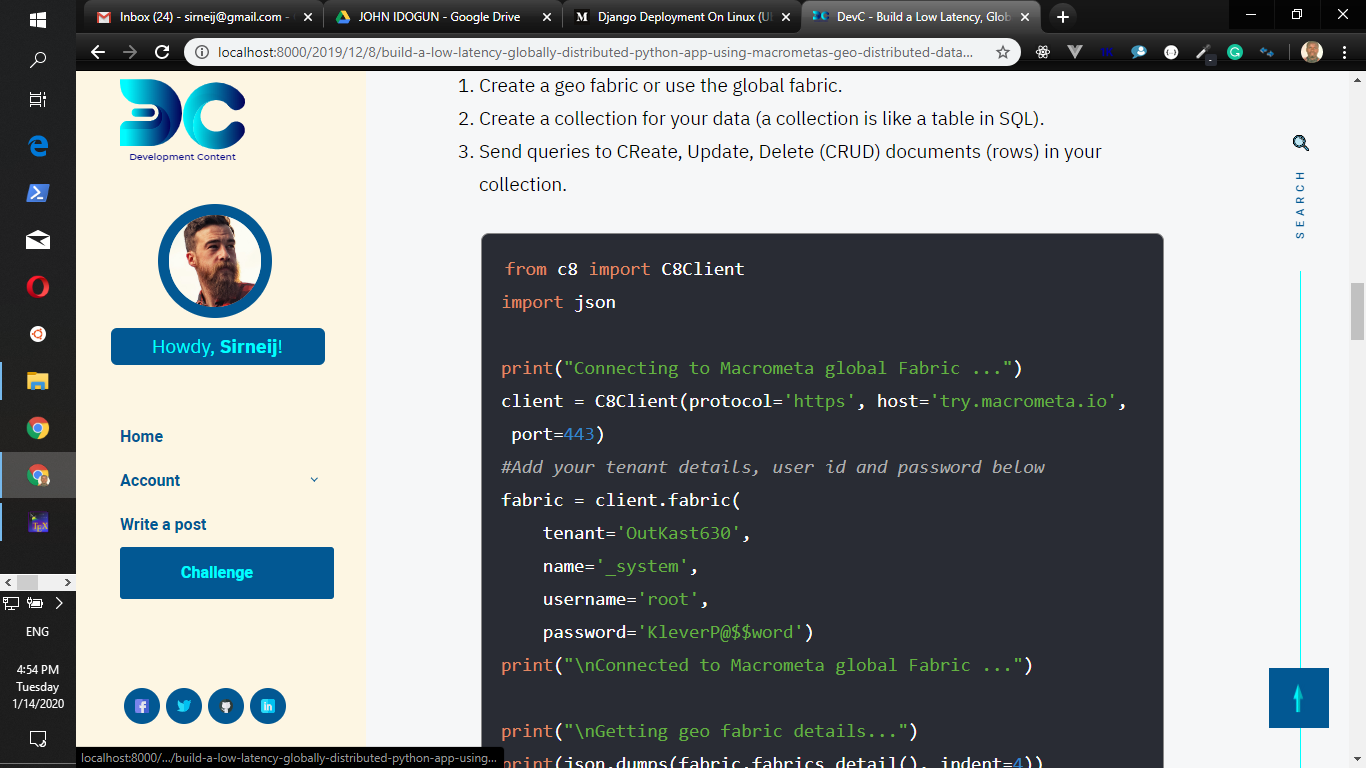
\includegraphics[width=\linewidth]{./devcpostdetailwith}
		\caption{\textbf{devc} syntax highlighting feature of the post detail page}
	\end{subfigure}
	\medskip
	\begin{subfigure}[b]{0.45\textwidth}
		\centering
		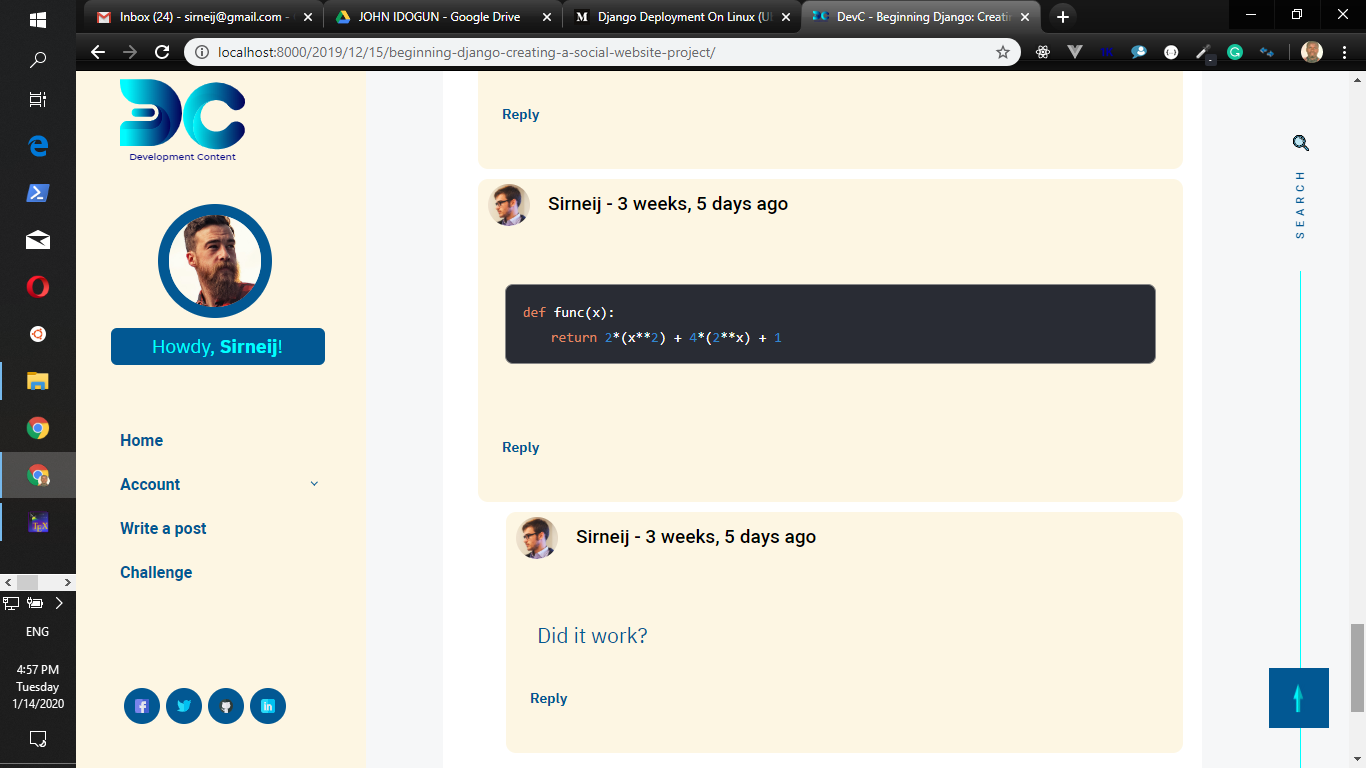
\includegraphics[width=\linewidth]{./devccomments}
		\caption{\textbf{devc} Threaded commenting section of the post detail page}
	\end{subfigure}
	\hfill
	\begin{subfigure}[b]{0.45\textwidth}
		\centering
		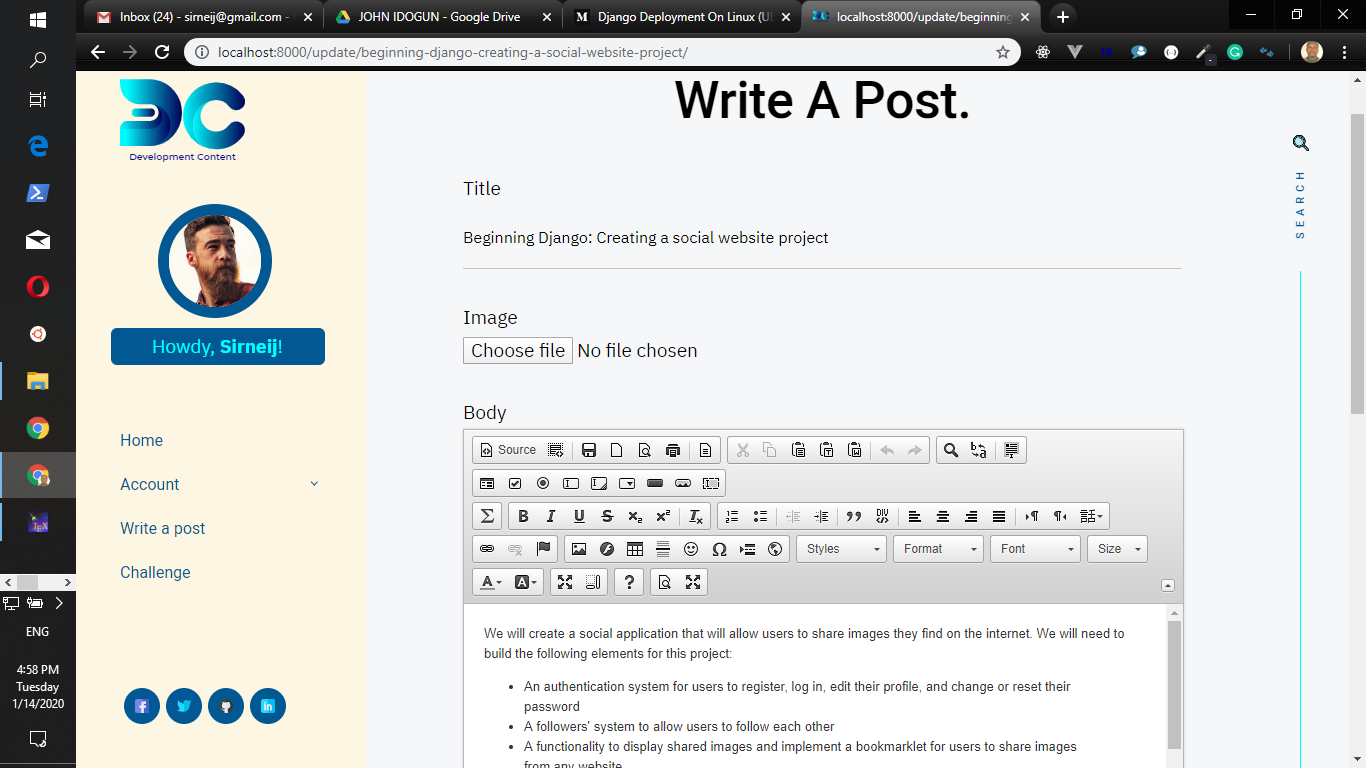
\includegraphics[width=\linewidth]{./devcpostupdate}
		\caption{\textbf{devc} post creation and update page with a Rich text editor}
	\end{subfigure}
		\caption{\textbf{devc} Blogging system.}
	\end{figure}
	\subitem \textbf{Portfolio system}: This serves as an extension of the account management system where authors of post(s) showcase their skills to their potential recruiters. It structures authors profiles, education, skills, projects and recommendations accordingly which can be downloaded in Portable Document Format (PDF). Figure 3.11 gives a quick tour of some of these features.
	\begin{figure}[!htbp]
		\centering
		\begin{subfigure}[b]{0.45\textwidth}
			\centering
			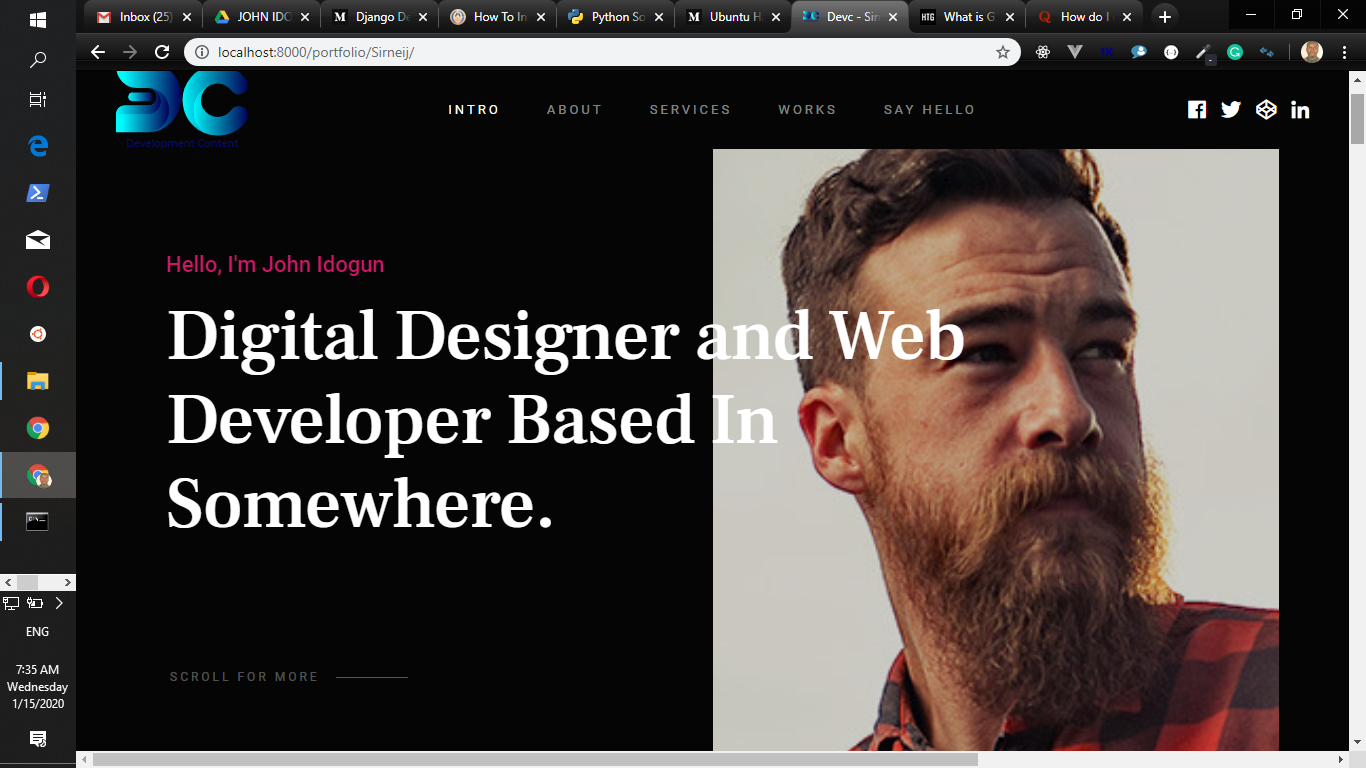
\includegraphics[width=\linewidth]{./devcportprofile}
			\caption{\textbf{devc} portfolio introduction section.}
		\end{subfigure}
		\hfill
		\begin{subfigure}[b]{0.45\textwidth}
			\centering
			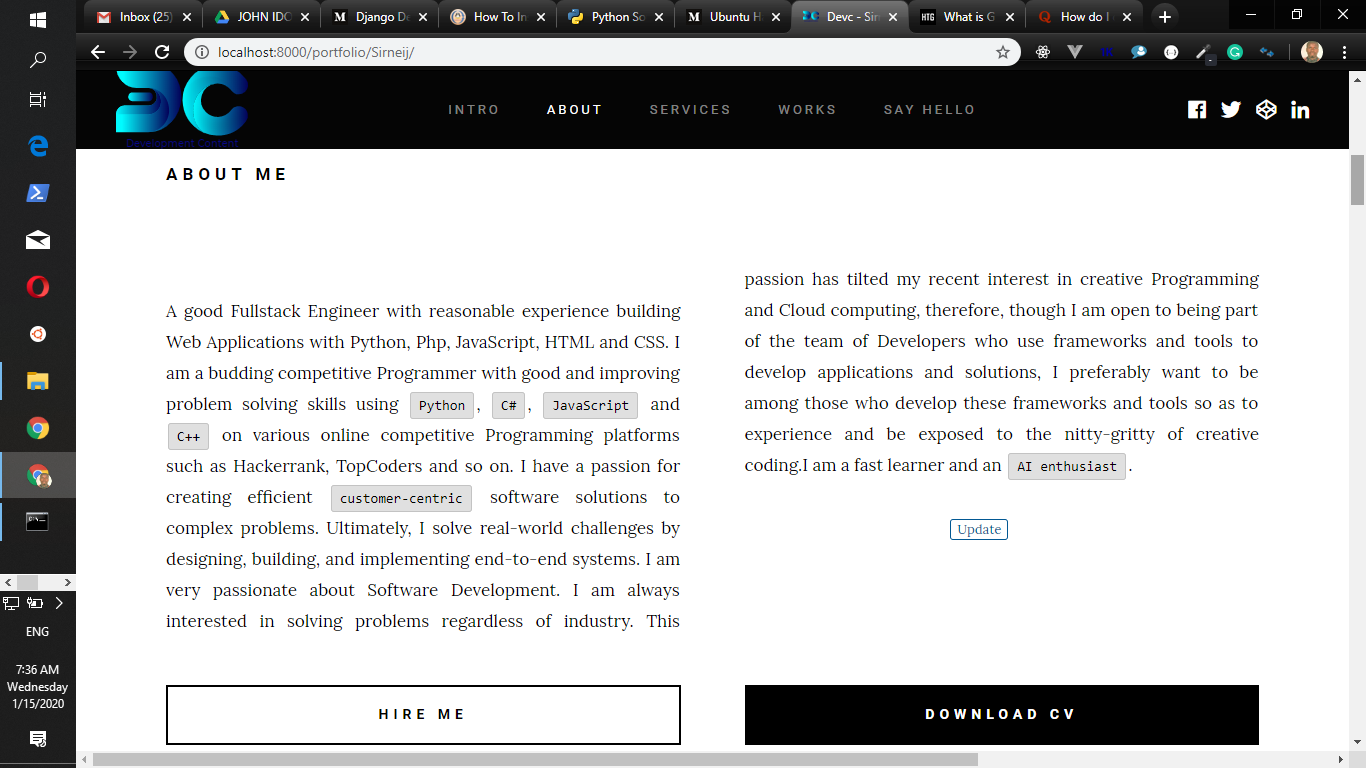
\includegraphics[width=\linewidth]{./devcportabout}
			\caption{\textbf{devc} portfolio about section.}
		\end{subfigure}
		\medskip
		\begin{subfigure}[b]{0.45\textwidth}
			\centering
			
\includegraphics[width=\linewidth]{./devcportwork}
			\caption{\textbf{devc} portfolio experience section}
		\end{subfigure}
		\hfill
		\begin{subfigure}[b]{0.45\textwidth}
			\centering
			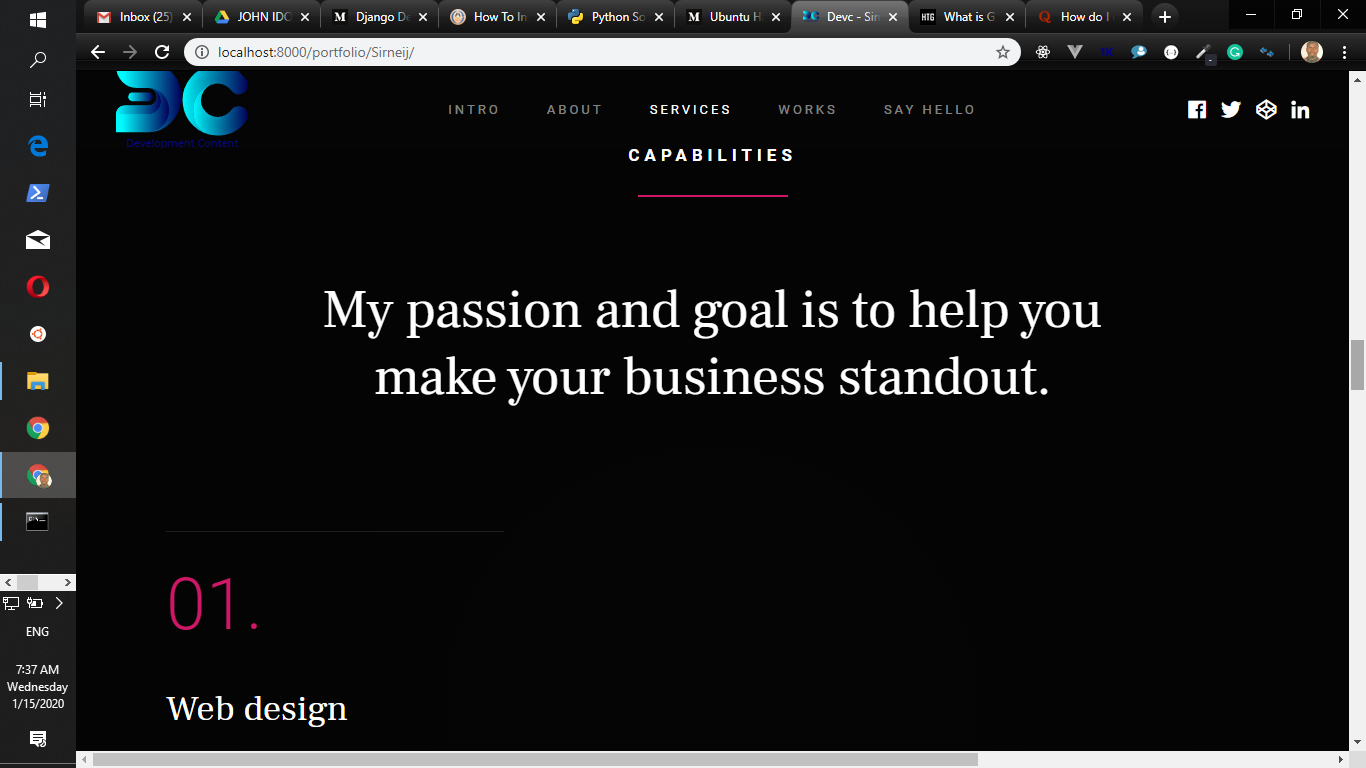
\includegraphics[width=\linewidth]{./devcportservices}
			\caption{\textbf{devc} portfolio service section}
		\end{subfigure}
		\medskip
		\begin{subfigure}[b]{0.45\textwidth}
			\centering
			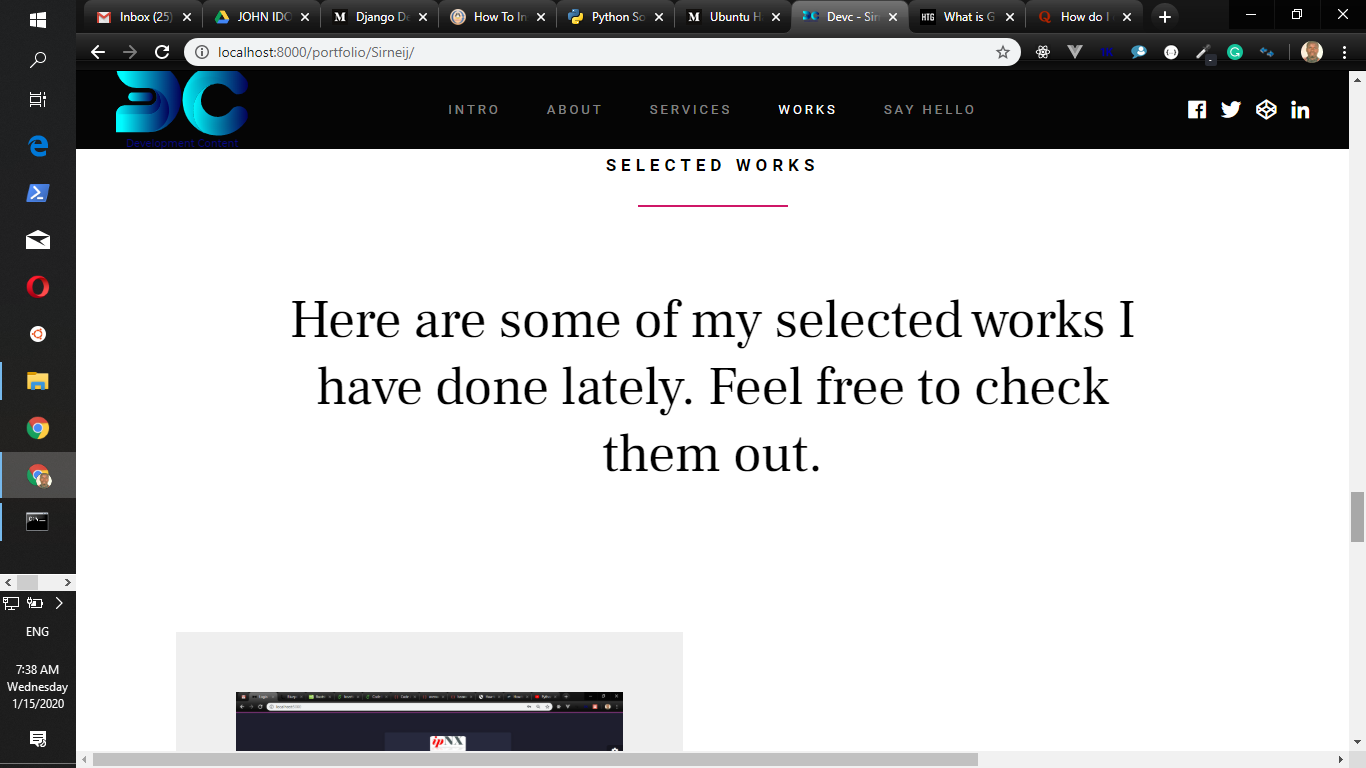
\includegraphics[width=\linewidth]{./devcportproject}
			\caption{\textbf{devc} portfolio project showcase section}
		\end{subfigure}
		\hfill
		\begin{subfigure}[b]{0.45\textwidth}
			\centering
			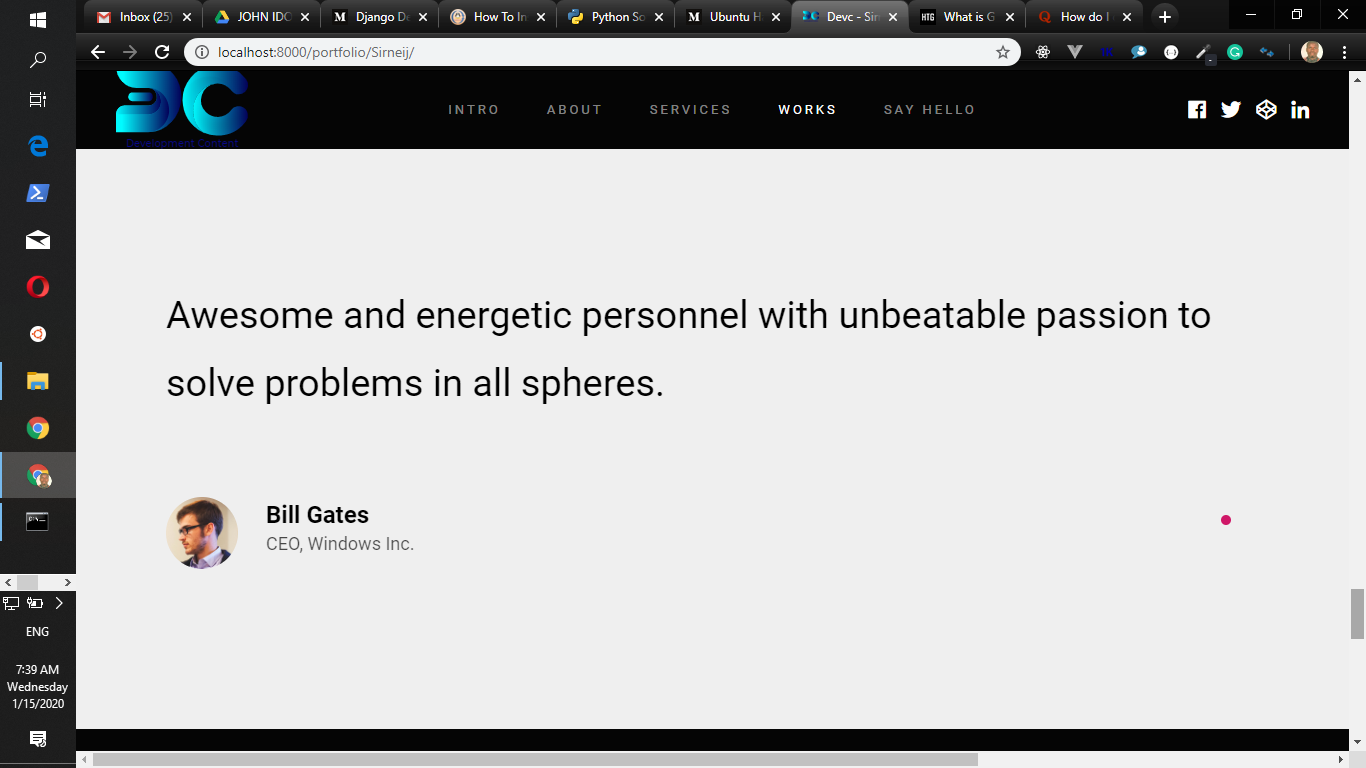
\includegraphics[width=\linewidth]{./devcportrecommend}
			\caption{\textbf{devc} portfolio recommendation section}
		\end{subfigure}
		\medskip
		\begin{subfigure}[b]{0.5\textwidth}
			\centering
			\includegraphics[width=\linewidth]{./devcportgetintouch}
			\caption{\textbf{devc} portfolio Get-in-touch section}
		\end{subfigure}
		\caption{\textbf{devc} Portfolio system.}
	\end{figure}
\end{itemize}
\section{Julia-based projects}
\subsection{Brief Introduction to Julia Programming Language}
Julia, a new programming language offering a unique combination of performance and productivity that promises to change scientific computing and programming in general, is an open-source language for high-performance technical computing and data science created by Jeff Bezanson, Stefan Karpinski, Viral B. Shah, and Alan Edelman, some of the best minds in mathematical and statistical computing, and first released in 2012.\\ 

It picks the best parts of existing programming languages, providing out-of-the-box features such as a powerful \ac{REPL}, an expressive syntax, Lisp-style metaprogramming capabilities, powerful numeric and scientific programming libraries, a built-in package manager, efficient Unicode support, and easily called C and Python functions, \citet{Salceanu:2018}.
\subsection{Web Crawler}
Web crawler is a program that implements web scraping, a technique for extracting data from web pages using software, and it
is a pivotal component of data harvesting.\\

The essence of this web scraping script was to harvest some from the \textbf{devc} blog for proper usage in a Wiki game, a project yet to be concluded. Code Snippet gives the source code of the web crawler.
\begin{code}
	\captionof{listing}{webcrawler.jl}
	\begin{minted}
[
breaklines,
frame=lines,
framesep=2mm,
baselinestretch=1,
fontsize=\footnotesize,
linenos
]
{Julia}
using HTTP, Gumbo
const PAGE_URL = "http://localhost:8000/"
const LINKS = String[]

function fetchPage(url)
	response = HTTP.get(url)
	# if response.status == 200 && parse(Int,
	Dict(response.headers)["Content-Length"]) > 0
	#     String(response.body)
	# else
	#     ""
	# end # if
	response.status == 200 && parse(Int,
	Dict(response.headers)["Content-Length"]) > 0 ?
	String(response.body) : ""
end # function

function extractlinks(elem)
	if isa(elem, HTMLElement) && tag(elem) == :a && in("href",
	collect(keys(attrs(elem))))
		url = getattr(elem, "href")
		#startswith(url, "/portfolio/") && push!(LINKS, url)
		startswith(url, "/2019/") && ! occursin(":", url) 
			&& push!(LINKS, url)
	end
	for child in children(elem)
		extractlinks(child)
	end
end # function


content = fetchPage(PAGE_URL)
if ! isempty(content)
	dom = Gumbo.parsehtml(content)
	extractlinks(dom.root)
end # if
display(unique(LINKS))
	
	\end{minted}
\end{code}
\section{Software Deployment}
Software Deployment involves packaging up software products and putting them in a production environment where they can be run since having them only on the local machine barricades access to them. A production environment is the canonical version of the locally housed application and its associated data.
\subsection{Python web application deployment}
Python web application deployments are comprised of many pieces that need to be individually configured. Figure 3.12 is a map that visually depicts how each deployment topic relates to each other.
\begin{figure}[!htbp]
	\centering
	\includegraphics[width=1\textwidth]{./deploy.png}
	\caption{Python web application deployment map, from \citet{Makai:2020}}
\end{figure}
\subsection{Deployement hosting option}
According to \citet{Makai:2020}, four options are available for deploying and hosting web applications, namely:
\begin{enumerate}
	\item "Bare metal" servers
	\item Virtualized servers
	\item Infrastructure-as-a-service
	\item Platform-as-a-service
\end{enumerate}
The first three options require the deployer to be provided with one or more servers having a Linux distribution wherein system packages, a web server, \ac{WSGI} server, database and the Python environment are then installed. There then the application can be pulled from source and installed in the environment.

This was the option through which the projects built were deployed and below is a comprehensive work-through for the applications deployment.
\subsection{Python applications deployment: General setup}
\begin{itemize}
	\item Having been provided with a remote private server based on Ubuntu 16.04 LTS with the ip address 10.50.0.20 and a password, the server was logged into using \ac{SSH}.
	\mint{bash}{~$ ssh jidogun@10.50.0.20}
	This required a password and was inputted appropriately.
	\item As it is one of the best practises to update a server when one logs in, the Linux distribution was updated.
	\mint{bash}{~$ sudo apt-get update}
	\item Python requires its Package manager, \mintinline{python}{pip}, to install its dependencies easily, therefore, it was installed alongside the proxy server used, \mintinline{nginx}{nginx} and \mintinline{nginx}{git}.
	\mint{bash}{~$ sudo apt-get install python-pip nginx git}
	\item As expected, \mintinline{nginx}{nginx} comes with a default configuration file which can be found in a \mintinline{nginx}{/etc/nginx/sites-enabled/}. This was removed to allow personalised configuration.
	\mint{bash}{~$ sudo rm /etc/nginx/sites-enabled/default}
	\item Having gotten rid of that default file, a personalised configuration file was created.
	\mint{bash}{~$ sudo touch /etc/nginx/sites-available/file_name}
	where \mintinline{bash}{file_name} is the desired name given to the file. It was called \mintinline{bash}{app_settings} in my case, so:
	\mint{bash}{~$ sudo touch /etc/nginx/sites-available/app_settings}
	\item Since the just created file needed to be active for its contents to be used by \mintinline{nginx}{nginx}, a symbolic file, pointing to the \mintinline{nginx}{app_settings} file created above, was made in \mintinline{nginx}{/etc/nginx/sites-enabled/app_settings}.
	\begin{minted}
		[breaklines]
		{bash}
~$ sudo ln -s /etc/nginx/sites-available/app_settings /etc/nginx/sites-enabled/app_settings
	\end{minted}
	\item The symbolic file made above was edited using \mintinline{nginx}{nano} editor, to cater for all the applications to be deployed using different port numbers:
	\mint{bash}{~$ sudo nano /etc/nginx/sites-enabled/app_settings}
	\begin{code}
		\captionof{listing}{/etc/nginx/sites-enabled/app\_settings}
		\begin{minted}
[
breaklines,
frame=lines,
framesep=2mm,
baselinestretch=1,
fontsize=\footnotesize,
linenos
]
{nginx}
server {
	listen 8004;
	location / {
		include proxy_params;
		proxy_pass http://127.0.0.1:8000;
	}
}
server {
	listen 8001;
	location / {
		include proxy_params;
		proxy_pass http://127.0.0.1:8008;
	}
}
server {
	listen 8002;
	location / {
		include proxy_params;
		proxy_pass http://127.0.0.1:8888;
	}
}
server {
	listen 8003;
	location / {
		include proxy_params;
		proxy_pass http://127.0.0.1:8999;
	}
}
		\end{minted}
	\end{code}
	Four server instances were created since four applications were deployed. The first instance pointed to Django blog, since the default port for django applications is 8000. The rest instances were used for the three dashboards written in flask.
	\item Next, \mintinline{nginx}{nginx} was restarted.
	\mint{bash}{~$ sudo systemctl restart nginx}
\end{itemize}
With the above configurations, everything regarding \mintinline{nginx}{nginx} was pretty much done with. The next inline was to deal with framework-specific configurations.
\subsection{Framework-specifics}
Before getting started with the framework-specific configurations, it was deemed necessary to organize the applications based on frameworks. Thus, different folders were created.
\mint{bash}{~$ mkdir flask_app django_app}
Obviously, all flask-based applications would take \mintinline{bash}{flask_app} directory as their habitat while \mintinline{bash}{django_app} would house django-based applications. The applications were cloned from their respective github repositories into either of these folders as appropriate.
\subsubsection{Flask}
First off, all flask-based applications were cloned into \mintinline{bash}{flask_app} directory.
\begin{minted}
[breaklines]
{bash}
~/flask_app$ git clone https://github.com/Sirneij/CPE-dash.git
~/flask_app$ git clone https://github.com/Sirneij/CEA-dash.git
~/flask_app$ git clone https://github.com/Sirneij/DUA-dash.git
\end{minted}
Thence, the undermentioned operations were performed on each of them, using \mintinline{bash}{CPE-dash} as an instance for clarification.
	\begin{itemize}
		\item First off, directory was changed to \mintinline{bash}{CPE-dash}
		\mint{bash}{~/flask_app$ cd CPE-dash}
		\item A virtual environment for the application must be created to avoid Python version conflict issues. But First, \mintinline{nginx}{virtualenv} was installed.
		\mint{bash}{~/flask_app/CPE-dash$ sudo pip install virtualenv}
		\item Next, a virtual environment was created for it, specifying the python version to be used(since all the applications required at least python3.6 to function optimally, it was selected as the python version to be used).
		\mint{bash}{~/flask_app/CPE-dash$ virtualenv -p /usr/bin/python3.6 cpe #Environment name.}
		\item Having created the virtual environment, it was activated.
		\mint{bash}{~/flask_app/CPE-dash$ source cpe/bin/activate}
		\item That done, the application's dependencies, stored in \mintinline{nginx}{requirements.txt} file, and the real Python server, \mintinline{nginx}{gunicorn} were installed.
		\mint{bash}{(cpe):~/flask_app/CPE-dash$ sudo pip install -r requirements.txt gunicorn}
		\item Penultimately, the applications \mintinline{python}{run.py} was edited to reflect the host and port configured in \mintinline{nginx}{/etc/nginx/sites-enabled/app_settings}, leaving the first server instance for django.
		\mint{bash}{(cpe):~/flask_app/CPE-dash$ sudo nano run.py}
		\begin{code}
			\captionof{listing}{(cpe):~/flask\_app/CPE-dashapp/run.py}
			\begin{minted}
[
breaklines,
frame=lines,
framesep=2mm,
baselinestretch=1,
fontsize=\footnotesize,
linenos
]
{python}
from app import create_app
from app import db
app = create_app()
db.create_all(app=create_app())
if __name__ == '__main__':
	app.run(host="0.0.0.0", port=8008, debug=False)	
			\end{minted}
		\end{code}
		\item Finally, \mintinline{nginx}{gunicorn} was called and subsequently served with the main app's file name(without .py extension), in this case, \mintinline{nginx}{run}
		\mint{bash}{(cpe):~/flask_app/CPE-dash$ gunicorn run:app -b 127.0.0.1:8008 &}
		\textbf{That was it! Application was successfully deployed! This procedure was repeated to deploy the other two flask apps.}
	\end{itemize}
 To confirm, a browser was initiated and the ip address of the server provided as well as the port the app was listening to, say \textbf{10.50.0.20:8001} (for CPE-dash), was inputted as \ac{URL} or web address and it returned a full version of the initial app.
 
 \subsubsection{Django}
 The steps observed in deploying flask-based and Django-based applications are almost the same aside some of the dependencies that django requires. Also, the developed blog used PostgreSQL database instead of SQLite which must be installed and configured specially for the application to execute smoothly. 

 Getting started, PostgreSQl and its dependencies were installed.
 \begin{minted}
 [breaklines]
 {bash}
 ~$ sudo apt-get install python3-dev libpq-dev postgresql postgresql-contrib
 \end{minted} 
\textbf{CAVEAT}: It's extremely important to successfully install \mintinline{python}{python3-dev} and \mintinline{python}{libpq-dev} as they are the build prerequisites which must be met in order to install \mintinline{python}{Psycopg}, a PostgreSQL adapter for the Python programming language, from a source distribution package. \mintinline{python}{Python3-dev(or python-dev)} provides the header files and its absence results in \textit{error: Python.h: No such file or directory} when installing psycopg or psycopg2 as the case may be. \mintinline{python}{libpq} header files are provided in the \mintinline{python}{libpq-dev} package. \textit{error: libpq-fe.h: No such file or directory} is thrown if the package is not installed.

If the above command did not install these dependencies properly, use:
\begin{minted}
[breaklines]
{bash}
~$ sudo apt-get install python3.6-dev libpq-dev postgresql postgresql-contrib #specify the python version used
\end{minted}
Next, a database user and database for the Django app were created:
\begin{minted}
[breaklines]
{postgres}
~$ sudo su - postgres #changes to postgres environment
postgres@10.50.0.20:~$ createuser --interactive -P
Enter name of role to add: devc #adds devc
Enter password for new role: 
Enter it again: 
Shall the new role be a superuser? (y/n) n
Shall the new role be allowed to create databases? (y/n) n
Shall the new role be allowed to create more new roles? (y/n) n
\end{minted}
The commands about created a database user \mintinline{postgres}{devc} and assigned roles to it.
\begin{minted}
[breaklines]
{postgres}
postgres@10.50.0.20:~$ createdb --owner devc django_app_db #creates django_app_db using devc user
\end{minted}
Having added a user and a database, logging out of the postgres environment was done.
\mint{postgres}{postgres@10.50.0.20:~$ logout}
Directory was changed into \mintinline{bash}{django_app} and the app was cloned from github. Thence, directory was changed into the cloned app directory.
\begin{minted}
[breaklines]
{bash}
~$ cd django_app
~/django_app$ git clone https://github.com/Sirneij/devcAll.git
~/django_app$ cd devcAll
\end{minted}
The \mintinline{python}{settings.py} file of the app located in \mintinline{bash}{/devc/devc} directory was modified to configure the database settings created above. The host was also set.
\begin{minted}
[breaklines]
{bash}
~/django_app/devcAll$ nano /devc/devc/settings.py
\end{minted}

\begin{code}
	\captionof{listing}{/devc/devc/settings.py}
	\begin{minted}
[
breaklines,
frame=lines,
framesep=2mm,
baselinestretch=1,
fontsize=\footnotesize,
linenos
]
{python}
...	
DATABASES = {
	'default': {
		'ENGINE': 'django.db.backends.postgresql_psycopg2',                                                                                 'NAME': 'django_app_db',
		'USER': 'devc',
		'PASSWORD':'',#input your password
		'HOST': 'localhost',
		'PORT': '',
	}
}

ALLOWED_HOSTS = ['*']#you could have input your ip address or domain name instead. '*' is for simplicity.
...
	\end{minted}
\end{code}

To effect the changes made, migrations were made, super user was created and static files were collected.

\begin{minted}
[breaklines]
{bash}
~/django_app/devcAll$ cd devc #changes directory to devc where manage.py is located
~/django_app/devcAll/devc$ python manage.py migrate  #Syncs the database.
~/django_app/devcAll/devc$ python manage.py collectstatic #collects the static files
(devcenv):~/django_app/devcAll$ python manage.py createsuperuser #creates the super user
Username(or 'jidogun' if not specified):
Email:
Password:
Password again:
\end{minted}

Django and PostgreSQl specifics concluded. Virtual environment was created and activated as demonstrated and specified under Flask app deployment above and requirements as well as gunicorn were installed and instantiated!
\begin{minted}
[breaklines]
{bash}
~/django_app/devcAll$ virtualenv -p /usr/bin/python3.6 devcenv #Creates devcenv virtual environment using python3.6 as interpreter.
~/django_app/devcAll$ source devcenv/bin/activate #activates virtual environment
(devcenv):~/django_app/devcAll$ sudo pip install -r requirements.txt gunicorn #installs dependencies and gunicorn
(devcenv):~/django_app/devcAll/devc$ gunicorn devc.wsgi -b 0.0.0.0:8000 & #serves gunicorn the app persistently.
\end{minted}

The applications could now be accessed online...

If error of the below form erupted:
\begin{minted}
[breaklines,
fontsize=\footnotesize
]
{bash}
[2020-01-20 15:08:02 +0000] [19640] [INFO] Starting gunicorn 19.4.5
[2020-01-20 15:08:02 +0000] [19640] [ERROR] Connection in use: ('0.0.0.0', 8000)
[2020-01-20 15:08:02 +0000] [19640] [ERROR] Retrying in 1 second.
[2017-01-20 15:08:03 +0000] [19640] [ERROR] Connection in use: ('0.0.0.0', 8000)
[2020-01-20 15:08:03 +0000] [19640] [ERROR] Retrying in 1 second.
[2020-01-20 15:08:04 +0000] [19640] [ERROR] Connection in use: ('0.0.0.0', 8000)
[2020-01-20 15:08:04 +0000] [19640] [ERROR] Retrying in 1 second.
[2020-01-20 15:08:05 +0000] [19640] [ERROR] Connection in use: ('0.0.0.0', 8000)
\end{minted}
Below commands would get them solved:
\begin{minted}
[breaklines,
fontsize=\footnotesize
]
{bash}
$ sudo netstat -nlp | grep :80 #finds the process using port 80
$ sudo fuser -k 8000/tcp #kills the process

#Reserve gunicorn with the application

(devcenv):~/django_app/devcAll/devc$ gunicorn devc.wsgi -b 0.0.0.0:8000 & #serves gunicorn the app persistently.
\end{minted}
\chapter{Conclusion and Recommendation}
\section{Conclusion}
During this internship, I had the chance to work on many aspects of Software Engineering ranging from the Planning and Requirement Analysis of software products to their actual development and eventual Deployment. I developed new technical knowledge and soft skills while improving or enhancing previous ones in the course of implementing the robust projects undertaken.
\begin{itemize}
	\item I gained new knowledge in the area of Working with PostgreSQL - for full-text search capabilities - and SQLite Databases, regarding the various issues involved and mechanisms in these systems.
	\item I brushed up my knowledge of Python and JavaScript, as they were required to implement the projects.
	\item It was a challenging but awesome experience deploying applications to a Linux server from the ground up. Countless times of breaking and fixing server dependencies were worth the stress after all as the process exposed nifty things about systems administration.
	\item The importance and huge impact portability and scalability have on decisions about hardware, technologies/tools to be used, system architecture, algorithms, and so on were duly learnt and observed.
	\item Extensive exposure to Git, as a version control system, for safe storage of codes and projects.
	\item Significant knowledge of using asynchronous programming for some background tasks to provide better user experience was well learnt.
	\item Hands-on experience engaging in cross-platform troubleshooting of software products.
	\item Total exposure to the Linux operating system, especially Ubuntu 14.04 LTS and 16.04 LTS, for software deployment using Apache2, nginx and gunicorn. 
\end{itemize}
Some theoretical knowledge gained in school proved helpful and useful such as CPE407(Software Development Techniques), a useful ingredient in following along with the software development processes at \textit{ip}NX Nigeria Limited, and CPE202(Programming in C Language) as well as CPE302(Object Oriented Programming using C\#), for laying a good foundation in programming to pick up other languages effortlessly.
\section{Recommendation}
There is no gainsaying the fact that the idea of Industrial Training is laudable and its role in equipping students with relevant and soft skills cannot be overemphasized. Out of the various things learned and experiences gained, the undermentioned are worth taking into consideration:
\begin{enumerate}
	\item \textbf{Adoption and Enforcement of Project Based Learning (PBL)}: Project Based Learning (PBL) is a pedagogy in which students learn by actively engaging in real-world and personally meaningful projects. In this method, students work on a project over an extended period of time – from a week up to a semester – that engages them in solving a real-world problem or answering a complex question.
	
	As a result, students develop deep content knowledge as well as critical thinking, collaboration, creativity, and communication skills. Project Based Learning unleashes a contagious, creative energy among students and teachers. Using and enforcing this method, with proper and decent design, will help narrow the wide gap between University Education and Industry required knowledge.
	\item \textbf{Incorporation of a full course on Algorithms and Data structures}: Data structure and associated algorithms are an important part of any computer science or engineering curriculum as they expose students to critical and advanced thinking skills which will ultimately ameliorate problem-solving prowess. It is highly important that students are aware of them because most Interview questions are based on their application.
	\item \textbf{Use of innovative approaches to teaching and
		learning}: The use of innovative approaches to teaching and
	learning is very essential such as the use of teaching aids, ensuring the availability of teaching materials online before and after lectures among others.
	\item The Federal Government should make it an obligation for all firms to absorb students on Industrial training and ensure that such students are well-trained. This stretches out of how daunting and herculean it is to secure a placement by most students.
\end{enumerate}


\bibliographystyle{apalike}
\bibliography{fydp}
\addcontentsline{toc}{chapter}{References}

\clearpage
%\appendix 

%\phantomsection

%\addcontentsline{toc}{chapter}{Appendices}
%\chapter{Amino Acids\label{appAmino}}
%\begin{figure}[h]
%\begin{center}
%\includegraphics[width=1\textwidth]{./images/background/aminoacids}
%\end{center}
%\caption{Twenty different amino acids, their structures and chemical properties.\index{Amino Acid!chemical properties}\cite{Lehninger2012}.}
%\end{figure}
%\clearpage
%\thispagestyle{empty}
%\mbox{}

%\clearpage
%\phantomsection
%\addcontentsline{toc}{chapter}{Index}
%\printindex

\end{document}
